\documentclass[
  normalmargins,
  11pt,
  openany,
  onehalfspacing,
]{ut-thesis}

% packages
\usepackage{etoolbox}
\usepackage{aasmacros}
\usepackage[round]{natbib}
\bibliographystyle{my_abbrvnat}

\usepackage[french,english]{babel}
\usepackage[utf8]{inputenc}
\usepackage[T1]{fontenc}

\newrobustcmd*{\andname}{et}
  \addto \extrasenglish {\renewrobustcmd*{\andname}{and}}
  \addto \extrasfrench  {\renewrobustcmd*{\andname}{et}}

\newrobustcmd*{\liaisonname}{et}
  \addto \extrasenglish {\renewrobustcmd*{\liaisonname}{and}}
  \addto \extrasfrench  {\renewrobustcmd*{\liaisonname}{et}}


\usepackage[autostyle]{csquotes} 
\usepackage{threeparttable}
\usepackage{epigraph}
\setlength{\epigraphwidth}{0.6\textwidth}
\setlength{\epigraphrule}{0pt}


\usepackage[colorlinks,
    linkcolor={black},
    citecolor={blue},
    urlcolor={black}]{hyperref} % for links
\usepackage{graphicx} % for embedding graphics
%\usepackage{booktabs} % for pretty tables
\usepackage{caption}
\usepackage{subcaption}
\usepackage[nottoc]{tocbibind} % adds lot and lof to toc
\usepackage{pdfpages}
\usepackage{float}
\usepackage{amsmath, bm, bbm}
\usepackage{amssymb}
\usepackage{mathtools}
\usepackage{physics}
\usepackage{cancel}
\usepackage{tikz}
\usetikzlibrary{arrows.meta}
\usepackage{enumitem}
\usepackage{lipsum}
\newcommand{\subscript}[2]{$#1 _ #2$}

\newcommand{\KL}{\mathrel{\Vert}}
\DeclareRobustCommand{\bbone}{\text{\usefont{U}{bbold}{m}{n}1}}
\DeclareMathOperator{\EX}{\mathbb{E}}% expected value

\def\frenchlistfigurename{Liste des figures}
\def\frenchlisttablename{Liste des tableaux}

\usepackage[nogroupskip,nonumberlist,acronym,toc,sort=def]{glossaries} 
\newglossary[slg]{symbolslist}{syi}{syg}{Symboles}
%\newglossary[slg]{acronyms}{syi}{syg}{Abbréviations}

\usepackage{glossary_entry}
\makeglossaries 

% author data
\author{Alexandre Adam}
\university{Université de Montréal}
\sujet{physique}
%\president{Yashar Hezaveh}
%\directeur{Laurence Perreault-Levasseur}
%\membrejury{René Doyon}
\faculty{Faculté des arts et des sciences}
\title{Reconstruction libre de lentilles gravitationnelles de type galaxie-galaxie avec les machines à inférence récurentielle}
%\title{La reconstruction d'image dans le contexte des problèmes inverses mal posées et non-linéaires avec les machines à inférence récurentielles}
\degree{Maître ès sciences (M.Sc.)}
\department{Département de physique}
\gradyear{2022}

\allowdisplaybreaks
\begin{document}
% Add items to glossary without displaying them
  \selectlanguage{french}
  \frontmatter
    \maketitle
    \maketitletwo
        \selectlanguage{french}
    \begin{resume}
	Les lentilles gravitationnelles de type galaxie-galaxie se produisent lorsque la lumière d'une galaxie 
	en arrière-plan est déviée par le champ gravitationnel d'une galaxie en avant-plan, formant 
	des images multiples ou même des anneaux d'Einstein selon le point de vue d'un observateur sur Terre. 
	Ces phénomènes permettent non seulement 
	d'étudier les galaxies lointaines, magnifiées par la galaxie-lentille, mais aussi de comprendre la distribution 
	de masse de la galaxie-lentille et de son environnement, une opportunité unique pour 
	sonder la matière noire contenue dans ces galaxies. 
	Or, les méthodes traditionnelles pour analyser ces systèmes requièrent une quantité 
	significative de temps ordinateur (de quelques heures à quelques jours), sans compter le temps des 
	experts pour faire converger les analyses MCMC requises pour obtenir les paramètres d'intérêts. 
	Ce problème est significatif, considérant qu'il est projeté que  
	les grands relevés du ciel comme ceux qui seront menés aux observatoires Rubin et Euclid découvrirons plusieurs 
	centaines de milliers de lentilles gravitationnelles.  
	De plus, le Télescope géant européen (ELT), faisant usage de la technologie d'optique adaptative, 
	et le télescope spatial James Webb, vont nous offrir une vue sans précédent de ces systèmes, avec un 
	pouvoir de résolution qui rendra possible certaines analyses comme la recherche de halo de matière noire froide, 
	longtemps prédite par le modèle cosmologique standard $\Lambda$CDM. Les approximations traditionnelles faites pour 
	simplifier la reconstruction des lentilles gravitationnelles ne seront plus valides dans ce régime.

	Dans ce mémoire, je présente un travail qui s'attaque à ces deux problèmes. Je présente une 
	méthode d'optimisation basée sur les machines à inférence récurentielle pour reconstruire 
	deux images, soit celle d'une galaxie en arrière-plan et une image pour la distribution de masse 
	de la galaxie en avant-plan. La représentation paramétrique choisie a le potentiel de reconstruire 
	une classe très large de lentilles gravitationnelles, incluant des halos et sous-halos de matière noire, 
	ce qu'on démontre dans ce travail en utilisant des profiles de densité réalistes provenant de 
	la simulation cosmologique hydrodynamique IllustrisTNG. 
	Nos reconstructions atteignent un niveau de réalisme jamais atteint auparavant 
        et s'exécutent sur une fraction du temps requis pour exécuter une analyse traditionnelle, soit un pas 
	significatif vers une méthode pouvant adresser le défi d'analyser autant de systèmes complexes et variés en 
	un temps à l'échelle humaine.

    \end{resume}

	\selectlanguage{english}
    \begin{abstract}
	Galaxy-Galaxy gravitational lenses is a phenomenon that happens when the light, coming from a background 
	galaxy, is bent by the gravitational field of a foreground galaxy, producing multiple images or even 
	Einstein ring images of the background source from the point of view of an observer on Earth.
	These phenomena allow us to study in detail the morphology of the background galaxy, magnified 
	by the lens, but also study the mass density distribution of the lens and its environment, thus offering a 
	unique probe of dark matter in lensing galaxies.
	But traditional methods studying these systems often need significant compute time (from hours to days), 
	and this is without taking into account the time spent by experts 
	to make the MCMC chains required to obtain parameters 
	of interest converge. This problem is significant, considering that 
	large surveys from observatories like Rubin and Euclid are projected to discover hundreds of thousands of 
	gravitational lenses. Moreover, the Extremely Large Telescope (ELT), using adaptive optics, and the 
	James Webb Space Telescope will offer an unprecedented glimpse of these systems, with a resolving power 
	predicted to enable searches for cold dark matter subhalos, long predicted by the standard cosmological model
	$\Lambda$CDM. Approximations used in traditional methods to make analysis tractable will no longer be valid 
	in that regime.

	In this thesis, I present a method that aims to address these two issues. The method, 
	based on Recurrent Inference Machines (RIM), reconstructs two pixelated maps, one for the 
	background source and another for the mass density map of the foreground lensing galaxy. 
	This free-form parametric representation has the potential to reconstruct a large class 
	of gravitational lenses, including those with dark matter halos and subhalos, which 
	we demonstrate using realistic mass density profiles from the cosmological 
	hydrodynamic simulation IllustrisTNG.
	Our method can achieve an unmatched level of realism in a fraction of the time required by traditional methods, 
	which is a significant step 
	toward solving the challenge of studying such a large number of complex and varied 
	systems in a human timescale.


    \end{abstract}

	\selectlanguage{french}
    \tableofcontents
    \listoftables
    \listoffigures
    %\printglossary[type=abbrev]
    \printglossaries
     \clearpage
    \begin{dedication}
      À Maman et Julia
    \end{dedication}
    \begin{acknowledgements}
            Je tiens à remercier ma superviseure, Laurence Perreault-Levasseur, 
            pour ces heures innombrables passées à discuter de ma recherche, à 
            me pousser et m'inspirer à réfléchir aux problèmes à toutes les échelles, des petits bugs 
            jusqu'aux problèmes les plus ambitieux.

             Je tiens à remercier Yashar Hezaveh, pour ses encouragements et 
             sa passion contagieuse pour la recherche, qui m'a infecté 
                même après deux ans d'isolation.

            Je tiens aussi à remercier mes collègues, Ronan Legin, Ève Campeau-Poirier et Charles Wilson 
            qui ont été là durant deux ans de pandémie pour parler de la vie, de la recherche 
            et de toutes les choses entre les deux, virtuellement ou autrement.
        
            Et surtout, merci à mes parents, mon frère et ma copine pour leur support inconditionnel 
            dans cette aventure que j'ai entrepris.
            
    \end{acknowledgements}
  \mainmatter
  \chapter{Introduction}\label{chap:intro}
\glsaddall
\thispagestyle{empty}


\section{Lentilles gravitationnelles fortes de type galaxie-galaxie}\label{sec:lentilles gravitationnelles}


Fritz \citet{Zwicky1937}, suivant les calculs publiés par \citet{Einstein1936} et la première observation 
de l'effet de déviation gravitationnelle de la lumière par \citet{Eddington1919}, 
est largement reconnu comme étant le premier à observer correctement qu'une lentille gravitationnelle, et en particulier 
l'anneau d'Einstein \citep{Chwolson1924},
est un phénomène particulièrement riche en information\footnote{ 
        Les travaux pionniers de Franti\v{s}ek \citet{Link1936,Link1937}, largement ignorés dans la littérature anglo-saxonne, %\citep{Valls-Gabaud2006}, 
        offrent déjà une perspective riche et détaillée sur le phénomène des lentilles gravitationnelles au moment où \citet{Zwicky1937} publie 
        ses observations. 
        En particulier, \citet{Link1936} décrit la magnification d'une étoile lors du passage derrière un objet massif et 
        observe que les amas globulaires et les galaxies sont des candidats idéaux pour une recherche systématique du 
        phénomène.
        }. 
L'article de \citet{Zwicky1937} articule précisément deux idées centrales qui nous motivent encore aujourd'hui à 
étudier ces objets. En premier lieu, une lentille gravitationnelle est un télescope naturel, de sorte qu'un tel 
système nous permettrait en principe d'étudier l'image lentillée de la source en arrière-plan avec une résolution beaucoup plus grande que nos instruments 
nous le permettraient si l'effet de lentille n'avait pas eu lieu. En second lieu, la déflexion de l'image de la source 
est directement proportionnelle à la masse (gravitationnelle) de la lentille. 
\begin{equation}\label{eq:Taille Lentille}
        \theta_E = \sqrt{\frac{4 G M}{c^{2} D}} \simeq 3\left( \frac{M}{M_{\odot}} \right)^{\frac{1}{2}} \left( \frac{D}{1\, \mathrm{Gpc}} \right)^{-\frac{1}{2}}\, \mu\mathrm{as} \hspace{1cm} \left\{D \equiv \frac{D_{\ell} D_s}{D_{\ell s}}\right\}\, .
\end{equation}
Par exemple, une galaxie typique de masse $M\sim 10^{11} M_{\odot}$, à une distance caractéristique $D= 3 \, \mathrm{Gpc}$ produirait des 
images de la source séparées par $2 \theta_E \sim 1''$. C'est cette observation qui intéressait particulièrement 
\citet{Zwicky1937b}, insatisfait par les méthodes pour mesurer la masse des nébuleuses extragalactiques (galaxies) 
de l'époque, basées largement sur des comparaisons de la luminosité totale de ces galaxies avec $L_\odot$, la luminosité du Soleil, 
ou des courbes de rotation képlériennes.\footnote{
\citet{Zwicky1937b} a estimé la masse de l'amas de Coma à $\gtrsim 4.5\times  10^{13}M_\odot$ avec le théorème du viriel. 
Cette limite inférieure est un très bon estimé de 
la valeur acceptée aujourd'hui, dérivée avec les effets de lentilles faibles produites par l'amas 
sur l'image des galaxies environnantes, soit $5^{+4.3}_{-2.1} \times 10^{14}\, h^{-1}_{70}\,M_\odot$\citep{Gavazzi2009}.
} 

\citet{Einstein1936} considérait l'éventualité d'observer ces systèmes comme étant extrêmement 
improbable, pointant vers les limitations instrumentales de l'époque. En effet, les télescopes terrestres étaient 
largement limités par l'effet de \textit{seeing} atmosphérique, soit la distorsion de l'image causée par la turbulence de 
l'atmosphère.

\begin{figure}[tb!]
        \centering
        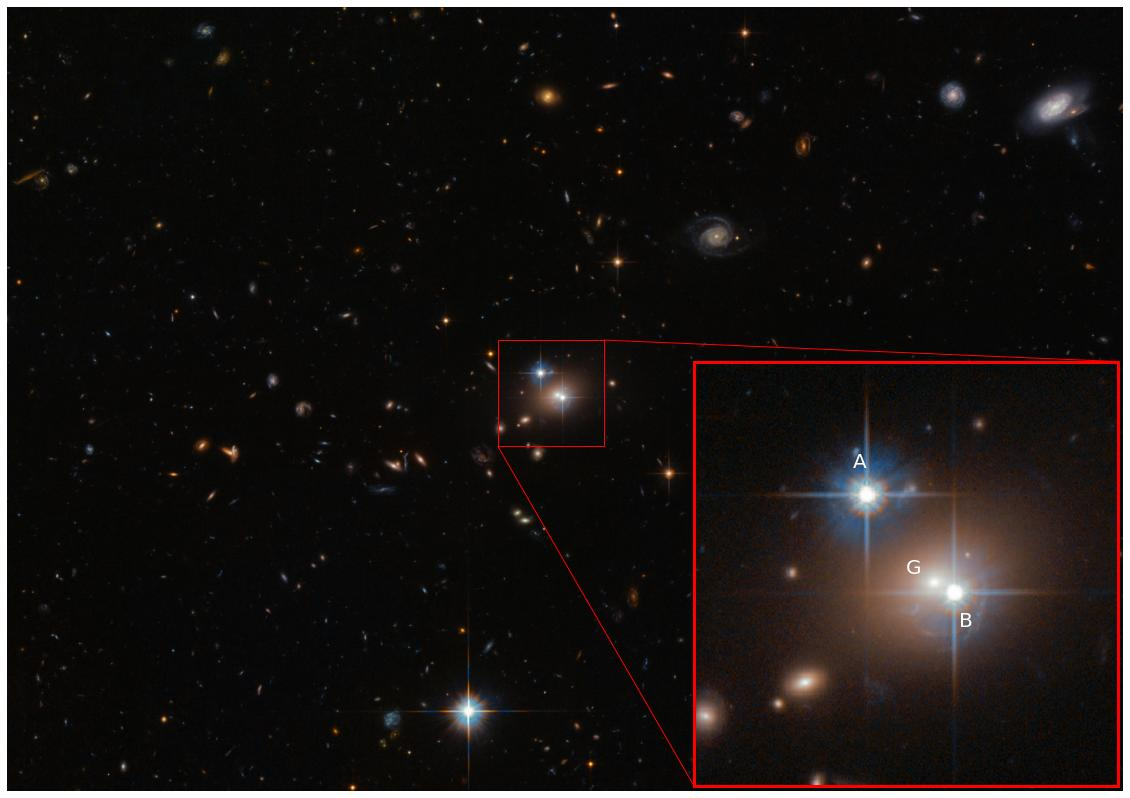
\includegraphics[width=0.8\textwidth]{figures/zoomed_in_qso0957}
        \caption{Le quasar double (QSO 0957+561 A et B) et la galaxie-lentille (G) imagée par le télescope spatial Hubble. 
        Crédit: ESA/Hubble et NASA, enlargissement par AA.}
        \label{fig:doubel quasar}
\end{figure}

Dû à cette difficulté pratique, 
la première lentille gravitationnelle est découverte seulement plusieurs décennies après la prédiction de leur existence par \citet{Walsh1979}, 
suivant l'identification de deux spectres radios de quasars identiques, QSO 0957+561 A et B, séparés par $5.7$ secondes d'arcs
et capturés avec le télescope radio Mark II à l'observatoire Jodrell Bank. 
Les spectres partagent la même magnitude, $m=17$, le même décalage vers le rouge, $z=1.405$, et possèdent des détails 
chimiques suspicieusement semblables. Ces coïncidences suggèrent fortement que ces deux spectres sont des copies d'un seul objet, soit un noyau 
actif d'une galaxie en arrière-plan, produite par l'effet de lentille gravitationnelle d'une galaxie en avant-plan, invisible dans le 
domaine radio à une fréquence de $966\,\mathrm{MHz}$. Cette hypothèse est rapidement confirmée par 
l'observation optique de la galaxie-lentille ($z=0.355$) avec l'observatoire Palomar \citep{Young1980}\footnote{Simulténament 
observé et confirmé par le télescope de $2.2\, m$ de l'Université d'Hawaii au mont Mauna Kea \citep{Stockton1980}.}, 
ainsi que la modélisation de sa distribution de masse, de son environnement 
et des angles de déflexion qui causeraient l'apparition d'une image double du quasar \citep{Young1981,Falco1991}

À la suite de cette découverte fortuite, l'étude des lentilles gravitationnelles est devenue un sujet d'étude 
particulièrement riche et prometteur pour la cosmologie \citep{Blandford1992,Bartelmann2010,Treu2010}. 
Par exemple, les lentilles gravitationnelles permettent de mesurer 
la constante de \citet{Hubble1929}, $H_0$, qui mesure le taux de l'expansion de l'Univers au temps présent. Les deux méthodes principales 
pour faire cette mesure à l'aide des lentilles gravitationnelles sont la caractérisation de la courbe de lumière des supernovas lentillées 
\citep{Refsdal1964,Kelly2015,Goobar2017} 
et la surveillance décennale de quasars lentillés 
\citep[e.g.][]{Vanderriest1989,Wong2020}. 



\begin{figure}[tb!]
        \centering
        \begin{subfigure}[t]{0.45\textwidth}
                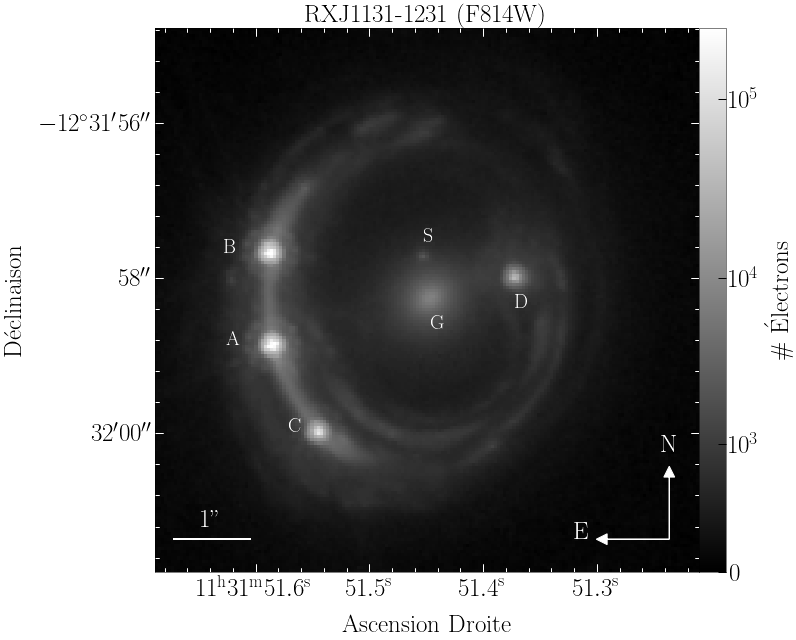
\includegraphics[width=\linewidth]{figures/rxj1131} 
                \caption{Quasar quadruplement lentillé (A, B, C et D) par une galaxie (G). L'image de la galaxie hébergeant le quasar 
                        est déformée tangentiellement, formant un anneau d'Einstein. Image prise par HST avec le filtre F814W.}
                \label{fig:rxj1131}
        \end{subfigure}
        ~
        \begin{subfigure}[t]{0.45\textwidth}
                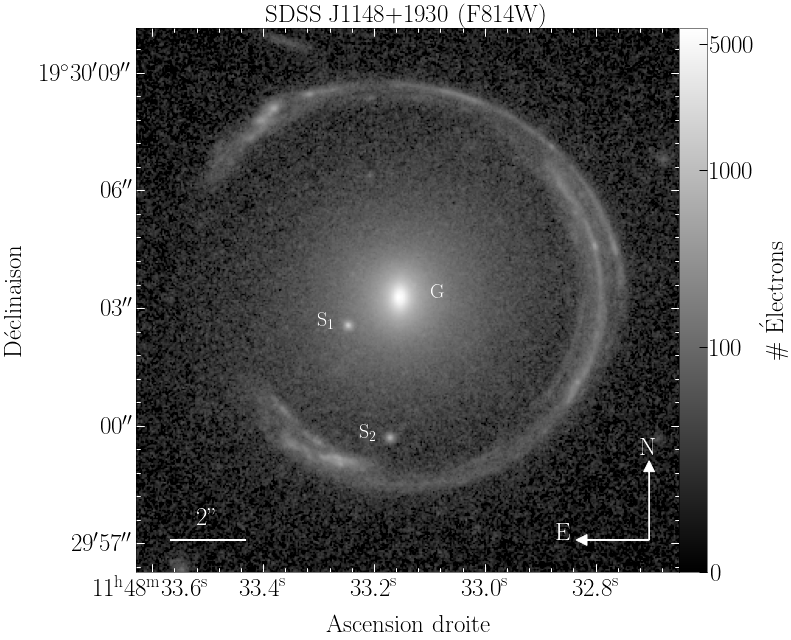
\includegraphics[width=\linewidth]{figures/sdssj1148} 
                \caption{Le fer à cheval cosmique, soit l'image d'une proto-galaxie à très haut décalage vers le rouge 
                        ($z=2.379$) fortement magnifiée et déformée par une galaxie elliptique lumineuse en infrarouge (G) exceptionnellement massive 
                        \citep[${5.2\times 10^{12}\, h_{72}^{-1}\, M_\odot}$,][]{Schuldt2019}. 
                 Image prise par HST avec le filtre F814W.}
                \label{fig:sdssj1148}
        \end{subfigure}
        \caption{Lentilles gravitationnelles de type galaxie-galaxie.}
        \label{fig:important lenses}
\end{figure}
 

De ce fait, plusieurs programmes ont été entamés pour trouver des lentilles gravitationnelles. Le programme 
\textit{Sloan Lens ACS Survey} \citep[SLAC,][]{Bolton2005,Bolton2006}, basé sur la recherche systématique de spectres de galaxies de type ETG\footnote{\textit{Early-Type Galaxies}} 
avec des lignes d'absorption à un décalage vers le rouge plus grand que les lignes d'émission, 
est un des programmes les plus réussis, ayant mené à la découverte 
confirmée de plus de $150$ lentilles gravitationnelles de type galaxie-galaxie \citep{Bolton2008,Shu2017}. Les programmes 
basés sur la recherche visuelle d'images doubles, triples, d'arcs ou d'anneaux \citep[e.g.][]{Faure2008} dans les champs larges et profonds comme 
COSMOS \citep{Koekemoer2007,Scoville2007}, connaissent aujourd'hui une renaissance nourrie par les succès récents de l'apprentissage profond 
pour la perception visuelle \citep{Krizhevsky2012}. Cette nouvelle approche a déjà mené à la découverte de plus de $1000$ lentilles 
gravitationnelles \citep{Petrillo2017,Huang2021}, et est projetée de découvrir plus de $10^{5}$ systèmes grâce aux nouvelles expéditions 
à champs larges comme les observatoires Rubin \citep{lsst2009} et Euclid \citep{Euclid2010}.


Le sujet du chapitre \ref{chap:censai} se concentre sur le défi de développer un algorithme pour modéliser la distribution de masse et 
la morphologie de la source. Cet algorithme est dédié à analyser le nombre grandissant
de lentilles gravitationnelles connues, dans toute leur complexité et dans un temps à l'échelle humaine. 
Dans la section qui suit, je dérive les équations centrales qui nous permettent 
d'étudier les lentilles gravitationnelles de type galaxie-galaxie.
Mon traitement est largement inspiré 
des manuels de références de \citet{Meneghetti2013,Congdon2018}. 


\subsection{Les angles de déflexion}

Supposons qu'un photon est sur une trajectoire parallèle à l'axe de 
visée $\mathbf{e}_{\parallel}$ d'un observateur sur Terre. 
Supposons de plus que la source d'un champ gravitationnel $\Phi$ est située sur l'axe de visée, 
ce qui a pour effet de courber la 
trajectoire de ce photon entre son point d'origine $A$ et son point d'arrivée $B$.
On définit l'angle de déviation comme la déviation totale de cette trajectoire 
dans la direction perpendiculaire à l'axe de visée de l'observateur. 
De façon générale, cette déviation s'écrit
\begin{equation}\label{eq:intro alpha}
        \boldsymbol{ \alpha} = - \int_{\lambda_A}^{\lambda_B} \ddot{\mathbf{x}} \times \mathbf{e}_{\parallel} d\lambda\, ,
\end{equation}
où $\lambda$ paramétrise la trajectoire du photon $\mathbf{x}(\lambda)$. 
Le signe négatif nous indique qu'on prend la perspective de l'observateur. 

La trajectoire d'un photon obéit au 
principe de Fermat, qui stipule que la lumière suit une trajectoire qui extrémise
la durée du parcours entre deux points. 
Dans le langage du calcul 
des variations, la variation de la durée s'écrit
\begin{equation}\label{eq:Fermat}
        \delta T =  \delta \int_{A}^{B} n(\mathbf{x}(\ell)) \frac{d\ell}{c}= 0\, ,
\end{equation}
où $\ell$ est un élément de longueur sur la trajectoire et $n$ est un indice de réfraction.
Pour déterminer l'indice de réfraction du champ gravitationnel d'une galaxie, 
on doit utiliser le formalisme de la relativité générale. Selon le principe 
d'équivalence (fort), 
l'effet d'un champ gravitationnel est localement 
indistinguable d'une accélération causée par la courbure 
d'un espace-temps décrit par 
une métrique $g_{\mu \nu}$. 
La trajectoire d'un photon se trouve alors en cherchant 
les géodésiques de cet espace-temps. 
On fait l'approximation 
que le potentiel $\Phi$ d'une galaxie est celui d'un gaz parfait, c'est-à-dire 
qu'il satisfait une équation de Poisson
\begin{equation}\label{eq:Poisson}
       \grad^{2}\Phi = 4\pi G \rho .
\end{equation} 
Dans la limite où ce potentiel est faible $\displaystyle \frac{2\Phi}{c^{2}} \ll 1$, la 
métrique $g_{\mu \nu}$ est décrite par une expansion au premier ordre autour de la 
métrique de Minkowsky %$\eta_{\mu\nu}$
\begin{equation}\label{eq:metrique}
        ds^2 = g_{\mu\nu}dx^{\mu}dx^{\nu} \approx \left( 1 + \frac{2\Phi}{c^{2}} \right)c^{2}dt^{2} - \left( 1 - \frac{2\Phi}{c^{2}} \right)d\mathbf{x}^{2}.
\end{equation} 
Puisqu'un photon suit une géodésique de l'espace-temps $ds^{2} = 0$, on peut déterminer 
l'indice de réfraction en réarrangeant l'équation \eqref{eq:metrique}
\begin{equation}\label{eq:n}
        n \equiv c \left( \frac{\lVert d \mathbf{x} \rVert}{dt}  \right)^{-1} \approx  1 - \frac{2\Phi}{c^{2}}.
\end{equation} 
En réécrivant l'élément de longueur $d\ell$ en termes du 
paramètre de la trajectoire
$
        d\ell = \left\lVert\frac{d  \mathbf{x} }{d\lambda} \right\rVert d\lambda,
$
on peut réécrire l'équation \eqref{eq:Fermat} sous la forme
\begin{equation}\label{eq:Fermat2}
        \delta \int_{\lambda_A}^{\lambda_B} n(\mathbf{x}) \lVert \mathbf{\dot{x}} \rVert d\lambda = 0.
\end{equation} 
Par correspondance avec la fonctionnelle de l'action 
$J(x) = \int_{\lambda_0}^{\lambda_1} \mathcal{L}(\lambda,\, x,\,\dot{x}) d\lambda$, on trouve que 
le lagrangien de la trajectoire s'écrit 
$
        \mathcal{L} = n(\mathbf{x})  \sqrt{\dot{x}^{2}}.
$
La trajectoire qui satisfait \eqref{eq:Fermat} 
est une solution des équations d'Euler-Lagrange
\begin{equation}\label{eq:EulerLagrange}
        \frac{d }{d \lambda} \frac{\partial \mathcal{L}}{\partial \dot{\mathbf{x}}} - \frac{\partial \mathcal{L}}{\partial \mathbf{x}} = 0.
\end{equation} 
On a donc
\begin{equation}\label{eq:EulerLagrange2}
        \frac{d }{d \lambda} n \frac{\dot{\mathbf{x}}}{\lVert \dot{\mathbf{x}} \rVert}- \lVert \dot{\mathbf{x}} \rVert \grad n = 0 ,
\end{equation} 
Puisque le choix du paramètre $\lambda$ est libre, on peut le choisir tel 
que $\lVert \dot{\mathbf{x}} \rVert = 1$ en tout point de la trajectoire. Ainsi,
\begin{align}
        \nonumber
        \frac{d }{d \lambda} n \dot{\mathbf{x}} -  \grad n &= 0 \\
\label{eq:EulerLagrange3}
        \implies n \ddot{\mathbf{x}} + (\grad n \cdot \dot{\mathbf{x}}) \dot{\mathbf{x}} - \grad n &= 0
\end{align} 

À ce point de la dérivation, on utilise l'approximation de Born. 
C'est-à-dire qu'on approxime la trajectoire 
du photon comme une ligne droite sur l'axe de visée $\mathbf{e}_{\parallel}$. 
Cette approximation est justifiée 
dans le contexte des lentilles gravitationnelles de type galaxie-galaxie, 
puisque les angles de déviation sont généralement de 
l'ordre de l'arcseconde ou plus petit. 
Comme le vecteur $\dot{\mathbf{x}}$ est tangent à la trajectoire du photon, les termes $ \propto \dot{\mathbf{x}} \times \mathbf{e}_{\parallel} $ s'annulent. 
En subsitutuant l'indice de réfraction par \eqref{eq:n} dans $\mathbf{e}_{\parallel} \times \eqref{eq:EulerLagrange3}$, on obtient
\begin{equation}\label{eq:sol}
        \ddot{\mathbf{x}} \times \mathbf{e}_{\parallel} = \frac{1}{n} \grad_\perp n = \grad_\perp \log n
        \approx -\frac{2}{c^{2}}\grad_{\perp} \Phi\,,
\end{equation} 
où $\grad_\perp$ est un gradient selon les coordonnées perpendiculaires à $\mathbf{e}_\parallel$.
On note que le facteur 2 qui apparaît dans l'équation \eqref{eq:sol} est un 
effet qui vient de la relativité générale. Ce facteur corrige la solution 
que l'on aurait obtenue avec une dérivation classique (newtonienne).


On est maintenant en mesure de calculer l'angle de déviation. 
J'introduis le paramètre d'impact $\boldsymbol{\xi}$ qui est la distance perpendiculaire entre 
la position d'origine du photon sur le plan de la lentille  
et l'axe de visée (voir Figure \ref{fig:cartoon}).
Dans le cas où le potentiel est généré par une masse $M$ ponctuelle, c.-à-d.\ qu'on 
suppose $\rho = M\delta^{3}(\mathbf{x})$, où $\delta $ est la fonction delta de Dirac, 
alors le potentiel qui satisfait l'équation de Poisson \eqref{eq:Poisson} est 
la fonction de Green 
$\displaystyle \Phi = -\frac{GM}{\sqrt{ \xi^{2} + z^{2}}}$, où $z$ est la coordonnée 
sur l'axe de visée. L'équation \eqref{eq:intro alpha} se réécrit finalement comme 
\begin{align}
\nonumber
        \boldsymbol{ \alpha}(\boldsymbol{ \xi} ) &= -\frac{2GM}{c^{2}} \int_{-\infty }^{\infty }  \frac{\partial}{\partial \boldsymbol{\xi} }\frac{1}{(\xi^{2} + z^{2})^{1/2}}dz \\
\label{eq:deflection approx}
        \implies \boldsymbol{ \alpha}(\boldsymbol{ \xi})  &= \frac{4GM}{c^{2}  \xi^{2} } \boldsymbol{ \xi}
\end{align} 
Cette solution se généralise naturellement à un profil de masse quelconque en assumant 
qu'il s'exprime comme une somme d'éléments de masse $dm = \Sigma d^{2}\boldsymbol{ \xi}'$, 
où $\Sigma = \int \rho dz$ est une densité surfacique de masse. 
L'angle de déviation total mesuré à un point $\boldsymbol{\xi} $ est alors une convolution 
sur tout le plan de la lentille (mince) puisque l'équation \eqref{eq:deflection approx} dépend 
linéairement de la masse $M$:
\begin{equation}\label{eq:alpha physique}
        \boldsymbol{ \alpha} (\boldsymbol{ \xi} ) = \frac{4 G}{c^{2}} 
        \int_{\mathbb{R}^{2}} \Sigma (\boldsymbol{ \xi} ')
        \frac{\boldsymbol{ \xi}  - \boldsymbol{ \xi} '}{\lVert \boldsymbol{ \xi}  - \boldsymbol{ \xi} ' \rVert^{2}}d^{2}\boldsymbol{ \xi} '
\end{equation} 

\begin{figure}[tb!]
        \centering
        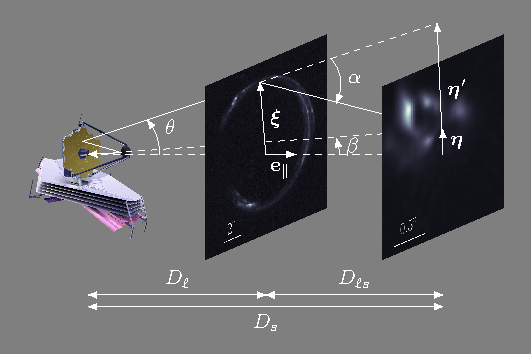
\includegraphics[width=0.8\textwidth]{figures/lensing_cartoon}
        \caption{Schéma d'une lentille gravitationnelle.}
        \label{fig:cartoon}
\end{figure}

L'angle de déviation est une quantité cruciale pour résoudre une lentille gravitationnelle 
puisqu'il décrit une transformation des coordonnées angulaires du plan de la lentille ($\boldsymbol{ \theta} $) 
vers les coordonnées angulaires du plan de la source ($\boldsymbol{ \beta} $). 
On assume que les distances entre l'observateur et la lentille $D_{\ell}$, entre l'observateur et la source $D_s$ et entre la lentille et la source $D_{\ell s}$, 
sont beaucoup plus grandes que les distances perpendiculaires à l'axe de visée $\boldsymbol{ \xi} $ ou $\boldsymbol{ \eta}$ 
(voir figure \ref{fig:cartoon}). 
Cette approximation est justifiée pour les objets qui nous intéressent,
pour lesquels les distances parallèles à l'axe de visée sont généralement 
de l'ordre du Gpc, alors que les distances perpendiculaires sont généralement 
de l'ordre du kpc; soit 6 ordres de grandeur de différence.
Ainsi, on peut faire un argument géométrique (euclidien) 
\begin{align}
\nonumber
       D_{s} \boldsymbol{ \theta} &= \boldsymbol{ \eta}' \\   
\nonumber
       D_{s} \boldsymbol{ \beta} &= \boldsymbol{ \eta} \\   
\nonumber
       D_{\ell s} \boldsymbol{ \alpha} &= \boldsymbol{ \eta}' - \boldsymbol{ \eta}  \\   
\label{eq:lens equation}
       \implies D_s \boldsymbol{ \beta} &= D_s \boldsymbol{ \theta} - D_{\ell s} \boldsymbol{ \alpha}   
\end{align} 
La dernière relation est l'équation maîtresse qui nous permet de tracer les rayons lumineux d'une source 
vers un détecteur fictif dans nos simulations. 

On notera que cette relation reste valide pour un Univers courbe et/ou en expansion 
(c.-à-d.\ décrit par une géométrie non euclidienne), 
à condition qu'on utilise une notion de distance qui satisfait, par définition, la relation trigonométrique euclidienne
\begin{equation}\label{eq:diameter angular distance}
       D \equiv \frac{\xi}{\theta}\, ,
\end{equation} 
où $\xi$ est la taille physique d'un objet placé à une certaine distance de l'observateur, et $\theta$ est l'angle solide sous-tendu 
par cet objet. Pour un Univers décrit par la métrique de Friedmann-Lemaître-Robertson-Walker,
la notion de distance qui respecte la définition \eqref{eq:diameter angular distance} est la distance du diamètre angulaire. 
En pratique, on peut exprimer $D$ en termes du décalage vers le rouge des photons émis par l'objet, $z$. 
On note $a(z)$ le facteur d'échelle lorsque le photon est émis par la source et $a(0)$ le facteur d'échelle au moment présent ($z=0$).
Pour un Univers plat \citep[voir les manuels de référence][]{Coles2002,Dodelson2003,Bartelmann2004}
\begin{align}
        D_z &= c a(z) \underbrace{\int_{a(z)}^{a(0)} \frac{da}{a \dot{a}}}_{\strut\mathclap{\text{distance comobile}}}; \\[2ex]
                \nonumber
              &= \frac{c a(z)}{H_0} \int_{a(z)}^{a(0)} \frac{da}{\sqrt{\Omega_{r,0} + \Omega_{m,0} a  + \Omega_{\Lambda,0}a^{4}}}; \\
              \label{eq:dang}
              &= \frac{c}{H_0(1 + z)} \int_{0}^{z} \frac{dz'}{\sqrt{\Omega_{r,0}(1 + z')^{4} + \Omega_{m,0} (1 + z')^{3} + \Omega_{\Lambda,0} }}\, .
\end{align}
On a utilisé la relation entre le facteur d'échelle, $a$, et le décalage vers le rouge, $a = (1 + z)^{-1}$, pour obtenir l'équation \eqref{eq:dang} 
par un changement de la variable d'intégration. 
$\Omega_{r,0}$, $\Omega_{m,0}$ et $\Omega_{\Lambda, 0}$ sont les paramètres de densités, au temps présent, de la radiation, de la matière et de l'énergie sombre 
respectivement. 
%$\Omega_K = 1 - \Omega_0$ est le paramètre de courbure et 
$H_0$ est la constante de Hubble, soit le taux 
d'expansion de l'Univers au temps présent. La distance $D_{\ell s}$ se trouve simplement en ajustant les bornes de l'intégrale $\int_0^{z} \mapsto \int_{z_\ell}^{z_s}$.
La valeur des paramètres du modèle cosmologique $\Lambda$CDM obtenue par l'équipe \citet{PlanckCollaboration2018}
est rapportée dans l'annexe \ref{app:lcdm}.


Il est généralement pratique de travailler avec la forme adimensionnelle de l'équation \eqref{eq:lens equation}. 
On introduit la densité critique 
\begin{equation}\label{eq:densite critique}
        \Sigma_c = \frac{c^2}{4 \pi G}\frac{D_{s}}{D_{\ell s} D_\ell}\, ,
\end{equation} 
qui nous permet de définir la quantité qu'on nomme convergence $\displaystyle \kappa(\boldsymbol{ \theta} ) \equiv \frac{\Sigma(\boldsymbol{ \theta})}{\Sigma_c}$. 
On définit ainsi l'angle réduit 
\begin{equation}\label{eq:alpha adim}
        \hat{\boldsymbol{ \alpha}} (\boldsymbol{ \theta}) = \frac{1}{\pi}\int_{\mathbb{R}^{2}} \kappa(\boldsymbol{ \theta} )
        \frac{\boldsymbol{ \theta} - \boldsymbol{ \theta}'  }{\lVert \boldsymbol{ \theta} - \boldsymbol{ \theta}' \rVert  } d^{2}\boldsymbol{ \theta}'\, ,
\end{equation} 
qui satisfait l'équation de la lentille adimensionnelle 
\begin{equation}\label{eq:lens equation adim}
        \boldsymbol{ \beta} = \boldsymbol{ \theta} - \hat{\boldsymbol{ \alpha}}(\boldsymbol{ \theta})\, . 
\end{equation}


\section{Auto-encodeur variationnel}\label{sec:vae}
 
\subsection{Description du modèle}

Les auto-encodeurs variationnels (VAE) ont été introduits par \citet{Kingma2013} comme une approche 
pour inférer approximativement les variables latentes (ou cachées) qui contrôlent un certain processus génératif. 
Leur utilité est particulièrement marquée lorsque ce processus génératif est défini implicitement par un échantillon de données, 
soit un cas où la forme fonctionnelle de la distribution n'est pas connue a priori.
Dans cette section, j'introduis 
les concepts principaux reliés à ce type de modélisation. 
Le lecteur peut aussi se référer au livre blanc de \citet{Kingma2019}.

On définit $\mathbf{z}\in \mathbb{R}^{h}$ comme une variable latente et $\mathbf{x}\in \mathbb{R}^{m}$ ($m > h$) 
comme un exemple d'un échantillon de donnée $\mathcal{D} = \{\mathbf{x}^{(i)}\}_{i=1}^{N}$. 
Notre objectif est de modéliser la distribution, $p(\mathbf{x})$, implicitement décrite par notre échantillon. 
On définit une approximation de cette distribution, $p_\theta(\mathbf{x})$, caractérisée par une liste de paramètres $\theta$,
et on définit un processus génératif modélisé par la conditionnelle sur la variable cachée $p_\theta(\mathbf{x \mid \mathbf{z}})$. 
Déterminer $p_\theta$ directement est généralement difficile, voir impossible, si la dimensionnalité de $\mathbf{x}$ est grande 
($\mathrm{dim(\mathbf{x}}) \gtrsim 10^{4}$ pour des images). 
Pour contourner ce problème, on introduit une distribution variationnelle, $q_\phi(\mathbf{z} \mid \mathbf{x})$, dont le rôle est 
d'inférer la variable latente $\mathbf{z}$ associée à $\mathbf{x} \sim p_\theta(\mathbf{x} \mid \mathbf{z})$. 
En d'autres mots, $q_\phi(\mathbf{z} \mid \mathbf{x})$ est une approximation variationnelle de la distribution a posteriori $p_\theta(\mathbf{z} \mid \mathbf{x})$.
La notion de distance entre ces deux distributions est mesurée par la divergence de Kullback-Leibler $D_{\mathrm{KL}}(\cdot \KL \cdot) \geq 0$: 
\begin{align}
        \nonumber
       D_{\mathrm{KL}}(q_\phi(\mathbf{z} \mid \mathbf{x}) \KL  p_\theta (\mathbf{z} \mid \mathbf{x})) 
       &= \mathbb{E}_{q_\phi(\mathbf{z} \mid \mathbf{x})} \bigg[\log q_\phi(\mathbf{z} \mid \mathbf{x}) - \log p_\theta (\mathbf{z} \mid \mathbf{x}) \bigg]  \\
       \nonumber
       &= \mathbb{E}_{q_\phi(\mathbf{z} \mid \mathbf{x})} \bigg[\log q_\phi (\mathbf{z} \mid \mathbf{x}) -\log \frac{p_\theta(\mathbf{z}, \mathbf{x})}{p_\theta(\mathbf{x})} \bigg]  \\
       \label{eq:KL}
       &= \log p_\theta (\mathbf{x}) - \underbrace{\mathbb{E}_{q_\phi(\mathbf{z} \mid \mathbf{x})} \bigg[\log p_\theta(\mathbf{z}, \mathbf{x}) - \log q_\phi (\mathbf{z} \mid \mathbf{x}) \bigg]}_{\equiv \mathcal{L}_{\phi,\theta}(\mathbf{x})} \, .
\end{align} 

On remarque par cette manipulation que la distance $D_{\mathrm{KL}}$, en plus de mesurer la distance entre 
les deux distributions a posteriori (par définition), mesure aussi la différence entre le terme 
$\mathcal{L}_{\phi,\theta}(\mathbf{x})$, qu'on nomme limite inférieure sur l'évidence (de l'anglais 
\textit{evidence lower bound}: ELBO), et la distribution marginale qu'on cherche à modéliser, $p_\theta(\mathbf{x})$. 
L'objectif d'un modèle VAE est de maximiser la ELBO, $\mathcal{L_{\phi,\theta}}$. 
En observant l'équation \eqref{eq:KL}, on réalise que cet objectif 
nous permet d'améliorer le modèle d'inférence et le processus génératif simultanément.
En effet, la divergence KL est 
une quantité positive, donc maximiser la ELBO a pour effet de
\begin{enumerate}
        \item maximiser $p_\theta(\mathbf{x}) = \int p_{\theta}(\mathbf{x} \mid \mathbf{z}) p_{\theta}(\mathbf{z}) d\mathbf{z}$, ce qui suit de l'inégalité
                $\log p_\theta \geq \mathcal{L}_{\phi,\theta}(\mathbf{x})$ (améliore le processus génératif);
        \item minimiser $D_{\mathrm{KL}}(q_\phi(\mathbf{z} \mid \mathbf{x}) \KL  p_\theta (\mathbf{z} \mid \mathbf{x})) = \log p_\theta(\mathbf{x}) - \mathcal{L}_{\phi,\theta}(\mathbf{x})$ (améliore le processus d'inférence de $\mathbf{z}$).
\end{enumerate}

\begin{figure}[H]
        \centering
        \begin{tikzpicture}
                \node[circle, draw=black, minimum size=1cm] (z) at (0, 3) {$\mathbf{z}$};
                \node[circle, draw=black, minimum size=1cm] (x) at (0, 0) {$\mathbf{x}$};
                \draw[-{Latex[scale=2]}] (z) to (x);
                \draw[-{Latex[scale=2]}, in=225, out=135, dashed] (x) to (z);
                \node (phi) at (-2.5, 2.5) {$\phi$};
                \node (theta) at (2.5, 2.5) {$\theta$};
                \draw[rounded corners=0.5cm] (-1.5, -0.7) rectangle (1.5, 3.7);
                \draw[-{Latex[scale=2]}] (theta) to node[sloped, midway, below=5pt, fill=white, rectangle, draw=white, opacity=.8, text opacity=1] {$p_\theta(\mathbf{\mathbf{x} \mid \mathbf{z}})$} (x);
                \draw[-{Latex[scale=2]}] (theta) to node[sloped, midway, above=5pt, fill=white, rectangle, draw=white, opacity=.8, text opacity=1] {$p_\theta(\mathbf{z})$} (z);
                \draw[-{Latex[scale=2]}, dashed] (phi) to node[sloped, midway, above=5pt, fill=white, rectangle, draw=white, opacity=.8, text opacity=1] {$q_\phi(\mathbf{z} \mid \mathbf{x})$} (z); 
                \node at (1, -0.5) {$N$};
        \end{tikzpicture}
        \caption{Modèle graphique d'un VAE. Les flèches pleines indiquent le processus génératif, alors que les flèches pointillées indiquent le processus d'inférence.}
        \label{fig:vae encoder}
\end{figure}

\subsection{Le truc de reparamétrisation}
Le gradient de la ELBO par rapport aux paramètres variationnels, $\grad_{\phi,\theta}\mathcal{L}_{\phi,\theta}(\mathbf{x})$, 
est une quantité qu'on doit calculer pour faire usage d'algorithmes comme la grimpe de gradient stochastique 
pour maximiser la ELBO en termes de $\phi$ et $\theta$. 
Or, la liste de paramètres $\phi$ apparait dans la distribution de prélèvement pour calculer 
l'espérance mathématique $\mathbb{E}_{q_\phi(\mathbf{z} \mid \mathbf{x})}$ dans la ELBO \eqref{eq:KL}.
Cette opération n'a pas de dérivée formelle en termes de $\phi$. 

Pour résoudre ce problème, on utilise le truc de reparamétrisation \citep{Kingma2013}, 
qui consiste à exprimer la variable aléatoire latente $\mathbf{z} \sim q_\phi (\mathbf{z} \mid \mathbf{x})$ 
comme la transformation différentiable et inversible d'une variable aléatoire auxiliaire $\boldsymbol{\epsilon}$.
On considère le cas où $q_\phi(\mathbf{z} \mid \mathbf{x})$ et $p(\boldsymbol{ \epsilon})$ 
font partie de la famille gaussienne isotropique
\begin{align}
        \label{eq:p epsilon}
        \boldsymbol{\epsilon} &\sim \mathcal{N}(0, \bbone)\, ;\\
        %\label{eq:q phi}
        %q_\phi(\mathbf{z} \mid \mathbf{x}) &= \mathcal{N}(\boldsymbol{ \mu}_\phi (\mathbf{x}),\, \bbone \boldsymbol{\sigma}_\phi^{2}(\mathbf{x}))\, ;\\
        \label{eq:reparametrisation}
        \mathbf{z} &= \boldsymbol{\mu}_\phi + \boldsymbol{ \sigma}_\phi \odot \boldsymbol{ \epsilon}\, , 
\end{align} 
de sorte que 
\begin{equation}\label{eq:q phi}
        \mathbf{z} \sim q_\phi(\mathbf{z} \mid \mathbf{x}) = \mathcal{N}(\boldsymbol{ \mu}_\phi (\mathbf{x}),\, \bbone \boldsymbol{\sigma}_\phi^{2}(\mathbf{x}))\, .
\end{equation} 
$\odot$ symbolise le produit d'Hadamard, ou encore le produit élément par élément de vecteurs.
La reparamétrisation fait en sorte que les paramètres variationnels ne participent plus au processus de prélèvement, 
maintenant pris en charge par $\boldsymbol{ \epsilon} $.
Cette propriété est cruciale, car elle nous permet de prendre le gradient de la ELBO \eqref{eq:KL}. 
En effet, on peut maintenant échanger les opérateurs $\grad_{\phi,\theta}$ et ${\mathbb{E}_{q_\phi(\mathbf{z} \mid \mathbf{x})} = \mathbb{E}_{p(\boldsymbol{ \epsilon})}}$,
ce qui nous permet d'appliquer le gradient à l'intérieur de l'espérance mathématique.
De plus, $\phi$ décrit maintenant une fonction générique dont le rôle est d'inférer les 
paramètres de la distribution $q_\phi(\mathbf{z} \mid \mathbf{x})$
\begin{equation}
        \begin{aligned}
                f_\phi: \mathbb{R}^{m} &\rightarrow \mathbb{R}^{h} \times \mathbb{R}^{h}\\ \mathbf{x} &\mapsto (\boldsymbol{\mu},\, \log \boldsymbol{\sigma}^{2})
        \end{aligned}
\end{equation} 
En pratique, on peut construire une approximation de 
cette fonction avec un réseau de neurones convolutif lorsque $\mathbf{x}$ est une image, 
suivant le principe d'approximation universelle \citep{Cybenko1989,Hornik1991}. 

L'objectif d'entraînement de la fonction $f_\phi$ nécessite de manipuler la ELBO pour obtenir une 
divergence KL
\begin{align}
        \mathcal{L}_{\phi,\theta}(\mathbf{x}) &= \mathbb{E}_{q_\phi(\mathbf{z} \mid \mathbf{x})} \bigg[ \log p_\theta(\mathbf{z}, \mathbf{x}) - \log q_\phi (\mathbf{z} \mid \mathbf{x}) \bigg]\, ; \\
        \label{eq:final elbo}
         \implies \mathcal{L}_{\phi,\theta}(\mathbf{x})  &= 
         \underbrace{\mathbb{E}_{q_\phi(\mathbf{z} \mid \mathbf{x})} \bigg[ \log p_\theta(\mathbf{x} \mid \mathbf{z})\bigg]}_{\text{terme de reconstruction}}
         + \underbrace{
                \mathbb{E}_{q_\phi(\mathbf{z} \mid \mathbf{x})} \bigg[\log p_{\theta}(\mathbf{z}) - \log q_\phi (\mathbf{z} \mid \mathbf{x}) \bigg]
        }_{\equiv -D_{\mathrm{KL}}(q_\phi(\mathbf{z} \mid \mathbf{x})\, \KL\, p_\theta(\mathbf{z}))}\, .
\end{align} 
Pour déterminer la forme fonctionnelle de la divergence KL obtenue au second terme du membre droit de l'équation \eqref{eq:final elbo}, 
on stipule a priori que la distribution marginale des variables latentes 
devrait correspondre à une distribution normale isotropique
\begin{equation}\label{eq:latent distribution}
        p_{\theta}(\mathbf{z}) = \mathcal{N}(0, \bbone)
\end{equation}
La KL admet alors une solution fermée étant donné les familles paramétriques stipulées 
pour $p_\theta(\mathbf{z})$ \eqref{eq:latent distribution} et $q_\phi(\mathbf{z} \mid \mathbf{x})$ \eqref{eq:q phi}
\begin{equation}\label{eq:final KL}
        -D_{\mathrm{KL}}(q_\phi(\mathbf{z} \mid \mathbf{x})\, \KL\, p_\theta(\mathbf{z})) =
        \frac{1}{2}\sum_{j=1}^{h} (1 + [\log \boldsymbol{ \sigma}_\phi^{2} ]_j - [\boldsymbol{ \mu}_\phi ]_j - [\boldsymbol{ \sigma}_\phi^{2} ]_j)
\end{equation} 
Une dérivation de ce terme est donnée dans l'annexe B de \citet{Kingma2013}. 
%Cette solution se dérive directement par rapport à $\phi$. 
Le premier terme du membre droit de l'équation \eqref{eq:final elbo} 
est nommé \textit{terme de reconstruction} puisqu'il connecte avec l'objectif des fonctions 
de type auto-encodeur d'apprendre une représentation latente d'un échantillon de données.
La reconstruction s'accomplit en utilisant d'abord le modèle d'inférence 
$\mathbf{z}^{(1:L)} \overset{\mathrm{i.i.d}}{\sim} q_\phi(\mathbf{z} \mid \mathbf{x})$ 
pour obtenir un échantillon de représentations latentes à partir des équations \eqref{eq:p epsilon} à \eqref{eq:reparametrisation}, 
puis en utilisant le modèle génératif $\hat{\mathbf{x}}^{(i)} \sim p_\theta(\mathbf{x} \mid \mathbf{z}^{(i)})$ pour obtenir 
un échantillon de reconstructions $\mathbf{\hat{x}}^{(1:L)}$ de l'exemple originel $\mathbf{\mathbf{x}}$. 
Comme on a déjà une variable auxiliaire $\boldsymbol{ \epsilon} $ 
qui se charge de l'aspect génératif du modèle, on peut construire une approximation du 
modèle génératif avec une fonction générique des variables latentes 
${g_\theta: \mathbb{R}^{h} \rightarrow \mathbb{R}^{m};\, \mathbf{z}^{(i)} \mapsto \hat{\mathbf{x}}^{(i)}}$.
Encore une fois, un réseau de neurones convolutif est un choix pratique pour modéliser cette fonction 
dans le cas où $\mathbf{x}$ est une image. En général, on choisit une erreur quadratique moyenne pour modéliser le terme de reconstruction, 
de sorte que
\begin{equation}\label{eq:reconstruction}
        \mathbb{E}_{q_\phi(\mathbf{z} \mid \mathbf{x})} \bigg[
                \log p_\theta(\mathbf{x} \mid \mathbf{z})
        \bigg] 
        = -\frac{1}{L}\sum_{i=1}^{L} \lVert \mathbf{x} - \hat{\mathbf{x}}^{(i)} \rVert_2^{2}
\end{equation} 

\subsection{Principe du goulot d'information}

La fondation théorique des auto-encodeurs variationnels repose sur le principe plus général 
du goulot d'information \citep[BIP, de l'anglais \textit{bottleneck information principle:}][]{Tishby1999}. 
Dans cette sous-section, je décris rapidement certains concepts 
liés à la théorie de l'information de \citet{Shannon1948} 
pour justifier l'introduction d'un multiplicateur de 
Lagrange $\beta$ au terme de régularisation de la ELBO, ${-D_{\mathrm{KL}}(q_\phi(\mathbf{z} \mid \mathbf{x})\, \KL\, p_\theta(\mathbf{z}))}$.
Pour une discussion en profondeur, voir l'excellente revue sur l'utilisation de BIP dans le contexte de l'apprentissage 
machine par \citet{Goldfield2020} et le manuel de référence sur la théorie de l'information par \citet{Cover2006}.
\begin{figure}[thb!]
        \centering
        \resizebox{\linewidth}{!}{
        \begin{tikzpicture}
                \node at (-8, -2.8) {Indice d'un};
                \node at (-8, -3.3) {ensemble des données};
                \node[circle, draw=black, minimum size=1cm] (obj) at (-8, -2) {$Y$}; 
                \node at (-8, 1.4) {Source};
                \node at (-8, 0.9) {d'information};
                \node[circle, draw=black, minimum size=1cm] (x) at (-8, 0) {$X$}; 
                \node at (-4, 1.3) {Encodeur};
                \node[rectangle, draw=black, minimum width=2cm, minimum height=2cm] (encoder) at (-4, 0) {$q_\phi(\mathbf{z} \mid \mathbf{x})$}; 
                \node at (0, 0.9) {Code};
                \node[circle, draw=black, minimum size=1cm] (z) at (0, 0) {$Z$};
                \node[circle, draw=black, minimum size=1cm] (eps) at (0, -2) {$\epsilon$};
                \node at (0, -2.8) {Source de bruit};
                \node[rectangle, draw=black, minimum width=2cm, minimum height=2cm] (decoder) at (4, 0) {$p_\theta(\mathbf{x} \mid \mathbf{z})$};
                \node at (4, 1.3) {Décodeur};
                \node[circle, draw=black, minimum size=1cm] (xhat) at (8, 0) {$\hat{X}$};
                \node at (8, 0.9) {Reconstruction};
               
                \draw[-latex] (obj) -- (x);
                \draw[-latex] (x) -- node[midway, below] {Message} (encoder);
                \draw[-latex] (encoder) -- node[midway, below] {Signal} (z);
                \draw[-latex] (z) -- node[midway, below] {Signal} (decoder);
                \node at (1.8, -0.8) {reçu};
                \draw[-latex] (decoder) --node[midway, below] {Message} (xhat);
                \node at (6.2, -0.8) {reçu};
                \draw[-latex] (eps) to (z);
        \end{tikzpicture}
}
        \caption{VAE comme un système de transmission d'information.}
        \label{fig:info VAE}
\end{figure}
L'objectif d'un auto-encoder est de construire un code $Z$ d'une longueur minimale qui capture un maximum d'information contenue dans un message $X$. 
Formellement, on utilise l'information mutuelle de Shannon pour mesurer l'information capturée par $Z$ à propos de $X$
\begin{equation}\label{eq:ShannonInfo}
        I(Z ; X) = D_{\mathrm{KL}}\left(p(\mathbf{x}, \mathbf{z}) \KL p(\mathbf{x}) p(\mathbf{z})\right) %= \mathbb{E}_{p(x,z)} \bigg[\log \frac{p(x,z)}{p(x) p(z)}\bigg] %= \sum_{x \in \mathcal{X}} \sum_{z \in \mathcal{Z}} p(x, z) \log \frac{p(x, z)}{p(x) p(z)}.
\end{equation} 
Il est utile de décomposer cet objectif en termes de l'entropie du message $H(X)$ et l'entropie 
conditionnelle de ce message étant donné le code $Z$, $H(X \mid Z)$
\begin{equation}\label{eq:info entropy}
       I(Z; X) = H(X) - H(X \mid Z) 
\end{equation} 
L'entropie est une mesure de l'incertitude dans une variable aléatoire
\begin{equation}\label{eq:entropy}
        H(X) = -\mathbb{E}_{p(\mathbf{x})}\big[\log p(\mathbf{x}) \big] \geq 0\, ,
\end{equation} 
qu'on interprète aussi comme une mesure de la longueur minimale d'un code, $Z$, pour 
transmettre un message, $X$, d'un émetteur à un receveur avec le minimum de perte d'information \citep{Shannon1948,Kolmogorov1965}.
L'entropie conditionnelle $H(X \mid Z)$ est une  mesure de l'incertitude résiduelle étant donné la connaissance du code $Z$. Dans le cas où $Z$ 
détermine complètement le message $X$, alors $H(X \mid Z) = 0$ et l'information mutuelle atteint son maximum $I(Z; X) = H(X)$.
Dans le cas où $Z$ et $X$ sont deux variables aléatoires indépendantes, $H(X \mid Z) = H(X)$ et l'information mutuelle devient nulle.

Déterminer l'auto-encodeur optimal, c.-à-d. celui qui maximise $I(Z;X)$, est un problème mal posé. 
En effet, on pourrait naïvement maximiser l'objectif \eqref{eq:ShannonInfo} avec 
la fonction identité comme auto-encodeur: $f_{\phi,\theta}(X) = \bbone X$, de sorte que $Z = X$ et $I(Z; X) = H(X)$. 
Or, $Z$ n'est pas une représentation pertinente dans ce cas. 
Pour éliminer les solutions non désirées, on introduit une contrainte sur la complexité de \citet{Kolmogorov1965} du code $Z$, c.-à-d. qu'on cherche 
un auto-encodeur qui compresse le message et conserve simultanément 
le maximum d'information possible à propos du message. On introduit l'objectif du goulot d'information \citep{Tishby1999}
\begin{equation}\label{eq:IB}
\begin{aligned}
        \underset{\phi,\theta}{\mathrm{max}}&\,\,I(Z ; X) \\[1ex]
        \text{sujet à}&\,\, I(Z; Y) \leq \alpha\, .
\end{aligned}
\end{equation} 
La contrainte $I(Z; Y) \leq \alpha$ impose à l'auto-encodeur %$p_{\phi,\theta}(\hat{X} \mid X)$
une limite sur l'information mutuelle entre le code 
utilisé pour représenter $X$ et l'identité $Y=i$ de chaque exemple d'un ensemble des données qu'on veut modéliser $\mathcal{D} = \{\mathbf{x}_i \}_{i=1}^{N}$.
Il s'avère que l'objectif de comprimer l'information est intimement lié à l'objectif d'obtenir un sommaire informatif, c.-à-d. qu'un 
code d'une complexité de \citet{Kolmogorov1965} minimale décrit la source d'information de la manière la plus informative possible. Cette connexion 
remarquable est une application concrète du principe du rasoir d'Occam: l'explication adéquate la plus simple est la meilleure explication.

Dans ce qui suit, je m'applique à redériver l'objectif d'un auto-encodeur variationnel suivant les approximations 
proposées par \citet{Alemi2017}. Puis, je termine avec une courte interprétation des VAE sous la lumière du principe du goulot d'information.
On commence par construire une limite variationnelle inférieure sur $I(Z; X)$. 
On assume d'abord la chaîne de Markov $Y \rightarrow X \rightarrow Z$ pour les variables 
aléatoires représentées dans la figure \ref{fig:info VAE}. La chaîne de Markov 
induit la factorisation de la probabilité jointe
\begin{equation}\label{eq:factorisation}
       p(X, Y, Z) = p(X \mid Z) p(Y \mid X) p(X) 
\end{equation} 
où $p(X \mid Z,\, Y) = p(X \mid Z)$ suit du fait que $Z$ et $Y$ sont des variables conditionnellement indépendantes étant donné $X$.
On introduit ensuite un modèle pour l'encodeur,
$q_\phi (Z \mid X)$, soit un système de transmission d'informations par compression. Il 
suit que 
\begin{align}
        I(Z;\, X) &\equiv \mathbb{E}_{p(\mathbf{z},\, \mathbf{x})} \bigg[\log \frac{p(\mathbf{x},\, \mathbf{z})}{p(\mathbf{x}) p(\mathbf{z})} \bigg]\, ;  \\[1.5ex]
        &= \mathbb{E}_{p(\mathbf{x})}\mathbb{E}_{q_\phi(\mathbf{z} \mid \mathbf{x})} \bigg[\log \frac{q_\phi(\mathbf{x} \mid \mathbf{z})}{p(\mathbf{x})} \bigg]\, ;  \\[1.5ex]
                &= -\mathbb{E}_{p(\mathbf{x})}\bigg[\log p(\mathbf{x}) \bigg]  
                + \mathbb{E}_{p(\mathbf{x})}\mathbb{E}_{q_\phi(\mathbf{z} \mid \mathbf{x})} \bigg[\log q_\phi(\mathbf{x} \mid \mathbf{z})\bigg]\, ;  \\[1.5ex]
                \label{eq:maximum info}
                \implies I(Z;\, X)&\geq \mathbb{E}_{p(\mathbf{x})}\mathbb{E}_{q_\phi(\mathbf{z} \mid \mathbf{x})} \bigg[\log p_\theta (\mathbf{x} \mid \mathbf{z})\bigg]\, .
\end{align}
À la dernière ligne, on a éliminé l'entropie du message $H(X)$, puisque c'est une constante strictement positive qui ne dépend pas de $\phi$.
On a aussi introduit l'approximation variationnelle $p_\theta (\mathbf{x} \mid \mathbf{z}) \approx q_\phi (\mathbf{x} \mid \mathbf{z})$ 
pour approximer la distribution a posteriori de l'encodeur (soit le décodeur). Cette approximation est valide dans le contexte où 
on cherche une limite inférieure pour $I(Z; X)$, puisque la divergence KL entre ces deux distributions est strictement positive.
Ensuite, on cherche une borne supérieure au terme de compression $I(Z; Y)$. 
Pour ce qui suit, on remplace $p(Y=i)$ par $\mathbf{x}^{(i)} \sim \mathcal{D}$ pour illustrer avec plus de clarté 
comment le processus génératif de l'indice induit une sélection d'un exemple $\mathbf{x}^{(i)}$ dans l'ensemble 
d'entraînement $\mathcal{D}$. Il suit que 
\begin{align}
        I(Z; Y) &= \mathbb{E}_{\mathbf{x}^{(i)} \sim \mathcal{D}} \mathbb{E}_{q_\phi(\mathbf{z} \mid \mathbf{x}^{(i)})} \bigg[ 
                \log \frac{q_\phi(\mathbf{z} \mid \mathbf{x}^{(i)}) }{q_\phi (\mathbf{z})}        
        \bigg]\, ; \\[1.5ex]
        \label{eq:compression}
        I(Z; Y) &\leq \mathbb{E}_{\mathbf{x}^{(i)} \sim \mathcal{D}} \mathbb{E}_{q_\phi(\mathbf{z} \mid \mathbf{x}^{(i)})} \bigg[ 
                \log \frac{q_\phi(\mathbf{z} \mid \mathbf{x}^{(i)}) }{p_\theta (\mathbf{z})}        
        \bigg]\, , 
\end{align}
où on a introduit l'approximation variationnelle $p_\theta(\mathbf{z}) \approx q_\phi(\mathbf{z})$. 
L'inégalité suit encore une fois 
du fait que la divergence KL entre ces deux distributions est strictement positive.
On finit la dérivation en écrivant l'objectif du goulot d'information \eqref{eq:IB} en introduisant un multiplicateur 
de Lagrange $\beta$ pour le terme $I(Z; Y)$ et en introduisant 
les limites variationnelles \eqref{eq:maximum info} et \eqref{eq:compression}. On ignore  
l'espérance mathématique $\mathbb{E}_{p(\mathbf{x})} = \mathbb{E}_{\mathbf{x}^{(i)} \sim \mathcal{D}}$ pour mieux illustrer la connexion 
avec la ELBO \eqref{eq:final elbo}
\begin{equation}\label{eq:beta VAE}
        \mathcal{L}_{\phi,\theta,\beta}(\mathbf{x}) =  \mathbb{E}_{q_\phi(\mathbf{z} \mid \mathbf{x})} \bigg[\log p_\theta (\mathbf{x} \mid \mathbf{z})\bigg]
        -  \beta  \mathbb{E}_{q_\phi(\mathbf{z} \mid \mathbf{x})} \bigg[ 
                \log q_\phi(\mathbf{z} \mid \mathbf{x})        
                -\log p_\theta(\mathbf{z})
                \bigg]
\end{equation} 
On note qu'on a laissé tomber la constante $\alpha$, car elle ne dépend pas des paramètres $\phi$ et $\theta$, et généralement le paramètre $\beta$ 
n'est pas optimisé directement. $\beta$ est considéré comme un hyperparamètre. 
Je note que l'objectif \eqref{eq:beta VAE} a fait une première apparition dans le travail introduisant les $\beta$-VAE par \citet{Higgins2017}, 
suivant des motivations complètement différentes de celles qu'on a suivies ici. La dérivation accomplie ici 
montre clairement que la ELBO, $\mathcal{L}_{\phi,\theta,\beta}(\mathbf{x})$, est une limite inférieure 
sur $I(Z; X) - \beta I(Z; Y)$, soit l'objectif de maximiser l'information transmise par un auto-encodeur, avec une 
contrainte sur la complexité du code $Z$. En particulier, cette dérivation illumine le choix de la marginale $p_\theta(\mathbf{z})$ 
comme étant une approximation variationnelle de la marginale de l'encodeur $q_\phi(\mathbf{z})$, contrairement à la dérivation 
montrée plus haut où $p_\theta(\mathbf{z})$ apparaît comme un objectif arbitraire permettant d'améliorer l'aspect 
génératif du décodeur.

La dérivation accomplie dans cette sous-section commence d'un point de vue complètement différent 
de \citet{Kingma2013}. On 
a supposé que le modèle génératif $p_\theta(\mathbf{x} \mid \mathbf{z})$ est une approximation variationnelle de 
la distribution a posteriori du modèle 
d'inférence $q_\phi(\mathbf{x} \mid \mathbf{z})$. L'approche de \citet{Kingma2013} est parfaitement l'inverse.
De plus, le terme de régularisation a maintenant une interprétation beaucoup plus riche, avec un paramètre 
$\beta$ qui contrôle le niveau de compression de l'information désirée et qui s'avère à contrôler plus ou moins 
directement le nombre de partitions possibles dans l'espace latent \citep{Alemi2017,Rezende2018}.
La valeur optimale de $\beta$ dépend largement du problème, c.-à-d. $p(X)$, et de 
la capacité des modèles $q_\phi$ et $p_\theta$. 
Pour une discussion détaillée de l'espace de phase de la ELBO en fonction de $\beta$, je réfère le lecteur 
au travail de \citet{Alemi2018}.


\section{Machines à inférence récurrentielles}\label{sec:intro rim}

\subsection{Formalisme bayésien des problèmes inverses}

Les machines à inférence récurentielle (RIM) ont été introduites par \citet{Putzky2017} pour résoudre des problèmes 
inverses pour lesquels le terme de régularisation est nécessaire, mais inconnu a priori et/ou difficile à 
construire, voir même calculer. Dans cette section, j'introduis le formalisme bayésien des problèmes inverses sur lequel 
ce modèle repose, puis j'introduis l'algorithme d'inférence et les concepts d'apprentissage machine qui motivent 
l'utilisation d'une RIM pour des problèmes inverses mal posés et sous-déterminés.

Les problèmes inverses en astrophysique prennent généralement la forme
\begin{equation}\label{eq:inverse problem lineaire}
       \mathbf{y} = F(\mathbf{x}) + \boldsymbol{\eta}\, ,
\end{equation} 
où $\mathbf{y}\in \mathcal{Y}$ est un vecteur d'observables (comme l'image capturée par les capteurs photographiques CCD dans un télescope), 
$\mathbf{x}\in\mathcal{X}$ est un vecteur de paramètres qui gouvernent le phénomène physique qui nous intéresse, 
modélisé par le modèle physique $F:\mathcal{X} \rightarrow \mathcal{Y}$.
Le vecteur $\boldsymbol{\eta}$ est une réalisation d'un bruit additif. 
On suppose que l’on connait la distribution de ce bruit, de sorte qu'on peut modéliser la fonction de vraisemblance de l'observable
\begin{equation}\label{eq:likelihood intro}
        \mathbf{y} - F(\mathbf{x}) \sim p(\boldsymbol{ \eta}) = p(\mathbf{y} \mid \mathbf{x})\, .
\end{equation} 
Le problème d'inférence est celui de déterminer les paramètres $\mathbf{x}$ qui reproduisent l'observation $\mathbf{y}$, 
c.-à-d. l'estimé des paramètres $\hat{\mathbf{x}}_{\mathrm{MLE}}$ 
qui maximisent la fonction de vraisemblance (MLE de l'anglais \textit{maximum likelihood estimate}), 
ou, de façon équivalente, ceux qui maximisent le log de la vraisemblance
\begin{equation}\label{eq:likelihood max}
        \hat{\mathbf{x}}_{\mathrm{MLE}} = \underset{\mathbf{x} \in \mathcal{X}}{\mathrm{argmax}}\, \log p(\mathbf{y} \mid \mathbf{x})\, .
\end{equation} 
Dans le cas général, ce problème est mal posé et n'a pas de solutions. En effet, 
tel que l'observe \citet{Hadamard1902}, un problème aux dérivées partielles comme \eqref{eq:likelihood max} 
ne possède une solution que si le problème est déterminé, c.-à-d. que, dans le langage de \citet{Hadamard1902}, 
le problème doit correspondre en entier à une situation physique. Cette connexion remarquable s'exprime en trois conditions qui déterminent 
si un problème inverse est bien posé
\begin{enumerate}[label=(\subscript{H}{{\arabic*}})]
        \item \label{hadamard:1}Une solution existe;
        \item \label{hadamard:2}Cette solution est unique;
        \item \label{hadamard:3} La fonction $G_\varphi: \mathcal{Y} \rightarrow \mathcal{X}$ 
                qui infère les paramètres $\mathbf{x}$ satisfait la condition de Lipschitz.
\end{enumerate}
Le troisième critère \ref{hadamard:3} requière que la fonction d'inférence soit stable, c.-à-d. qu'un petit changement 
dans le vecteur d'observations devrait correspondre à un petit changement de la solution, mesuré par la constante de Lipschitz
$L \geq 0$
\begin{equation}\label{eq:Lipschitz}
        \lVert G_\varphi(\mathbf{y}_1) - G_\varphi(\mathbf{y}_2)\rVert_{\mathcal{X}} \leq L \lVert \mathbf{y}_1 - \mathbf{y}_2\rVert_{\mathcal{Y}}\, ,
\end{equation}
où $\lVert \cdot \rVert_{\mathcal{V}}$ est une métrique de distance définie pour l'espace vectoriel $\mathcal{V}$.

Pour un problème mal posé,
%, ce qui est le cas pour le problème d'inférence des paramètres d'une lentille 
%gravitationnelle de type galaxie-galaxie ou la reconstruction d'image dans le contexte de l'interférométrie  
%par masque irrégulier, 
on assume a priori que la première condition de Hadamard \ref{hadamard:1} est respectée, c.-à-d. qu'on assume 
que les quantités observées ou mesurées sont causées par un phénomène unique (solution physique). 
Toutefois, comme les problèmes qui nous intéressent sont sous-déterminés, 
c.-à-d.\ que $\mathrm{dim}_{\mathbb{R}}(\mathcal{X}) > \mathrm{dim}_{\mathbb{R}}(\mathcal{Y})$,
la seconde condition de Hadamard \ref{hadamard:2} n'est pas respectée; la fonction de vraisemblance 
ne peut pas distingué la solution physique du nombre infini de solutions non physiques au problème \eqref{eq:likelihood max}.

La condition d'unicité de la solution est résolue par la construction d'une
mesure de probabilité a priori sur l'espace des paramètres d'intérêt 
$p_\theta: \mathcal{X} \rightarrow \mathbb{R}, \,\, \mathrm{t.q.}\,\, \int_{\mathcal{X}} p_\theta(\mathbf{x}) d\mathbf{x} = 1$,
tel que les solutions non physiques sont exclues de la région de haute densité de cette distribution.
On peut alors modifier le problème \eqref{eq:likelihood max} en introduisant cette distribution 
a priori comme un terme de régularisation de la vraisemblance
\begin{equation}\label{eq:MAP intro}
        \hat{\mathbf{x}}_{\mathrm{MAP}} = \underset{\mathbf{x} \in \mathcal{X}}{\mathrm{argmax}}\, \log p(\mathbf{y} \mid \mathbf{x}) + \log p_\theta(\mathbf{x})\, .
\end{equation} 
La solution $\hat{\mathbf{x}}_{\mathrm{MAP}}$ maximise la distribution posteriori $p_\theta(\mathbf{x} \mid \mathbf{y})$, 
tel que définie par le théorème de Bayes
\begin{equation}\label{eq:Bayes}
        p_\theta(\mathbf{x} \mid \mathbf{y}) = \frac{p(\mathbf{y} \mid \mathbf{x}) p_\theta(\mathbf{x})}{\int_{\mathcal{X}} p(\mathbf{\mathbf{y}} \mid \mathbf{x}) p_\theta(\mathbf{x}) d\mathbf{x}}\, .
\end{equation} 
Le dénominateur est une constante qu'on nomme l'évidence bayesienne. 
Pour les applications qui nous intéressent, cette constante n'est pas calculée, 
car elle n'est pas nécessaire (et souvent impossible à calculer) 
pour la recherche d'un maximum de la distribution a posteriori ou 
la comparaison de solutions par le ratio de la fonction de vraisemblance (ou de la distribution a posteriori).

On note que la stratégie la plus commune pour résoudre les problèmes inverses qui nous intéressent est plutôt de 
choisir judicieusement l'espace des solutions $\mathcal{X}$ tel que $\mathrm{dim}_{\mathbb{R}}(\mathcal{X}) \leq \mathrm{dim}_{\mathbb{R}}(\mathcal{Y})$. 
Dans ce cas, le problème inverse est bien posé ou sur-déterminé. 
Par exemple, pour modéliser la masse d'une lentille gravitationnelle, il est commun  
de choisir un modèle singulier isotherme ou une loi de puissance elliptique \citep[e.g.][]{Koopmans2006,Barnabe2009,Auger2010}, 
%soit une fonction des coordonnées du plan de la lentille, $f_{\mathbf{x}}: \mathbb{R}^{2} \rightarrow \mathbb{R}_+$,
caractérisé par quelques paramètres seulement 
($\dim_{\mathbb{R}}(\mathcal{X}) \sim 10$), tandis que 
l'observation $\mathbf{y}$ est une image avec $\dim_{\mathbb{R}}(\mathcal{Y}) \gtrsim 10^{4} \gg \mathrm{dim}_{\mathbb{R}}(\mathcal{X})$. 
Cette approche est considérablement plus stable que les méthodes sous-déterminées. 

Toutefois, 
les modèles analytiques deviennent rapidement complexes et difficiles à construire, voir justifier, lorsque l'observation des systèmes qui nous intéressent
est de haute qualité. Ceci révèle la complexité cachée de ces systèmes \citep[e.g.][]{Schuldt2019}.
De plus, ce cadre nous limite à seulement considérer les hypothèses construites par des humains 
ou par régression symbolique \citep[e.g.][]{Lemos2022}, et non l'ensemble des hypothèses possibles.
C'est cette observation qui nous motive à utiliser l'approche esquissée plus haut, 
où l'espace $\mathcal{X}$ est construit de manière presque agnostique à la solution 
physique recherchée (p. ex. une grille de pixels pour modéliser une distribution de masse), 
de manière à contenir toutes, ou au moins la plupart, des solutions physiques. Une telle approche a 
le potentiel de produire des résultats surprenants ou intéressants, puisque l'exploration de l'espace des solutions physiques 
peut être ajustée, en principe, via la distribution a priori, $p_\theta(\mathbf{x})$, selon la complexité de l'observation.

\subsection{La relation de récurrence}
Pour résoudre l'équation différentielle ordinaire sous-entendue par le problème \eqref{eq:MAP intro}, 
on considère la méthode de discrétisation d'Euler 
\begin{equation}\label{eq:map recurrence}
        \hat{\mathbf{x}}^{(t+1)} = \hat{\mathbf{x}}^{(t)} + \alpha \grad_{\hat{\mathbf{x}}^{(t)}} p_\theta(\hat{\mathbf{x}}^{(t)} \mid \mathbf{y})\, ,
\end{equation} 
où $\alpha$ est le taux d'apprentissage dans la littérature sur 
l'apprentissage machine.
%Une solution au problème à valeur initiale est garantie d'exister si l'algorithme, après $T$ itérations, 
%satisfait la condition de Lipschitz. 
La relation de récurrence \eqref{eq:map recurrence} satisfait la condition de Lipschitz 
si l'erreur locale de chaque itération est proportionnelle à $\alpha^{2}$, ce qui est 
satisfait si le gradient $\grad_{\mathbf{x}}\log p_\theta(\mathbf{x} \mid \mathbf{y})$ 
satisfait la condition de Lipschitz dans la région de $\mathcal{X}$ explorée par l'algorithme \citep{Atkinson1989,Butcher2016}, 
ou encore si la norme de la dérivée seconde de $\log p_\theta(\mathbf{x} \mid \mathbf{y})$ est bornée dans cette région.

\citet{Putzky2017} observent qu'on peut réécrire \eqref{eq:map recurrence} en utilisant le théorème de Bayes et 
en absorbant le gradient de la distribution a priori dans une fonction $g_{\varphi^{(t)}}$
\begin{align}
        \hat{\mathbf{x}}^{(t+1)} &= 
        \hat{\mathbf{x}}^{(t)} + \alpha \big( \grad_{\hat{\mathbf{x}}^{(t)}}\log p(\mathbf{y} \mid \hat{\mathbf{x}}^{(t)}) 
        +  \grad_{\hat{\mathbf{x}}^{(t)}}\log p_\theta(\hat{\mathbf{x}}^{(t)})\big);\\
        \label{eq:rim putzky}
        \implies \hat{\mathbf{x}}^{(t+1)} &= \hat{\mathbf{x}} + g_{\varphi^{(t)}}\big(\hat{\mathbf{x}}^{(t)},\, \grad_{\hat{\mathbf{x}}^{(t)}} \log p(\mathbf{y} \mid \hat{\mathbf{x}}^{(t)})\big)
\end{align}
où $g_{\varphi^{(t)}}: \mathcal{X}^{2} \rightarrow \mathcal{X}$ est le modèle du gradient de la distribution 
a posteriori. 
On remarque que la relation de récurrence \eqref{eq:map recurrence} est un cas spécial de la relation \eqref{eq:rim putzky}, 
soit le cas où on a un modèle explicite pour la distribution a priori, ou son gradient $\grad_{\mathbf{x}} \log p_\theta(\mathbf{x})$,
et le taux d'apprentissage $\alpha$. 
Dans la relation \eqref{eq:rim putzky}, les paramètres $\alpha$ et $\theta$ sont absorbés dans les paramètres d'inférence $\varphi^{(t)}$, ce qui nous donne 
une plus grande liberté pour modéliser la distribution a priori en utilisant le théorème d'approximation universelle \citep{Cybenko1989,Hornik1991}. 
Selon ce nouveau point de vue, 
le problème de modéliser la distribution a priori, ou plus directement le gradient de la distribution a priori, 
est équivalent à construire un modèle pour le gradient de la distribution a posteriori dans une relation 
de récurrence.

Pour le problème de reconstruction d'image, les modèles neuronaux convolutifs avec une architecture de sablier (auto-encodeur) ou 
avec une architecture U-net \citep{Ronneberger2015} sont des choix naturels pour modéliser $g_{\varphi^{(t)}}$. 
Toutefois, la troisième condition d'Hadamard \ref{hadamard:3} n'est pas trivialement respectée lorsque $g_{\varphi^{(t)}}$ 
est un réseau de neuronnes. Dans ce travail, cette condition n'est pas explicitement imposée au modèle.  
On note toutefois que l'analyse de la condition de Lipschitz pour les réseaux neuronaux est un 
sujet de recherche important \citep[e.g.][]{Myiato2018,Scaman2018,Weng2018}, spécifiquement pour 
l'étude de méthodes robustes d'entraînement des réseaux neuronaux pour prévenir ou défendre contre 
les attaques antagonistes \citep{Szegedy2013,Goodfellow2014}. 

Finalement, on note un aspect important du modèle $g_{\varphi^{(t)}}$, soit la possible dépendance des paramètres $\varphi^{(t)}$ envers $t$. Plusieurs 
algorithmes d'optimisation récents comme la méthode d'accélération de \citet{Nesterov1983}, 
AdaGrad \citep{Duchi2011}, RMSProp\footnote{L'algorithme apparaît en premier dans le cours CSC321 à l'Université de Toronto, donné par Geoffrey Hinton en 2011.} \citep{Hinton2012} 
et ADAM \citep{Kingma2014},
utilisent explicitement l'information 
des gradients d'itérations antérieurs à $t$ pour calculer la mise à jour dans la relation de récurrence \eqref{eq:rim putzky}.
Cette propriété permet à ces algorithmes de collecter de l'information par rapport à la seconde dérivée de la fonction 
objective, sans la calculer directement.
Ainsi, il est important de considérer une classe de modèles avec une mémoire des itérations précédentes. 
Pour ce faire, on augmente la relation de récurrence \eqref{eq:rim putzky} avec une seconde relation de 
récurrence sur un tenseur caché $\mathbf{h}^{(t)}$:
\begin{equation}\label{eq:hidden recurrence}
        \mathbf{h}^{(t)} = g_{\varphi}\big(\hat{\mathbf{x}}^{(t)},\, \grad_{\hat{\mathbf{x}}^{(t)}} \log p(\mathbf{y} \mid \hat{\mathbf{x}}^{(t)}),\,  \mathbf{h}^{(t-1)}\big)\, ,
\end{equation} 
Dans le cas de ADAM, la relation de récurrence cachée est un lissage exponentiel des deux premiers 
moments du gradient d'une fonction objective.
%(comme le log de la fonction de vraisemblance par exemple) 
%en termes des paramètres d'intérêts, $\mathbf{x}$
%\begin{align}
        %\mathbb{E}_{t \in \{0,T\}}\bigg[ \grad_{\mathbf{x}^{(t)}} \mathcal{L}_{\mathbf{x}^{(T)}}\bigg]  &= \beta_1 
        %\mathbb{E}_{t \in \{0,T-1\}}\bigg[ \grad_{\mathbf{x}^{(t)}} \mathcal{L}_{\mathbf{x}^{(t)}} \bigg]  
        %+ (1 - \beta_1) \grad_{\mathbf{x}^{(T)}} \mathcal{L}_{\mathbf{x}^{(T)}} \\[1.5ex]
        %\mathbb{E}_{t \in \{0,T\}}\bigg[ \left(\grad_{\mathbf{x}^{(t)}} \mathcal{L}_{\mathbf{x}^{(t)}}\right)^{2}\bigg]  &= \beta_2
        %\mathbb{E}_{t \in \{0,T-1\}}\bigg[ \left(\grad_{\mathbf{x}^{(t)}} \mathcal{L}_{\mathbf{x}^{(t)}}\right)^{2} \bigg]  
        %+ (1 - \beta_2) \left(\grad_{\mathbf{x}^{(T)}} \mathcal{L}_{\mathbf{x}^{(T)}}\right)^{2}
%\end{align}
La relation \eqref{eq:hidden recurrence} est donc une généralisation de ADAM, 
où on a remplacé le lissage exponentiel par une relation récurrente sur un tenseur caché $\mathbf{h}^{(t)}$ quelconque, 
dont le rôle est de compresser l'information de 
la trajectoire $\hat{\mathbf{x}}^{(0:t)}$ dans un sommaire informatif. Ayant ainsi comprimé l'information dans une variable 
séparée, on peut réutiliser les poids du réseau de neurones $\varphi$ à chaque itération temporelle $t$, ce 
qui réduit considérablement la complexité du problème d'apprentissage.


\subsection{Méta-apprentissage par rétropropagation de gradients}
%
Le méta-apprentissage est un sujet de recherche qui se concentre sur la construction de règles d'apprentissage qui permettent 
d'accélérer l'apprentissage de fonctions pour certaines tâches spécifiques. Ce double aspect d'apprentissage, soit d'apprendre à mieux 
apprendre, est précisément ce qui est sous-entendu par le terme méta-apprentissage. Pour une revue du sujet, le lecteur peut consulter 
la revue par \citet{Hospedales2020}. Cette sous-section se veut une introduction au méta-apprentissage basé sur l'optimisation,
soit l'apprentissage profond de biais inductifs par rétropropagation de gradients.

Pour un problème de méta-apprentissage, l'ensemble des données d'entraînement est légèrement différent d'une tâche d'interpolation ou de classification. 
Considérons un ensemble d'entraînement $\mathcal{D} = \{\mathbf{x}^{(i)},\,\mathbf{y}^{(i)}\}_{i=1}^{N}$, 
construit à partir d'exemples dans le domaine $\mathcal{X}$ et l'image $\mathcal{Y}$, implicitement connectés par une fonction qu'on veut reconstruire ou 
approximer. Dans ce contexte, l'objectif est généralement d'apprendre une fonction $f_\theta: \mathcal{X} \rightarrow \mathcal{Y}$ 
qui minimise l'erreur quadratique moyenne, soit le risque empirique sur l'ensemble d'entraînement
\begin{equation}\label{eq:Regression}
        \theta^{\star} = \underset{\theta}{\mathrm{argmin}}\,\, 
        \mathbb{E}_{(\mathbf{x},\mathbf{y}) \sim \mathcal{D}} \bigg[ \big\lVert f_\theta(\mathbf{x}) - \mathbf{y} \big\rVert^{2}_{\mathcal{Y}}  \bigg]
\end{equation} 

Dans le contexte du méta-apprentissage, 
l'ensemble d'entraînement est plutôt constitué de tâches à performer $\mathcal{T} = \{\mathcal{D}^{(i)}, \mathcal{L}^{(i)}\}_{i=1}^{N}$, où 
$\mathcal{L}^{(i)}$ est une fonction objective pour la tâche $i$ et $\mathcal{D}^{(i)}$ 
est l'ensemble des données pour résoudre ce problème. 
Le problème de méta-apprentissage est donc d'extraire ou encoder des biais inductifs, c.-à-d. des connaissances qui permettent d'accélérer 
et généraliser l'apprentissage d'une tâche spécifique, dans une liste de paramètres $\varphi$. Spécifiquement 
pour le méta-apprentissage par optimisation, on a le double niveau d'optimisation
\begin{equation}\label{eq:meta learning}
        \begin{aligned}
                \varphi^{\star}_{\text{méta}} &= \underset{\varphi}{\mathrm{argmin}}\,\, 
                \mathbb{E}_{(\mathcal{L},\,\mathcal{D}) \sim \mathcal{T}} \bigg[ \mathcal{L}^{\text{méta}}_{\theta^{\star}(\varphi)}(\mathcal{D}) \bigg]\, ; \\[1.5ex]
                \text{sujet à}\,\,\, \theta^{\star }(\varphi) &= \underset{\theta}{\mathrm{argmin}}\,\, \mathcal{L}^{\text{tâche}}_{\theta(\varphi)}(\mathcal{D})
        \end{aligned}
\end{equation} 

Il est pertinent de considérer la notion de généralisation dans ce contexte, et en particulier faire le contraste avec 
la notion de généralisation dans le contexte de la régression. Dans le contexte de la régression, le concept de généralisation est synonyme 
avec celui d'extrapolation, c.-à-d. la mesure de la performance d'une certaine fonction, d'un algorithme ou d'une loi physique 
étant donné un ou plusieurs exemples tests, 
potentiellement similaires ou différents des exemples de l'ensemble d'entraînement utilisés pour ajuster les paramètres d'une fonction 
$f_\theta: \mathcal{X} \rightarrow \mathcal{Y}$. Pour plusieurs objectifs scientifiques, la capacité d'un modèle ou d'une loi physique  
à généraliser au-delà d'un ensemble des mesures $\mathcal{D}$ est cruciale. 
Par exemple, un test important de la théorie de la relativité générale, testée et découverte dans le régime des champs faibles, est 
de savoir si les lois physiques restent valides dans le régime des champs forts près des trous noirs, des étoiles à neutrons ou encore 
au moment du Big Bang. 

Or, si les biais inductifs utilisés pour entraîner (apprendre, découvrir) $f_{\theta}$ ne sont pas suffisamment 
informatifs sur la nature du problème ou du phénomène d'intérêt (p. ex. la gravité), 
alors un algorithme d'optimisation générique n'est pas garanti de converger vers 
une hypothèse universelle, c.-à-d. en mesure d'extrapoler en dehors de l'ensemble 
d'entraînement $\mathcal{D}$.
Cette observation suit essentiellement le \textit{no free lunch theorem} (théorème NFL) pour 
l'optimisation \citep{Wolpert1997}, et en particulier 
le théorème NFL pour l'apprentissage supervisé \citep{Wolpert1992,Wolpert1996}, qui stipule que tous les 
algorithmes d'apprentissage %, des fonctions de l'ensemble des données $\mathcal{D}$ vers une hypothèse $f_{\theta^{\star}}$, 
sont équivalents en termes du risque moyen encouru sur l'erreur de généralisation. 
Des biais inductifs sont nécessaires pour déterminer uniquement une hypothèse universelle, 
ou du moins une hypothèse qui satisfait certains critères déterminés a priori.

Dans le contexte du méta-apprentissage, la généralisation réfère plutôt au concept de transfert d'apprentissage, c.-à-d. le transfert des connaissances 
et le transfert de la structure du problème vers des tâches d'essais. 
Cette approche est plus appropriée dans un contexte scientifique, où la nature des hypothèses est 
constamment testée et jugée sur des critères comme leur capacité à reproduire et expliquer un phénomène, souvent mesurée par 
la simplicité de l'hypothèse. En ce sens, 
si l'hypothèse, $f_\theta$, est une boîte noire comme un réseau de neurones, alors il y a très peu de moyens de soumettre 
cette hypothèse aux critères scientifiques requis pour convaincre une communauté sceptique. 
Le problème du méta-apprentissage se concerne plutôt à améliorer la méthode par laquelle l'hypothèse est obtenue, 
souvent par l'apprentissage explicite ou implicite de biais inductifs. 
Par exemple, une hypothèse peut être construite par régression symbolique 
de façon à satisfaire une communauté sceptique par la construction explicite 
d'un terme dans la fonction objective dont le rôle est de favoriser une hypothèse simple \citep[e.g.][]{Lemos2022}.
Les machines à inférences récurentielle et la plupart des méthodes de méta-apprentissage basées sur la 
rétropropagation de gradients \citep[e.g.][]{Finn2017} apprennent plutôt ces biais inductifs de façon implicite.

Strictement dans le contexte où on cherche à construire une seule hypothèse, et non une distribution d'hypothèses 
plausibles, il est possible de remplacer n'importe quel algorithme d'optimisation $G_\varphi$, qui sont aussi souvent considérés 
comme des boîtes noires, par une autre boîte noire $G_{\varphi_{\text{méta}}}$. L'hypothèse obtenue par 
l'algorithme d'optimisation $G_{\varphi_{\text{méta}}}$, qu'on peut noter comme $f_\theta$ ou encore $\hat{\mathbf{x}}^{(T)}$ 
dans le contexte des problèmes inverses, peut alors être soumise aux tests de validité
requis par la communauté. 

Le travail de \citet{Younger2001} est la première apparition concrète d'une approche pour le méta-apprentissage 
basée seulement sur la rétropropagation de gradients.
Les travaux plus récents de \citet{Andrychowicz2016} 
démontrent empiriquement qu'une cellule récurrente à mémoire longue et courte \citep[LSTM,][]{Hochreiter1997} est en mesure d'apprendre 
un algorithme d'entraînement pour un second réseau de neurones. %avec un taux de convergence plus rapide que les algorithmes d'optimisations génériques.
Contrairement à un réseau avec poids fixes, comme le perceptron \citep{Rosenblatt1958}, 
un réseau à cellules récurrentes (RNN) est Turing complet \citep{Siegelmann1992}.
Un RNN est en mesure de modifier son état interne, de sorte qu'un tel système peut représenter une classe d'algorithmes plus grande qu'un perceptron, 
incluant une descente de gradient tel que \eqref{eq:map recurrence} et \eqref{eq:rim putzky}, 
soit la classe des algorithmes pouvant être représentés par les machines de Turing.


La contribution du travail de \citet{Putzky2017} est d'appliquer ces méthodes pour les problèmes inverses, spécifiquement les 
problèmes inverses pour la reconstruction d'images. Dans ce contexte, la notion des biais inductifs est 
équivalente à celle d'une distribution a priori $p_\theta(\mathbf{x})$ sur l'espace 
des hypothèses. Le problème de méta-apprentissage devient
\begin{equation}\label{eq:loss intro}
        \begin{aligned}
                \varphi^{\star} &= \underset{\varphi}{\mathrm{argmin}}\,\, 
        \mathbb{E}_{(\log p(\mathbf{y} \mid \mathbf{x}),\,\, \mathbf{x}) \sim \mathcal{D}} 
        \bigg[ \frac{1}{T} \sum_{t=1}^{T} \big\lVert \mathbf{x} - \hat{\mathbf{x}}^{(t)} \big\rVert^{2}_{\mathcal{X}}  \bigg]\,; \\[1.5ex]
        \text{sujet à}\,\,\,\hat{\mathbf{x}}^{(t)} &= 
        \hat{\mathbf{x}}^{(t-1)} + g_\varphi\big(\hat{\mathbf{x}}^{(t-1)},\, \grad_{\hat{\mathbf{x}}^{(t-1)}} \log p(\mathbf{y} \mid \hat{\mathbf{x}}^{(t-1)}) \big)\, .
        \end{aligned}
\end{equation} 
La fonction de vraisemblance, ou plus spécifiquement son gradient $\grad_{\mathbf{x}}\log p(\mathbf{y} \mid \mathbf{x})$, 
encode le modèle physique ou la simulation des paramètres $\mathbf{x}$ vers une observation $\mathbf{y}$.
La fonction de vraisemblance nous permet d'intégrer nos connaissances sur la nature du phénomène à l'étude, 
p. ex. les équations \eqref{eq:alpha adim} et \eqref{eq:lens equation adim} 
pour les lentilles gravitationnelles, directement dans le problème d'apprentissage.
De cette façon, l'objectif de méta-apprentissage pour les paramètres $\varphi$ est d'encoder seulement 
les connaissances manquantes aux problèmes, soit $\grad_{\mathbf{x}}\log p_\theta(\mathbf{x})$.

%Puisque les machines à inférences récurentielles apprennent par méta-apprentissage, elles sont en mesure de généraliser beaucoup mieux qu'une 
%fonction apprise par régression. En effet, le problème d'apprentissage, soit la relation \eqref{eq:rim putzky}, 
%est transférable à la classe de problèmes pour laquelle 
%les biais inductifs appris sont informatifs. Par exemple, \citet{Morningstar2019} montrent qu'une machine à récurentielles 
%entraîné à reconstruire des images de galaxies fortement lentillées est en mesure reconstruire l'image d'un portion de 
%paragraphe, ce qui n'a rien à voir a priori avec des images de galaxies. 
%D'un autre côté, une fonction inverse $f_\theta: \mathcal{Y} \rightarrow \mathcal{X}$, apprise par régression,
%est sujette aux problèmes liés à l'extrapolation mentionnés plus haut, et ne serait pas en mesure d'extrapoler en 
%dehors de la variété implicitement définit par $\mathcal{D}$.


\section{Description du mémoire}

L'objectif principal de ce mémoire est de développer une méthode permettant de 
modéliser la distribution de masse et 
la morphologie de la source dédiée à analyser un grand nombre ($> 10^{3}$)
de lentilles gravitationnelles dans toute leur complexité et dans un temps à l'échelle humaine. 

Le chapitre \ref{chap:intro} est une introduction détaillée aux méthodes requises pour construire 
cet algorithme. Le modèle physique pour simuler les lentilles gravitationnelles est introduit dans la section \ref{sec:lentilles gravitationnelles}. 
Les auto-encodeurs variationnels, utilisés pour modéliser la distribution implicite des images de galaxies, sont introduits dans la section \ref{sec:vae}.  
Les machines à inférences récurentielle, utilisée pour accomplir la reconstruction libre de lentilles gravitationnelles, sont introduites dans la section \ref{sec:intro rim}.

Le chapitre \ref{chap:censai} est un rapport détaillé de l'application de ces méthodes 
appliquées à des lentilles gravitationnelles simulées 
avec des profils de densités et des images de galaxies réalistes 
et des résultats sur un ensemble test. 

\section{Déclaration de l'étudiant}
Je, Alexandre Adam, déclare que l'entièreté du travail présenté dans ce mémoire est le mien. J'ai effectué la revue de 
la littérature présentée dans le chapitre \ref{chap:intro}. Lorsque j'ai utiliser des figures provenant de sources externes, j'ai clairement 
identifié le titre la figure avec la source associée.

Pour l'article présenté au chapitre \ref{chap:censai}, j'ai modifié un code et des méthodes originellement 
développées par Laurence Perreault-Levasseur et Yashar Hezaveh pour construire des profils de masses à partir 
de la simulation IllustrisTNG, simuler des lentilles gravitationnelles à partir de ces profils et faire l'inférence avec une 
machine à inférence récurentielle. Ma contribution à ce projet est la 
production des profils de convergence à partir de la simulation IllustrisTNG, le pré-traitement 
d'un ensemble d'entraînement pour les images de galaxies à partir du champ large COSMOS, le 
développement du code d'entraînement pour la machine à inférence récurentielle et pour les auto-encodeurs 
variationnels, le développement d'un code de recherche d'hyperparamètres et d'architectures pour ces modèles, 
la production des résultats et finalement 
le développement de la méthode de réglage fin de la machine à inférence récurentielle, 
ainsi que son interprétation bayésienne.


  \chapter{Lentilles gravitationnelles fortes de type galaxie-galaxie}\label{sec:lentilles gravitationnelles}

\thispagestyle{empty}


Fritz \citet{Zwicky1937}, suivant les calculs publiés par \citet{Einstein1936} et la première observation 
de l'effet de déviation gravitationnelle de la lumière par \citet{Eddington1919}, 
est largement reconnu comme étant le premier à observer correctement qu'une lentille gravitationnelle, et en particulier 
l'anneau d'Einstein \citep{Chwolson1924},
est un phénomène particulièrement riche en information\footnote{ 
        Les travaux pionniers de Franti\v{s}ek \citet{Link1936,Link1937}, largement ignorés dans la littérature anglo-saxonne, %\citep{Valls-Gabaud2006}, 
        offrent déjà une perspective riche et détaillée sur le phénomène des lentilles gravitationnelles au moment où \citet{Zwicky1937} publie 
        ses observations. 
        En particulier, \citet{Link1936} décrit la magnification d'une étoile lors du passage derrière un objet massif et 
        observe que les amas globulaires et les galaxies sont des candidats idéaux pour une recherche systématique du 
        phénomène.
        }. 
L'article de \citet{Zwicky1937} articule précisément deux idées centrales qui nous motivent encore aujourd'hui à 
étudier ces objets. En premier lieu, une lentille gravitationnelle est un télescope naturel, de sorte qu'un tel 
système nous permettrait en principe d'étudier l'image lentillée de la source en arrière-plan avec une résolution beaucoup plus grande que nos instruments 
nous le permettraient si l'effet de lentille n'avait pas eu lieu. En second lieu, la déflexion de l'image de la source 
est directement proportionnelle à la masse (gravitationnelle) de la lentille. 
\begin{equation}\label{eq:Taille Lentille}
        \theta_E = \sqrt{\frac{4 G M}{c^{2} D}} \simeq 3\left( \frac{M}{M_{\odot}} \right)^{\frac{1}{2}} \left( \frac{D}{1\, \mathrm{Gpc}} \right)^{-\frac{1}{2}}\, \mu\mathrm{as}\, , \hspace{1cm} \left\{D \equiv \frac{D_{\ell} D_s}{D_{\ell s}}\right\}\, .
\end{equation}
Par exemple, une galaxie typique de masse $M\sim 10^{11} M_{\odot}$, à une distance caractéristique $D= 3 \, \mathrm{Gpc}$ produirait des 
images de la source séparées par $2 \theta_E \sim 1''$. C'est cette observation qui intéressait particulièrement 
\citet{Zwicky1937b}, insatisfait par les méthodes pour mesurer la masse des nébuleuses extragalactiques (galaxies) 
de l'époque, basées largement sur des comparaisons de la luminosité totale de ces galaxies avec $L_\odot$, la luminosité du Soleil, 
ou des courbes de rotation képlériennes.\footnote{
\citet{Zwicky1937b} a estimé la masse de l'amas de Coma à $\gtrsim 4.5\times  10^{13}M_\odot$ avec le théorème du viriel. 
Cette limite inférieure est un très bon estimé de 
la valeur acceptée aujourd'hui, dérivée avec les effets de lentilles faibles produites par l'amas 
sur l'image des galaxies environnantes, soit $5^{+4.3}_{-2.1} \times 10^{14}\, h^{-1}_{70}\,M_\odot$\citep{Gavazzi2009}.
} 

\citet{Einstein1936} considérait l'éventualité d'observer ces systèmes comme étant extrêmement 
improbable, pointant vers les limitations instrumentales de l'époque. En effet, les télescopes terrestres étaient 
largement limités par l'effet de \textit{seeing} atmosphérique, soit la distorsion de l'image causée par la turbulence de 
l'atmosphère.

\begin{figure}[tb!]
        \centering
        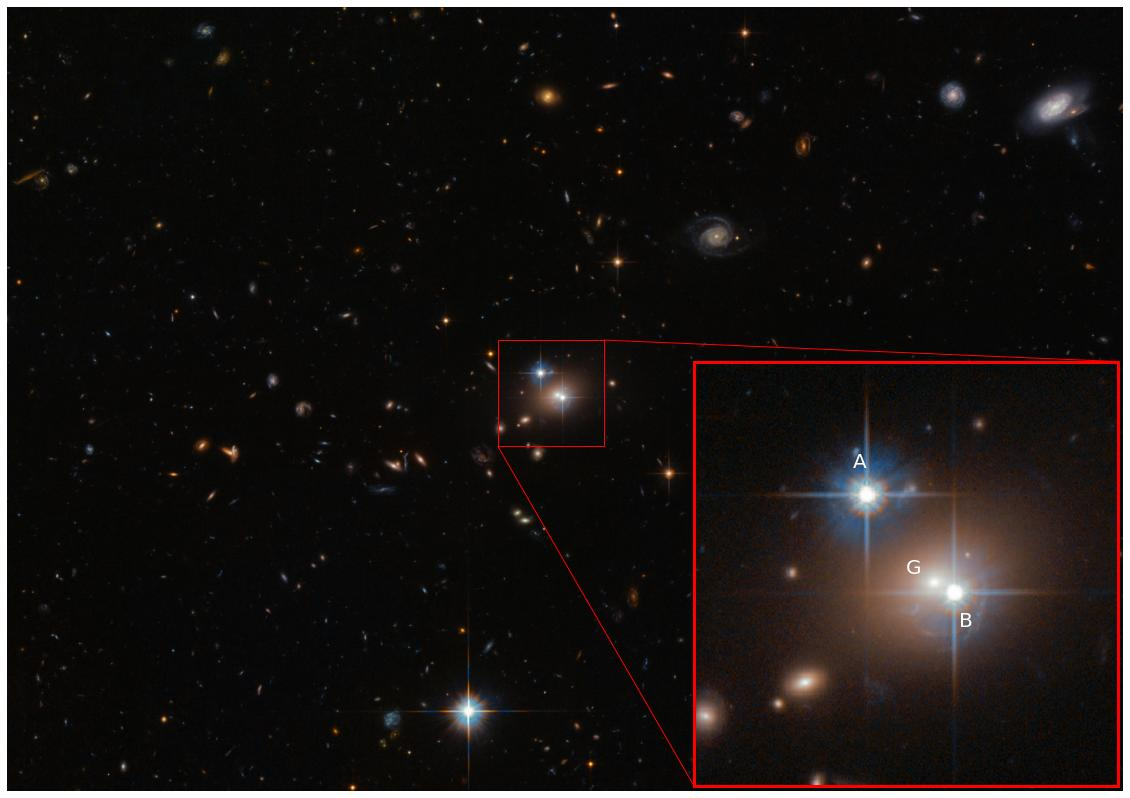
\includegraphics[width=0.8\textwidth]{figures/zoomed_in_qso0957}
        \caption{Le quasar double (QSO 0957+561 A et B) et la galaxie-lentille (G) imagée par le télescope spatial Hubble. 
        Crédit: ESA/Hubble et NASA, élargissement et annotation par AA.}
        \label{fig:doubel quasar}
\end{figure}

Dû à cette difficulté pratique, 
la première lentille gravitationnelle est découverte seulement plusieurs décennies après la prédiction de leur existence par \citet{Walsh1979}, 
suivant l'identification de deux spectres radios de quasars identiques, QSO 0957+561 A et B, séparés par $5.7$ secondes d'arcs
et capturés avec le télescope radio Mark II à l'observatoire Jodrell Bank. 
Les spectres partagent la même magnitude, $m=17$, le même décalage vers le rouge, $z=1.405$, et possèdent des détails 
chimiques suspicieusement semblables. Ces coïncidences suggèrent fortement que ces deux spectres sont des copies d'un seul objet, soit un noyau 
actif d'une galaxie en arrière-plan, produite par l'effet de lentille gravitationnelle d'une galaxie en avant-plan, invisible dans le 
domaine radio à une fréquence de $966\,\mathrm{MHz}$. Cette hypothèse est rapidement confirmée par 
l'observation optique de la galaxie-lentille ($z=0.355$) avec l'observatoire Palomar \citep{Young1980}\footnote{Simulténament 
observé et confirmé par le télescope de $2.2\, m$ de l'Université d'Hawaii au mont Mauna Kea \citep{Stockton1980}.}, 
ainsi que la modélisation de sa distribution de masse, de son environnement 
et des angles de déflexion qui causeraient l'apparition d'une image double du quasar \citep{Young1981,Falco1991}

À la suite de cette découverte fortuite, l'étude des lentilles gravitationnelles est devenue un sujet d'étude 
particulièrement riche et prometteur en cosmologie \citep{Blandford1992,Bartelmann2010,Treu2010}. 
Par exemple, les lentilles gravitationnelles permettent de mesurer 
la constante de \citet{Hubble1929}, $H_0$, qui quantifie le taux de l'expansion de l'Univers au temps présent. Les deux méthodes principales 
pour faire cette mesure à l'aide des lentilles gravitationnelles sont la caractérisation de la courbe de lumière des supernovas lentillées 
\citep{Refsdal1964,Kelly2015,Goobar2017} 
et la surveillance décennale de quasars lentillés 
\citep[e.g.][]{Vanderriest1989,Wong2020}. 



\begin{figure}[tb!]
        \centering
        \begin{subfigure}[t]{0.45\textwidth}
                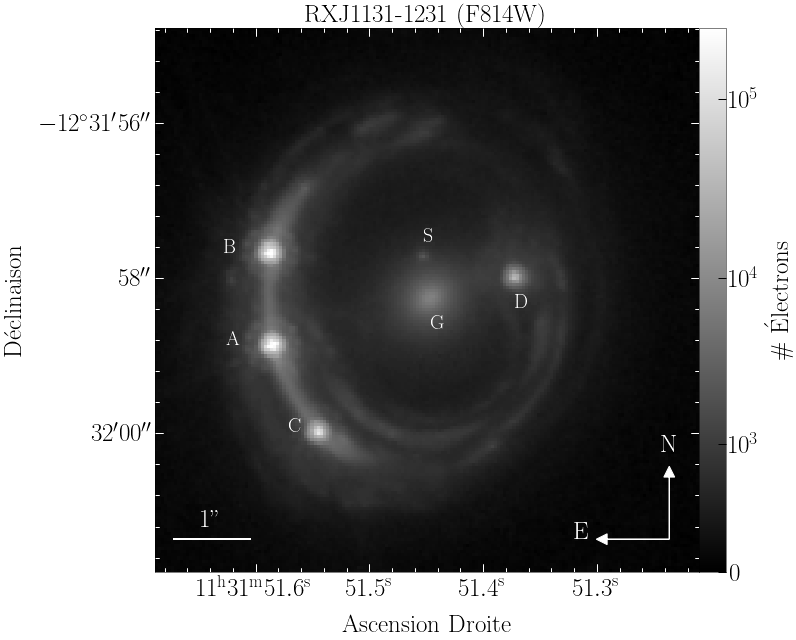
\includegraphics[width=\linewidth]{figures/rxj1131} 
                \caption{Quasar quadruplement lentillé (A, B, C et D) par une galaxie (G). L'image de la galaxie hébergeant le quasar 
                        est déformée tangentiellement, formant un anneau d'Einstein. Image prise par HST avec le filtre F814W.}
                \label{fig:rxj1131}
        \end{subfigure}
        ~
        \begin{subfigure}[t]{0.45\textwidth}
                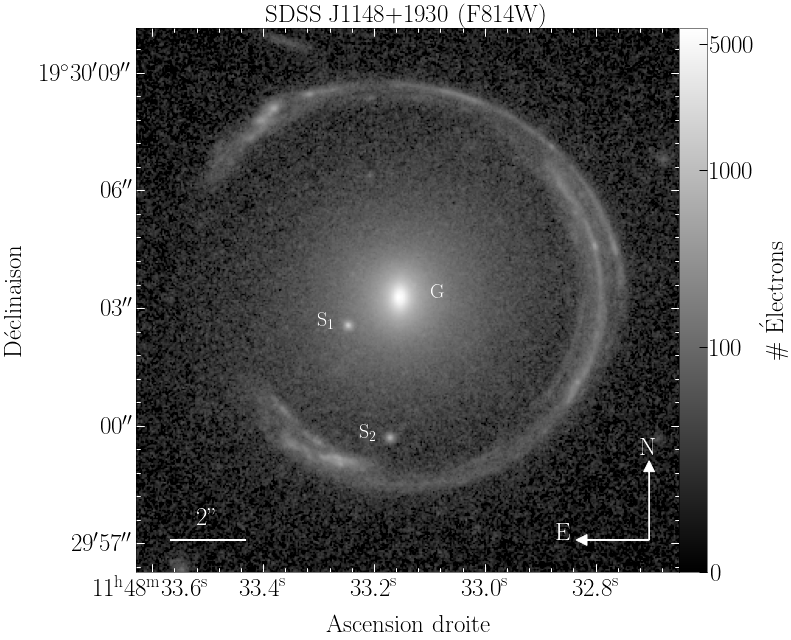
\includegraphics[width=\linewidth]{figures/sdssj1148} 
                \caption{Le fer à cheval cosmique, soit l'image d'une proto-galaxie à très haut décalage vers le rouge 
                        ($z=2.379$) fortement magnifiée et déformée par une galaxie elliptique lumineuse en infrarouge (G) exceptionnellement massive 
                        \citep[${5.2\times 10^{12}\, h_{72}^{-1}\, M_\odot}$,][]{Schuldt2019}. 
                 Image prise par HST avec le filtre F814W.}
                \label{fig:sdssj1148}
        \end{subfigure}
        \caption{Lentilles gravitationnelles de type galaxie-galaxie.}
        \label{fig:important lenses}
\end{figure}
 

De ce fait, plusieurs programmes ont été initiés pour trouver des lentilles gravitationnelles. Le programme 
\textit{Sloan Lens ACS Survey} \citep[SLAC,][]{Bolton2005,Bolton2006}, basé sur la recherche systématique de spectres de galaxies de type ETG\footnote{\textit{Early-Type Galaxies}} 
avec des lignes d'absorption à un décalage vers le rouge plus grand que les lignes d'émission, 
est un des programmes les plus réussis, ayant mené à la découverte 
confirmée de plus de $150$ lentilles gravitationnelles de type galaxie-galaxie \citep{Bolton2008,Shu2017}. Les programmes 
basés sur la recherche visuelle d'images doubles, triples, d'arcs ou d'anneaux \citep[e.g.][]{Faure2008} dans les 
champs du ciel larges et profonds comme 
COSMOS \citep{Koekemoer2007,Scoville2007}, connaissent aujourd'hui une renaissance nourrie par les succès récents de l'apprentissage profond 
pour la perception visuelle \citep{Krizhevsky2012}. Cette nouvelle approche a déjà mené à la découverte de plus de $1000$ lentilles 
gravitationnelles \citep{Petrillo2017,Huang2021}, et est projetée de découvrir plus de $10^{5}$ systèmes grâce 
aux nouveaux relevés du ciels prévus dans la prochaine décennie aux
observatoires Rubin \citep{lsst2009} et Euclid \citep{Euclid2010}.

%Le sujet du chapitre \ref{chap:censai} se concentre sur le défi de développer un algorithme pour modéliser la distribution de masse et 
%la morphologie de la source. Cet algorithme est dédié à analyser le nombre grandissant
%de lentilles gravitationnelles connues, dans toute leur complexité et dans un temps à l'échelle humaine. 
Dans la section qui suit, je dérive les équations centrales qui nous permettent 
d'étudier les lentilles gravitationnelles de type galaxie-galaxie.
Mon traitement est largement inspiré 
des manuels de références de \citet{Meneghetti2013,Congdon2018}. 


\section{Les angles de déflexion}

Supposons qu'un photon est sur une trajectoire parallèle à l'axe de 
visée $\mathbf{e}_{\parallel}$ d'un observateur sur Terre. 
Supposons de plus que la source d'un champ gravitationnel $\Phi$ est située sur l'axe de visée, 
ce qui a pour effet de courber la 
trajectoire de ce photon entre son point d'origine et son point d'arrivée.
On définit l'angle de déviation comme la déviation totale de cette trajectoire 
dans la direction perpendiculaire à l'axe de visée de l'observateur. 
De façon générale, cette déviation s'écrit
\begin{equation}\label{eq:intro alpha}
        \boldsymbol{ \alpha} = - \int_{\lambda_A}^{\lambda_B} \ddot{\mathbf{x}} \times \mathbf{e}_{\parallel} d\lambda\, ,
\end{equation}
où $\lambda$ paramétrise la trajectoire du photon $\mathbf{x}(\lambda)$. 
Le signe négatif nous indique qu'on prend la perspective de l'observateur. 

La trajectoire d'un photon obéit au 
principe de Fermat, qui stipule que la lumière suit une trajectoire qui extrémise
la durée du parcours entre deux points. 
Dans le langage du calcul 
des variations, la variation de la durée s'écrit
\begin{equation}\label{eq:Fermat}
        \delta T =  \delta \int_{A}^{B} n(\mathbf{x}(\ell)) \frac{d\ell}{c}= 0\, ,
\end{equation}
où $\ell$ est un élément de longueur sur la trajectoire et $n$ est un indice de réfraction.
Pour déterminer l'indice de réfraction du champ gravitationnel d'une galaxie, 
on doit utiliser le formalisme de la relativité générale. Selon le principe 
d'équivalence (fort), 
l'effet d'un champ gravitationnel est localement 
indistinguable d'une accélération causée par la courbure 
d'un espace-temps décrit par 
une métrique $g_{\mu \nu}$. 
La trajectoire d'un photon se trouve alors en cherchant 
les géodésiques de cet espace-temps. 
On fait l'approximation 
que le potentiel $\Phi$ d'une galaxie est celui d'un gaz parfait, c'est-à-dire 
qu'il satisfait une équation de Poisson
\begin{equation}\label{eq:Poisson}
       \grad^{2}\Phi = 4\pi G \rho .
\end{equation} 
Dans la limite où ce potentiel est faible $\displaystyle \frac{2\Phi}{c^{2}} \ll 1$, la 
métrique $g_{\mu \nu}$ est décrite par une expansion au premier ordre autour de la 
métrique de Minkowsky %$\eta_{\mu\nu}$
\begin{equation}\label{eq:metrique}
        ds^2 = g_{\mu\nu}dx^{\mu}dx^{\nu} \approx \left( 1 + \frac{2\Phi}{c^{2}} \right)c^{2}dt^{2} - \left( 1 - \frac{2\Phi}{c^{2}} \right)d\mathbf{x}^{2}.
\end{equation} 
Puisqu'un photon suit une géodésique de l'espace-temps $ds^{2} = 0$, on peut déterminer 
l'indice de réfraction en réarrangeant l'équation \eqref{eq:metrique}
\begin{equation}\label{eq:n}
        n \equiv c \left( \frac{\lVert d \mathbf{x} \rVert}{dt}  \right)^{-1} \approx  1 - \frac{2\Phi}{c^{2}}.
\end{equation} 
En réécrivant l'élément de longueur $d\ell$ en termes du 
paramètre de la trajectoire
$
        d\ell = \left\lVert\frac{d  \mathbf{x} }{d\lambda} \right\rVert d\lambda,
$
on peut réécrire l'équation \eqref{eq:Fermat} sous la forme
\begin{equation}\label{eq:Fermat2}
        \delta \int_{\lambda_A}^{\lambda_B} n(\mathbf{x}) \lVert \mathbf{\dot{x}} \rVert d\lambda = 0.
\end{equation} 
Par correspondance avec la fonctionnelle de l'action 
$J(x) = \int_{\lambda_0}^{\lambda_1} \mathcal{L}(\lambda,\, x,\,\dot{x}) d\lambda$, on trouve que 
le lagrangien de la trajectoire s'écrit 
$
        \mathcal{L} = n(\mathbf{x})  \sqrt{\dot{x}^{2}}.
$
La trajectoire qui satisfait \eqref{eq:Fermat} 
est une solution des équations d'Euler-Lagrange
\begin{equation}\label{eq:EulerLagrange}
        \frac{d }{d \lambda} \frac{\partial \mathcal{L}}{\partial \dot{\mathbf{x}}} - \frac{\partial \mathcal{L}}{\partial \mathbf{x}} = 0.
\end{equation} 
On a donc
\begin{equation}\label{eq:EulerLagrange2}
        \frac{d }{d \lambda} n \frac{\dot{\mathbf{x}}}{\lVert \dot{\mathbf{x}} \rVert}- \lVert \dot{\mathbf{x}} \rVert \grad n = 0 ,
\end{equation} 
Puisque le choix du paramètre $\lambda$ est libre, on peut le choisir tel 
que $\lVert \dot{\mathbf{x}} \rVert = 1$ en tout point de la trajectoire. Ainsi,
\begin{align}
        \nonumber
        \frac{d }{d \lambda} n \dot{\mathbf{x}} -  \grad n &= 0 \\
\label{eq:EulerLagrange3}
        \implies n \ddot{\mathbf{x}} + (\grad n \cdot \dot{\mathbf{x}}) \dot{\mathbf{x}} - \grad n &= 0
\end{align} 

À ce point de la dérivation, on utilise l'approximation de Born. 
C'est-à-dire qu'on approxime la trajectoire 
du photon comme une ligne droite sur l'axe de visée $\mathbf{e}_{\parallel}$. 
Cette approximation est justifiée 
dans le contexte des lentilles gravitationnelles de type galaxie-galaxie, 
puisque les angles de déviation sont généralement de 
l'ordre de l'arcseconde ou plus petits. 
Comme le vecteur $\dot{\mathbf{x}}$ est tangent à la trajectoire du photon, les termes $ \propto \dot{\mathbf{x}} \times \mathbf{e}_{\parallel} $ s'annulent. 
En subsitutuant l'indice de réfraction par \eqref{eq:n} dans $\mathbf{e}_{\parallel} \times \eqref{eq:EulerLagrange3}$, on obtient
\begin{equation}\label{eq:sol}
        \ddot{\mathbf{x}} \times \mathbf{e}_{\parallel} = \frac{1}{n} \grad_\perp n = \grad_\perp \log n
        \approx -\frac{2}{c^{2}}\grad_{\perp} \Phi\,,
\end{equation} 
où $\grad_\perp$ est un gradient selon les coordonnées perpendiculaires à $\mathbf{e}_\parallel$.
On note que le facteur 2 qui apparaît dans l'équation \eqref{eq:sol} est un 
effet qui vient de la relativité générale. Ce facteur corrige la solution 
que l'on aurait obtenue avec une dérivation classique (newtonienne).


On est maintenant en mesure de calculer l'angle de déviation. 
J'introduis le paramètre d'impact $\boldsymbol{\xi}$ qui est la distance perpendiculaire entre 
la position d'origine du photon sur le plan de la lentille  
et l'axe de visée (voir Figure \ref{fig:cartoon}).
Dans le cas où le potentiel est généré par une masse $M$ ponctuelle, c.-à-d.\ qu'on 
suppose $\rho = M\delta^{3}(\mathbf{x})$, où $\delta $ est la fonction delta de Dirac, 
alors le potentiel qui satisfait l'équation de Poisson \eqref{eq:Poisson} est 
la fonction de Green 
$\displaystyle \Phi = -\frac{GM}{\sqrt{ \xi^{2} + z^{2}}}$, où $z$ est la coordonnée 
sur l'axe de visée. L'équation \eqref{eq:intro alpha} se réécrit finalement comme 
\begin{align}
\nonumber
        \boldsymbol{ \alpha}(\boldsymbol{ \xi} ) &= -\frac{2GM}{c^{2}} \int_{-\infty }^{\infty }  \frac{\partial}{\partial \boldsymbol{\xi} }\frac{1}{(\xi^{2} + z^{2})^{1/2}}dz \\
\label{eq:deflection approx}
        \implies \boldsymbol{ \alpha}(\boldsymbol{ \xi})  &= \frac{4GM}{c^{2}  \xi^{2} } \boldsymbol{ \xi}
\end{align} 
Cette solution se généralise naturellement à un profil de masse quelconque en assumant 
qu'il s'exprime comme une somme d'éléments de masse $dm = \Sigma d^{2}\boldsymbol{ \xi}'$, 
où $\Sigma = \int \rho dz$ est une densité surfacique de masse. 
L'angle de déviation total mesuré à un point $\boldsymbol{\xi} $ est alors une convolution 
sur tout le plan de la lentille (mince) puisque l'équation \eqref{eq:deflection approx} dépend 
linéairement de la masse $M$:
\begin{equation}\label{eq:alpha physique}
        \boldsymbol{ \alpha} (\boldsymbol{ \xi} ) = \frac{4 G}{c^{2}} 
        \int_{\mathbb{R}^{2}} \Sigma (\boldsymbol{ \xi} ')
        \frac{\boldsymbol{ \xi}  - \boldsymbol{ \xi} '}{\lVert \boldsymbol{ \xi}  - \boldsymbol{ \xi} ' \rVert^{2}}d^{2}\boldsymbol{ \xi} '
\end{equation} 

\begin{figure}[tb!]
        \centering
        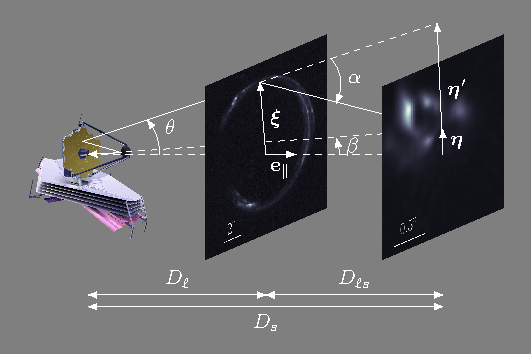
\includegraphics[width=0.8\textwidth]{figures/lensing_cartoon}
        \caption{Schéma d'une lentille gravitationnelle.}
        \label{fig:cartoon}
\end{figure}

L'angle de déviation est une quantité cruciale pour résoudre une lentille gravitationnelle 
puisqu'il décrit une transformation des coordonnées angulaires du plan de la lentille ($\boldsymbol{ \theta} $) 
vers les coordonnées angulaires du plan de la source ($\boldsymbol{ \beta} $). 
On assume que les distances entre l'observateur et la lentille $D_{\ell}$, entre l'observateur et la source $D_s$ et entre la lentille et la source $D_{\ell s}$, 
sont beaucoup plus grandes que les distances perpendiculaires à l'axe de visée $\boldsymbol{ \xi} $ ou $\boldsymbol{ \eta}$ 
(voir figure \ref{fig:cartoon}). 
Cette approximation est justifiée pour les objets qui nous intéressent,
pour lesquels les distances parallèles à l'axe de visée sont généralement 
de l'ordre du Gpc, alors que les distances perpendiculaires sont généralement 
de l'ordre du kpc; soit 6 ordres de grandeur de différence.
Ainsi, on peut faire un argument géométrique (euclidien) 
\begin{align}
\nonumber
       D_{s} \boldsymbol{ \theta} &= \boldsymbol{ \eta}' \\   
\nonumber
       D_{s} \boldsymbol{ \beta} &= \boldsymbol{ \eta} \\   
\nonumber
       D_{\ell s} \boldsymbol{ \alpha} &= \boldsymbol{ \eta}' - \boldsymbol{ \eta}  \\   
\label{eq:lens equation}
       \implies D_s \boldsymbol{ \beta} &= D_s \boldsymbol{ \theta} - D_{\ell s} \boldsymbol{ \alpha}   
\end{align} 
La dernière relation est l'équation maîtresse qui nous permet de tracer les rayons lumineux d'une source 
vers un détecteur fictif dans nos simulations. 

On notera que cette relation reste valide pour un Univers courbe et/ou en expansion 
(c.-à-d.\ décrit par une géométrie non euclidienne), 
à condition qu'on utilise une notion de distance qui satisfait, par définition, la relation trigonométrique euclidienne
\begin{equation}\label{eq:diameter angular distance}
       D \equiv \frac{\xi}{\theta}\, ,
\end{equation} 
où $\xi$ est la taille physique d'un objet placé à une certaine distance de l'observateur, et $\theta$ est l'angle solide sous-tendu 
par cet objet. Pour un Univers décrit par la métrique de Friedmann-Lemaître-Robertson-Walker,
la notion de distance qui respecte la définition \eqref{eq:diameter angular distance} est la distance du diamètre angulaire. 
En pratique, on peut exprimer $D$ en termes du décalage vers le rouge des photons émis par l'objet, $z$. 
On note $a(z)$ le facteur d'échelle lorsque le photon est émis par la source et $a(0)$ le facteur d'échelle au moment présent ($z=0$).
Pour un Univers plat \citep[voir les manuels de référence][]{Coles2002,Dodelson2003,Bartelmann2004}
\begin{align}
        D_z &= c a(z) \underbrace{\int_{a(z)}^{a(0)} \frac{da}{a \dot{a}}}_{\strut\mathclap{\text{distance comobile}}}; \\[2ex]
                \nonumber
              &= \frac{c a(z)}{H_0} \int_{a(z)}^{a(0)} \frac{da}{\sqrt{\Omega_{r,0} + \Omega_{m,0} a  + \Omega_{\Lambda,0}a^{4}}}; \\
              \label{eq:dang}
              &= \frac{c}{H_0(1 + z)} \int_{0}^{z} \frac{dz'}{\sqrt{\Omega_{r,0}(1 + z')^{4} + \Omega_{m,0} (1 + z')^{3} + \Omega_{\Lambda,0} }}\, .
\end{align}
On a utilisé la relation entre le facteur d'échelle, $a$, et le décalage vers le rouge, $a = (1 + z)^{-1}$, pour obtenir l'équation \eqref{eq:dang} 
par un changement de la variable d'intégration. 
$\Omega_{r,0}$, $\Omega_{m,0}$ et $\Omega_{\Lambda, 0}$ sont les paramètres de densités, au temps présent, de la radiation, de la matière et de l'énergie sombre 
respectivement. 
%$\Omega_K = 1 - \Omega_0$ est le paramètre de courbure et 
$H_0$ est la constante de Hubble, soit le taux 
d'expansion de l'Univers au temps présent. La distance $D_{\ell s}$ se trouve simplement en ajustant les bornes de l'intégrale $\int_0^{z} \mapsto \int_{z_\ell}^{z_s}$.
La valeur des paramètres du modèle cosmologique $\Lambda$CDM obtenue par l'équipe \citet{PlanckCollaboration2018}
est rapportée dans l'annexe \ref{app:lcdm}.


Il est généralement pratique de travailler avec la forme adimensionnelle de l'équation \eqref{eq:lens equation}. 
On introduit la densité critique 
\begin{equation}\label{eq:densite critique}
        \Sigma_c = \frac{c^2}{4 \pi G}\frac{D_{s}}{D_{\ell s} D_\ell}\, ,
\end{equation} 
qui nous permet de définir la quantité qu'on nomme convergence $\displaystyle \kappa(\boldsymbol{ \theta} ) \equiv \frac{\Sigma(\boldsymbol{ \theta})}{\Sigma_c}$. 
On définit ainsi l'angle réduit 
\begin{equation}\label{eq:alpha adim}
        \hat{\boldsymbol{ \alpha}} (\boldsymbol{ \theta}) = \frac{1}{\pi}\int_{\mathbb{R}^{2}} \kappa(\boldsymbol{ \theta} )
        \frac{\boldsymbol{ \theta} - \boldsymbol{ \theta}'  }{\lVert \boldsymbol{ \theta} - \boldsymbol{ \theta}' \rVert  } d^{2}\boldsymbol{ \theta}'\, ,
\end{equation} 
qui satisfait l'équation de la lentille adimensionnelle 
\begin{equation}\label{eq:lens equation adim}
        \boldsymbol{ \beta} = \boldsymbol{ \theta} - \hat{\boldsymbol{ \alpha}}(\boldsymbol{ \theta})\, . 
\end{equation}

Les équations \eqref{eq:alpha adim} et \eqref{eq:lens equation adim} sont les équations centrales à 
la modélisation des lentilles gravitationnelles. Elles sont utilisées pour simuler des lentilles 
gravitationnelles au chapitre \ref{chap:censai}. Elles sont aussi utilisées pour résoudre le 
problème inverse qui consiste à inférer l'image non-distordu de la galaxie en arrière-plan, $I(\boldsymbol{ \beta})$, 
et les paramètres de la distribution de masse de la galaxie-lentille, $\kappa(\boldsymbol{ \theta})$,
à partir des distortions observées de l'image en arrière-plan $I(\boldsymbol{ \theta})$. 
%soit le problème inverse qui motive la recherche présentée dans ce mémoire.


  \chapter{Introduction à l'apprentissage profond}\label{chap:intro ml}

L'astronomie, l'astrophysique et la cosmologie sont officiellement entrées dans l'ère du \textit{Big Data}, 
soit une ère dominée par le volume de données, maintenant mesuré dans l'ordre du \textit{petabyte}. Un \textit{petabyte} représente 
un million de \textit{gigabytes}, ou encore $\sim 10^{15}$ \textit{bytes}. 
En exemple particulier est l'observatoire Vera C. Rubin. Cet observatoire produira environ 1 \textit{petabytes} de données chaque année, soit une quantité de données 
impossible à traiter dans son ensemble pour la plupart des algorithmes; 
sans parler de la quantité accumulée par l'observatoire au travers des 10 années planifiées pour le relevé astronomique qui doit débuter 
en $2024$ \citep{lsst2009,lsst2021}. 

C'est cette réalité qui nous force à développer des méthodes d'analyses plus sophistiquées pour l'inférence de quantités physiques à partir 
d'images, spectres et vidéos du ciel. C'est aussi ce qui motive l'étude des méthodes liées à l'apprentissage machine, et plus particulièrement 
l'apprentissage profond, qui promettent de simplifier énormément l'analyse statistique des grands ensembles de données à venir. Ce chapitre se veut 
une courte introduction aux concepts de base. 
La section \ref{sec:bayes} est un survol de la théorie des statistiques bayésiennes. Cette section introduit certains concepts cruciaux qui sous-tendent la 
théorie de l'apprentissage machine. Ensuite, la section \ref{sec:app classique} décrit en détail un exemple de régression, 
puis la section \ref{sec:selection modele} discute du problème de la sélection du modèle.
Les réseaux neuronaux et l'apprentissage profond sont introduits à la section \ref{sec:app profond} 
comme une généralisation possible de l'apprentissage machine classique. Finalement, on introduit les 
réseaux de neurones convolutifs à la section \ref{sec:cnn}, cruciaux pour le traitement d'images.

Pour une discussion plus détaillée des concepts abordés dans ce chapitre, voir les manuels de référence \citet{Goodfellow2016} et \citet{Bishop2007}.

\section{Survol des statistiques bayésiennes}\label{sec:bayes}

L'inférence bayésienne est une théorie statistique qui a pour but principal de modéliser l'état de connaissance, 
ou le degré de croyance, associé à un évènement. De façon générale, l'inférence bayésienne est un processus de mise à jour de nos 
connaissances \textit{a priori}, c.-à-d. les connaissances acquises avant l'observation d'un évènement. 
On définit la vraisemblance comme la loi de probabilité qui gouverne la probabilité d'observer un évènement particulier.
Étant donné un processus physique auquel on associe une loi de vraisemblance, le processus d'inférence 
bayésienne correspond simplement à la repondération de nos connaissances par la vraisemblance. 
En d'autres mots, cette procédure correspond à multiplier la loi de probabilité \textit{a priori} par la vraisemblance d'un évènement (et renormaliser).

Par exemple, considérons un tirage au sort. 
On modélise la probabilité, $x \in [0, 1]$, d'observer pile ou face, $y \in \{0, 1\}$, 
par une loi de Bernoulli 
\begin{equation}
        p(y \mid x) = x^{y} (1 - x)^{1 - y}\, .
\end{equation} 
\textit{A priori}, on associe une probabilité égale (uniforme) au paramètre $x$, soit $p(x) = \mathcal{U}(0, 1)$. 
Ce choix reflète une ignorance complète du processus physique qui contrôle le tirage au sort.
Supposons maintenant qu'on observe $y_1$, un évènement généré de la loi physique $p(y_1 \mid x^{\star})$, où $x^{\star}$ est le véritable paramètre de la loi physique.
Le théorème de Bayes nous indique comment ajuster notre degré de croyance, maintenant $p(x \mid y_1)$, soit la loi \textit{a posteriori} du paramètre $x$ étant donné avoir observé $y_1$
\begin{equation}\label{eq:Bayes1}
        p(x \mid y_1) = \frac{p(y_1 \mid x) p(x)}{p(y_1)} \, .
\end{equation} 
La loi de probabilité $p(y)$, aussi appelée l'évidence, normalise la loi \textit{a posteriori}, qui est proportionnelle au produit de la vraisemblance $p(y \mid x)$ et 
de la loi \textit{a priori} $p(x)$. En pratique, on peut évaluer $p(y)$, une loi marginale, en l'exprimant 
en fonction de la loi jointe $p(x, y)$, soit 
\begin{equation}
        p(y) = \int_\mathcal{X} dx\, p(y, x) \, .
\end{equation} 
On peut ensuite utiliser la définition d'une loi conditionnelle 
\begin{equation}
        p(y \mid x) = \frac{p(x,\, y)}{p(x)} \, ,
\end{equation} 
pour exprimer l'évidence, $p(y)$, en fonction de la vraisemblance et de la loi \textit{a priori} 
\begin{equation}
        p(y) = \int_\mathcal{X} dx\, p(y \mid x) p(x)\, .
\end{equation} 
Supposons maintenant qu'on observe un certain nombre de tirages au sorts supplémentaires
\begin{equation*}
        y_2,y_3\dots,y_N \overset{\mathrm{iid}}{\sim} p(y \mid x^{\star})\, ,
\end{equation*}
indépendamment et identiquement distribués (iid) selon la même loi physique, $p(y \mid x^{\star})$. Pour mettre à jour nos connaissances, on procède 
itérativement. En premier lieu, on trouve la distribution \textit{a posteriori} $p(x \mid y_1)$ avec le théorème de Bayes \eqref{eq:Bayes1}. Ensuite, 
on remplace la distribution \textit{a priori}, $p(x)$, par $p(x \mid y_1)$ et on remplace la loi de vraisemblance par $p(y_2 \mid x)$ dans le théorème de Bayes \eqref{eq:Bayes1} 
pour obtenir la loi \textit{a posteriori}, $p(x \mid y_1, y_2)$. Et ainsi de suite.
Puisque les observations sont iid, alors ce processus est équivalent, par induction, à 
\begin{equation}\label{eq:BayesN}
        p(x \mid y_{1:N}) = \frac{\prod_{i=1}^{N} p(y_i \mid x) p(x)}{\int_\mathcal{X} \prod_{i=1}^{N}p(y_{i} \mid x) p(x) dx}
\end{equation} 
Ce dernier résultat est particulièrement important pour l'inférence statistique et la dérivation des fonctions 
objectives pour l'apprentissage machine. La figure \ref{fig:bayes update} montre comment nos connaissances 
sur le paramètre $x$ évoluent en termes du nombre d'observations effectuées lorsqu'on applique l'équation \eqref{eq:BayesN}. 
La figure montre que la loi \textit{a posteriori} correspond à la loi \textit{a priori} lorsque $N = 0$ 
et converge vers une loi normale centrée autour de $x^{\star}=\frac{1}{2}$ lorsque $N \rightarrow \infty$, 
soit un exemple concret du théorème de la limite centrale.
\begin{figure}[H]
        \centering
        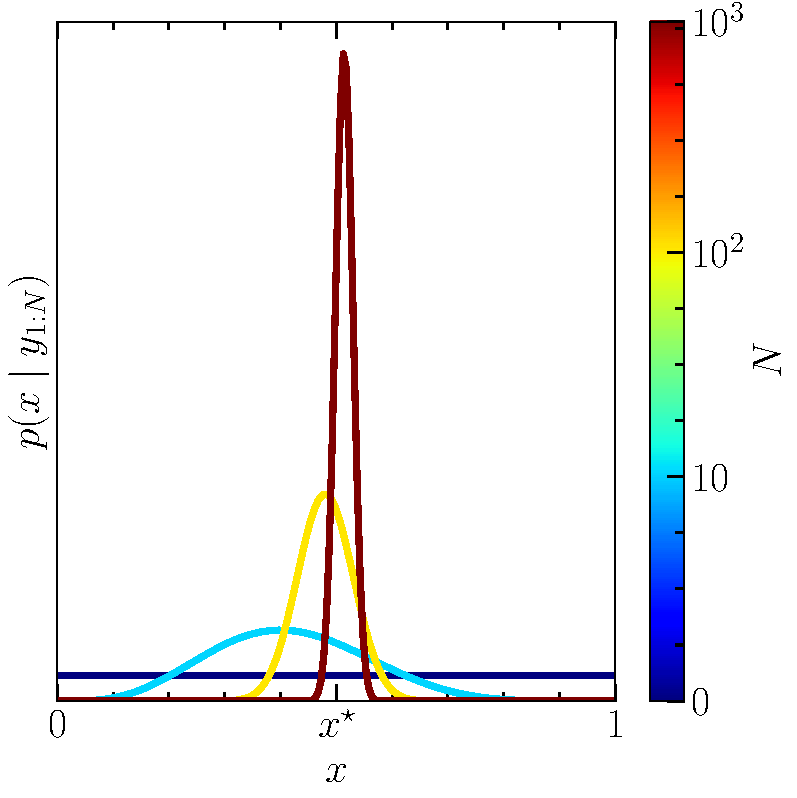
\includegraphics[width=0.4\textwidth]{notebooks/toy_coin_toss.pdf}
        \caption{Exemple d'une inférence bayésienne pour le tirage au sort.}
        \label{fig:bayes update}
\end{figure}

Le lecteur aura compris qu'on va maintenant construire l'apprentissage machine sur des fondations bayésiennes. Ce n'est pas la seule façon de le 
faire. En particulier, il est possible de poser des fondations fréquentistes en supposant, comme fait dans cette section, que toute l'information 
concernant un problème est contenue dans la loi de vraisemblance. Autrement dit, on suppose une ignorance complète \textit{a priori} sur les paramètres d'intérêts. 
En ce sens, et strictement dans le contexte qui nous intéresse, il est possible de passer d'un point de vue à l'autre, puisque les deux théories seront en accord 
sur la réponse à condition qu'on utilise une loi uniforme pour représenter nos connaissances \textit{a priori} sur les paramètres d'intérêts. 
À cause de cette correspondance approximative entre les deux théories, les lois 
\textit{a priori} vont parfois être abandonnées sans justification dans le texte qui suit. 
Le lecteur comprendra qu'on aura simplement changé de point de vue. 

\section{Un exemple d'apprentissage machine: la régression}\label{sec:app classique}

L'apprentissage machine est un concept assez général qui décrit le processus d'extraire l'information contenue 
dans un ensemble de données $\mathcal{D} = \{\mathbf{y}^{(i)}\}_{i=1}^{N}$, soit un ensemble d'observations provenant d'une source ou d'un processus 
physique quelconque. Le terme \textit{information} est utilisé de façon très vague ici. Ce terme est formellement défini dans la théorie 
de l'information de \citet{Shannon1948} comme étant le nombre minimal de \textit{bits} pour décrire une observation $y_i$, ou encore 
l'ensemble de données $\mathcal{D}$. Cette quantité est intimement liée avec l'entropie. Une discussion plus détaillée est 
repoussée au chapitre \ref{chap:intro ml 2}.

Il y a quatre ingrédients essentiels à l'apprentissage machine, soit
\begin{enumerate}
        \item Un ensemble de données $\mathcal{D}$
        \item Un ensemble d'hypothèses $\mathcal{H}$
        \item Une fonction objective $\mathcal{L}$
        \item Un algorithme d'optimisation $\mathcal{G}$
\end{enumerate}
Dans cette section, je décris chacun de ces ingrédients dans le contexte d'une tâche de régression.
La régression est une tâche d'apprentissage machine qui consiste à entraîner un modèle, $f_{\theta}$, sur un ensemble de données augmenté pour la régression, soit 
$\mathcal{D} = \{(\mathbf{x}^{(i)}, \mathbf{y}^{(i)})\}_{i=1}^N$. 
Chaque exemple dans l'ensemble de données est constitué d'un vecteur de paramètres physiques, $\mathbf{x}$, et d'une observation, $\mathbf{y}$. 
On suppose toujours que les exemples de l'ensemble de données sont générés de façon identique et indépendante par la combinaison 
d'une loi \textit{a priori} sur les paramètres physiques et une loi de vraisemblance pour les observations
\begin{equation}
                \mathbf{x} \sim p(\mathbf{x}),  \hspace{1cm} \mathbf{y}\ \sim p_\theta(\mathbf{y} \mid \mathbf{x}) \, . 
\end{equation}
Dans le texte, on utilisera le terme \textit{modèle physique} pour faire référence à $p_\theta(\mathbf{y} \mid \mathbf{x})$, puisque cette loi de probabilité relie les paramètres physiques
avec les observations. Elle encodera donc tous les processus physiques en jeu pour un problème d'inférence donné.
On notera de plus que l'ensemble des points de données n'a pas besoin d'être un nombre fini. Dans le cas où $N \rightarrow  \infty$, alors 
$\mathcal{D}$ est explicitement décrit par la loi \textit{a priori}, $p(\mathbf{x})$, et le modèle physique $p_\theta(\mathbf{y} \mid \mathbf{x})$. 
Dans ce cas, on dira que la loi générative $(\mathbf{x}, \mathbf{y}) \sim p(\mathbf{x}, \mathbf{y})$ est explicite. 
Dans le cas où $\mathcal{D}$ est un nuage de points ($N < \infty$), alors on dira que le processus génératif est implicite. 

Pour se fixer les idées, on considère l'exemple  
\begin{equation}\label{eq:loi generative}
        p(x) = \mathcal{U}(a, b), \hspace{1cm} p_\theta(y \mid x) = \mathcal{N}(y \mid f_\theta(x), \sigma^2)\, .
\end{equation}
On a utilisé le symbole $\mathcal{N}(y \mid \mu, \sigma^2)$ pour décrire une loi normale sur $y$ avec comme moyenne $\mu$ et variance $\sigma^2$. 
On doit supposer que les données sont générées à partir d'une solution quelconque 
\begin{equation}
        f_{\theta^{\star}} = 2x^5 - x\, ,
\end{equation}
avec une amplitude de bruit $\sigma=1$. Ce problème est illustré à la figure \ref{fig:toy problem}.
\begin{figure}[th!]
        \centering
        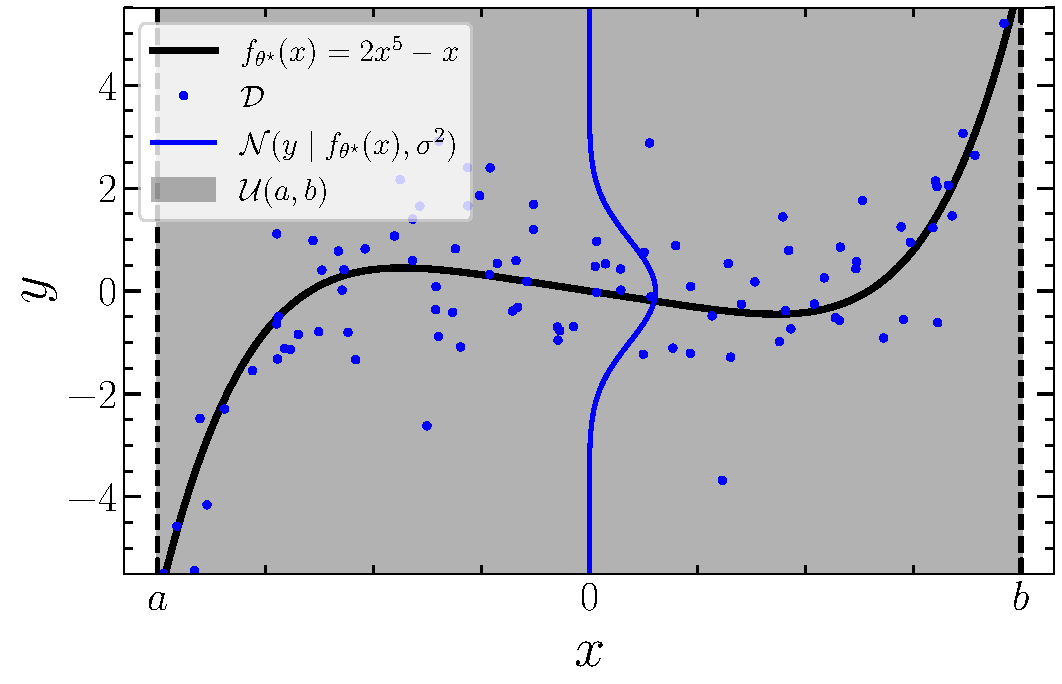
\includegraphics[width=0.5\textwidth]{notebooks/toy_problem}
        \caption{Exemple d'un problème de régression.}
        \label{fig:toy problem}
\end{figure}

Le second ingrédient au problème d'apprentissage machine est la famille des modèles, ou l'ensemble des hypothèses, $\mathcal{H}$. 
Il serait tentant de choisir le modèle $f_\theta = \theta_1 x^{5} + \theta_2 x$, soit un modèle avec la même forme que la solution 
$f_{\theta^{\star}}$. Toutefois, on ne peut pas supposer que la forme du modèle sera connue \textit{a priori}, 
ou qu'elle peut facilement être devinée. La sélection du modèle sera abordée en détail dans la section \ref{sec:selection modele}, 
puisque ce sujet mérite une discussion à part entière.
Pour l'instant, on va simplement faire le choix le plus simple en assumant que la forme de 
la loi utilisée pour générer les points de données est inconnue. 
Le choix le plus simple est de construire une famille de modèles linéaires en termes de $x$ et $\theta$
\begin{equation}\label{eq:modele lineaire}
        \mathcal{H} = \{f_\theta:\mathbb{R} \rightarrow  \mathbb{R} \mid f_\theta = \theta_0 + \theta_1 x\}\, . 
\end{equation} 
Le troisième ingrédient à l'apprentissage machine est de construire une fonction objective pour \textit{entrainer} notre modèle $f_\theta$ sur les points 
de données observés. 
L'objectif de l'entraînement est d'estimer le modèle $f_\theta$, ou de façon équivalente les paramètres $\theta$, qui maximise la loi \textit{a posteriori}, $p(\theta | \mathcal{D})$. En appliquant 
le théorème de Bayes, ceci correspond à
\begin{equation}
        \hat{\theta} = \underset{f_\theta \in \mathcal{H}_\theta}{\mathrm{arg\, max}}\, \frac{p(\mathcal{D} \mid \theta) p(\theta)}{p(\mathcal{D})}
\end{equation} 
Pour faire correspondre cet objectif avec la littérature, on applique le logarithme au côté droit de l'équation, ce qui ne change pas la position des extremas de 
l'objectif, le logarithme étant une fonction monotone. Il est aussi convention de tourner le problème à l'envers, et de chercher plutôt les minimas de la fonction négative. Dans 
ce cas, la fonction objective est
\begin{equation}
        \hat{\theta} = \underset{f_\theta \in \mathcal{H}}{\mathrm{arg\, min}}\, -\log p(\mathcal{D} \mid \theta) - \log p(\theta) + C(\mathcal{D})\, .
\end{equation} 
où $C(\mathcal{D})$ est une constante qui ne dépend que de l'ensemble de données. L'étape finale est d'écrire la vraisemblance $p(\mathcal{D} \mid \theta)$ 
en termes de $p_\theta( y \mid x)$. Dans le texte, les paramètres d'entraînements sont toujours placés en indices, 
par quoi on entend que les paramètres $\theta$ conditionnent la loi de probabilité, $p_\theta(x \mid y) = p(x \mid y, \theta)$. On remarque que
\begin{equation}
        p(\mathcal{D} \mid \theta) = \prod_{i=1}^{N}p(x_i, y_i \mid \theta) = \prod_{i=1}^{N}p(y_i \mid x_i, \theta) p(x_i \mid \theta)\, ,
\end{equation} 
par définition de la loi conditionnelle et de la supposition que les données sont générées de façon iid. 
Le dernier terme peut être simplifié en termes de la loi \textit{a priori}, $p(x \mid \theta) = p(x)$ 
puisqu'on suppose que $\theta$ et $x$ sont deux variables aléatoires indépendantes. Un choix de modèle $\theta$ ne devrait pas changer 
la distribution \textit{a priori} sur les paramètres physiques. Si c'est le cas, alors le choix du modèle doit être révisé.
On trouve finalement l'objectif d'entraîenement
\begin{equation}
        \hat{\theta} = \underset{f_\theta \in \mathcal{H}}{\mathrm{arg\, min}}\, -\log \prod_{i=1}^{N}p_\theta(y_i \mid x_i) - \log p(\theta) + C(\mathcal{D})\, ,
\end{equation} 
où $-\log \prod_{i=1}^N p(x_i)$ est absorbé dans $C(\mathcal{D})$. On est maintenant en mesure de dériver la forme exacte de la fonction objective pour le problème 
posé dans cette section. Avec la supposition que le modèle physique est une loi normale, on a que
\begin{equation}
       \log \prod_{i=1}^{N}p_\theta(y_i \mid x_i) = -\frac{1}{2}\sum_{i=1}^{N}\frac{(y_i - f_\theta(x_i))^2}{\sigma^2} - \frac{N}{2}\log(2\pi \sigma^2)\, ,
\end{equation} 
ce qui correspond à la fonction objective
\begin{equation}\label{eq:MSE intro}
        \hat{\theta} = \underset{f_\theta \in \mathcal{H}}{\mathrm{arg\, min}}\, \underbrace{ \frac{1}{N}\sum_{i=1}^{N}
        (y - f_\theta(x))^2 }_{\hat{\mathcal{L}}_\theta(\mathcal{D})}  - \frac{2\sigma^2}{N}\log p(\theta)\, .
\end{equation} 
Par convention, on a utilisé le fait que les constantes qui ne dépendent pas de $\theta$ peuvent être ignorées (elles ne changent pas les extremas du problème) 
et on a multiplié la fonction objective par $2\sigma^2 / N$. 
L'expression obtenue fait intervenir la fonction objective approximative $\hat{\mathcal{L}}_{\theta}(\mathcal{D})$, soit un estimé Monte Carlo de l'espérance de l'erreur 
quadratique. En prenant la limite $N \rightarrow \infty$, l'estimé Monte Carlo de l'espérance devient exacte
\begin{equation}
        \lim\limits_{N \rightarrow \infty}\hat{\mathcal{L}}(\mathcal{D}) = \mathcal{L}_{\theta}(\mathcal{D}) = \mathbb{E}_{(x, y) \sim \mathcal{D}} \big[(y - f_\theta(x))^2\big]\, .
\end{equation} 
Dans la littérature, $\hat{\mathcal{L}}_\theta(\mathcal{D})$ est nommée l'erreur quadratique moyenne. Dans le reste de ce mémoire, on va laisser 
tomber le chapeau sur la fonction objective pour simplifier la notation. Le lecteur comprendra qu'on travaille généralement avec l'estimé 
Monte Carlo si l'espérance mathématique n'est pas accessible par calcul direct.

Le dernier ingrédient à l'apprentissage machine est le choix d'un algorithme d'optimisation $\mathcal{G}$ pour résoudre l'équation \eqref{eq:MSE intro}, c.-à-d. déterminer 
$\hat{\theta}$. Les algorithmes d'optimisations récents pour l'apprentissage profond sont souvent basés sur la descente de gradient stochastique, qu'on peut décrire succinctement 
par la relation de récurrence
\begin{equation}\label{eq:gd}
        \hat{\theta}^{(t+1)} = \hat{\theta}^{(t)} - \gamma_t \grad_{\hat{\theta}^{(t)}} \mathcal{L}_{\hat{\theta}^{(t)}}(\mathcal{D})\, ,
\end{equation} 
$\gamma_t$ est le taux d'apprentissage, généralement choisi comme étant aussi grand que possible, 
sans pour autant rendre instable l'algorithme d'optimisation $\mathcal{G}$. Une discussion plus détaillée est reportée au chapitre \ref{chap:intro ml 2} sur ce sujet.

\begin{figure}[th!]
        \centering
        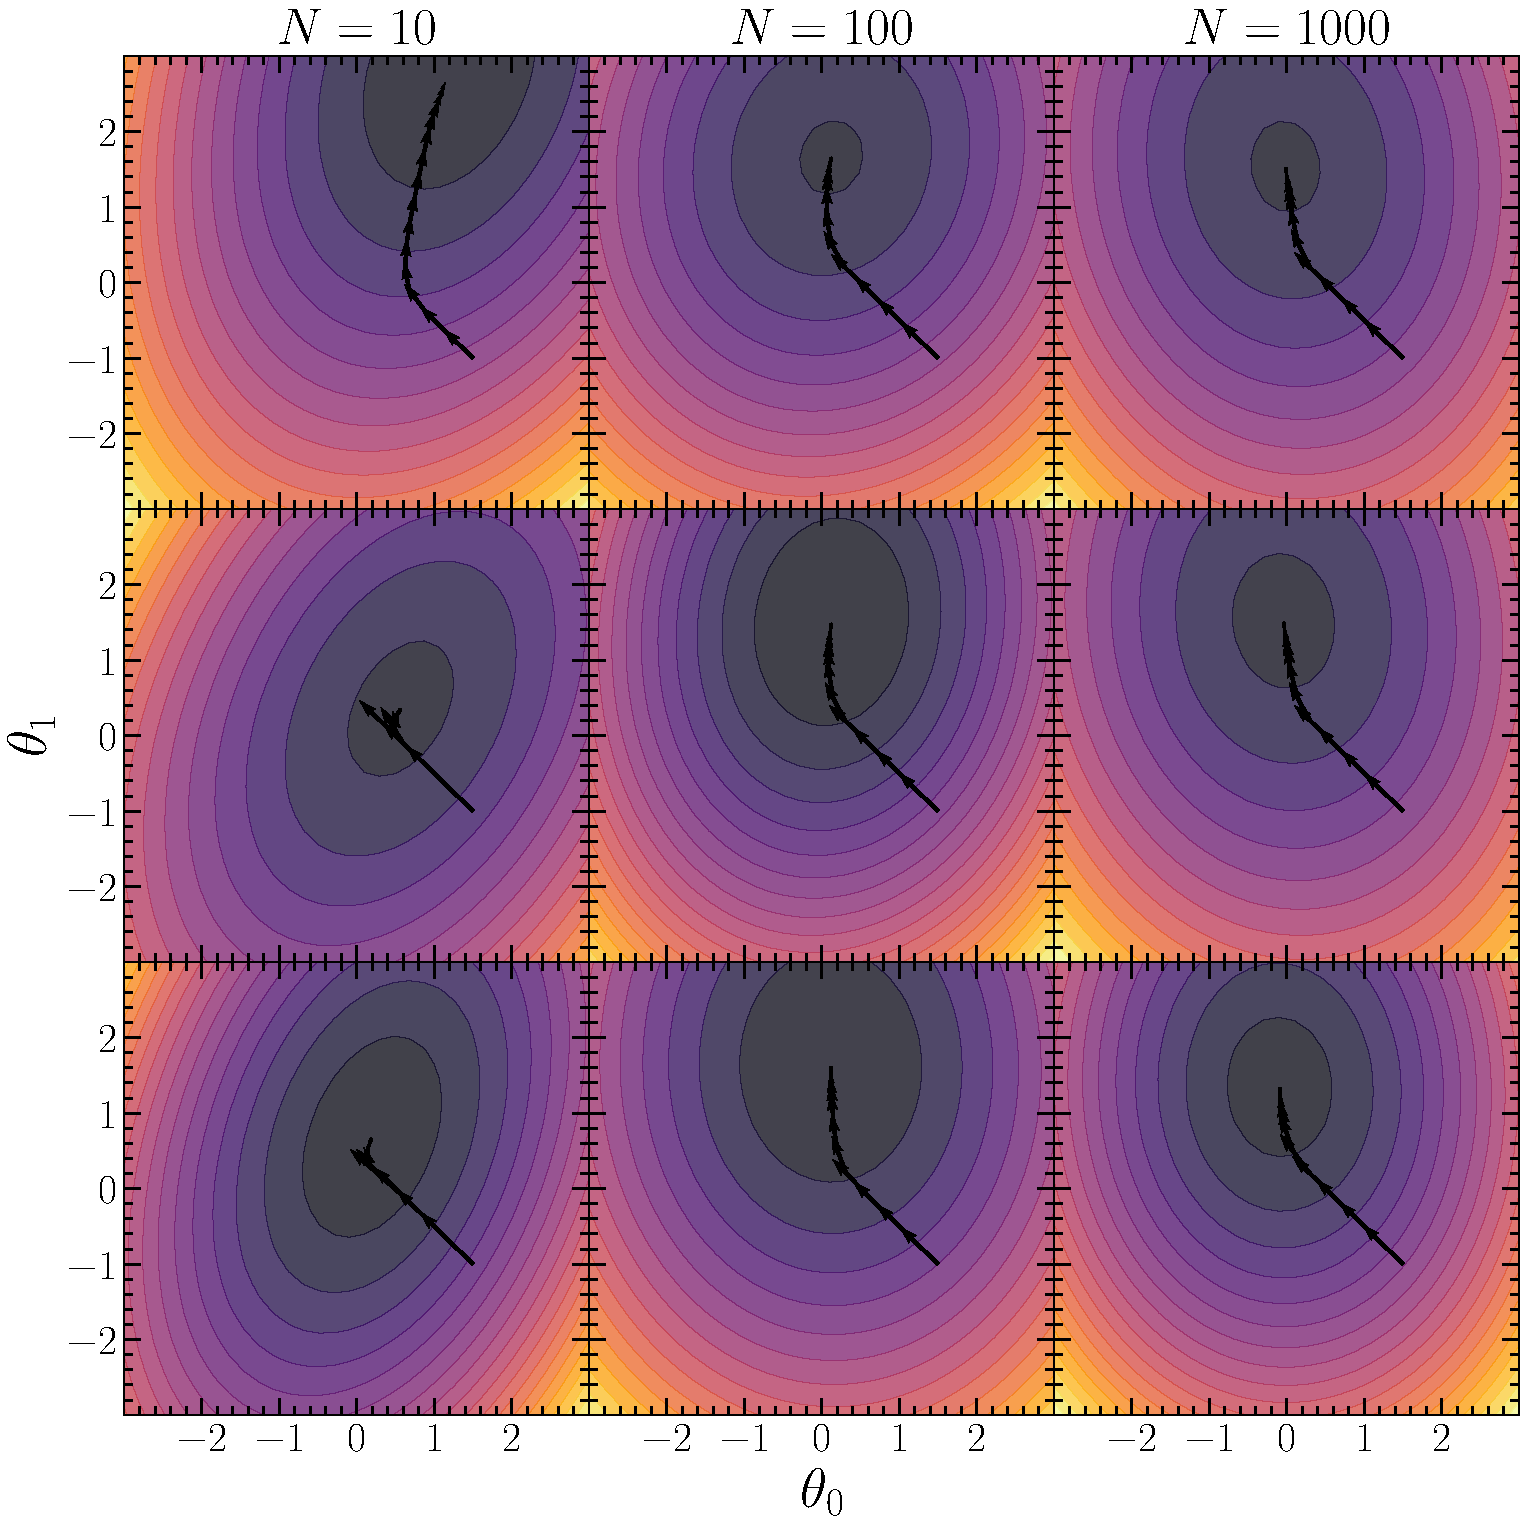
\includegraphics[width=0.7\textwidth]{notebooks/monte_carlo_loss.pdf}
        \caption{Contours de $\mathcal{L}_\theta(\mathcal{D})$ pour différent tirage de $\mathcal{D}$ (rangées) et différentes taille $N = |\mathcal{D}|$ (colonnes) 
                en utilisant le modèle linéaire de l'équation \eqref{eq:modele lineaire} et la loi générative \eqref{eq:loi generative}.
        Une trajectoire produite par la descente de gradient \eqref{eq:gd} est illustré avec les flèches noires.}
        \label{fig:monte carlo L}
\end{figure}

Lorsqu'on travaille à basses dimensions, il est possible d'obtenir de très bons estimés pour $\mathcal{L}_\theta(\mathcal{D})$. 
Par exemple, la figure \ref{fig:monte carlo L} illustre comment 
la variance des contours de l'estimé Monte Carlo $\mathcal{L}_{\theta}(\mathcal{D})$ diminue en fonction de $N$. 
Les rangées montrent un estimé Monte Carlo pour différents tirages de l'ensemble de données $\mathcal{D}$ à partir 
de la loi générative décrite à l'équation \eqref{eq:loi generative}, alors que les colonnes montrent  
des ensembles de données de taille croissante. En particulier, la troisième colonne possède des contours très stables, ce qui 
implique que la descente de gradient va retrouver la même solution $\hat{\theta}$ systématiquement, 
contrairement aux estimés où $N$ est relativement petit. Dans ce cas, la solution obtenue par $\mathcal{G}$ 
dépend fortement de l'ensemble de données observé; la première colonne est l'exemple le plus frappant de ce phénomène.


%Je termine cette courte introduction avec la définition de deux concepts qui portent parfois à confusion 
%dans le jargon de l'apprentissage profond, soit celui d'une \textit{batch} et d'une \textit{époque}.  
%Une \textit{batch} $\mathcal{B}$ est un sous ensemble de $\mathcal{D}$, soit $\mathcal{B} \subseteq \mathcal{D}$. Dans le même ordre d'idée du paragraphe précédent, les fonctions objectives 
%estimées à partir de différentes \textit{batch}, $\mathcal{L}(\mathcal{B})$, peuvent varier de manière significative entre chaque \textit{batch}. 
%Toutefois, sous certains conditions, une descente stochastique avec \textit{batch} est équivalente à une descente de gradient stoachastique avec $\mathcal{L}(\mathcal{D})$, 
%soit un estimé à partir de l'ensemble de donnée complet. La descente de gradient stochastique avec \textit{batch} 
%est donc particulièrement utile pour l'optimisation de modèles où les données traitées sont de très haute dimensions, 
%une situation où l'obtention de la quantité $\mathcal{L}(\mathcal{D})$ requiert souvent une quantité d'opérations machines prohibitive, contrairement à $\mathcal{L}(\mathcal{B})$.
%D'un autre côté, une \textit{époque} est un concept assez artificiel qui n'est pas réutilisé dans le reste de ce mémoire. Ce concept correspond à un 
%certains nombre d'itérations de la descente de gradient après lequel on aurait épuisé l'ensemble de donné, soit $T = \frac{|\mathcal{D}|}{|\mathcal{B}|}$, 
%en assumant que les \textit{batch} sont des sous ensembles distincts de $\mathcal{D}$. 

%Ceci complète donc cette introduction à l'apprentissage machine. 
Les quelques thèmes abordés ici seront suffisants
pour donner une compréhension à haut niveau des méthodes développées dans les prochains chapitres. Bien sûr, 
cette introduction n'est pas exhaustive. Un lecteur intéressé devrait consulter les références mentionnées au début du 
chapitre. Les sections qui suivent serviront à introduire et motiver l'apprentissage profond.


\section{Sélection du modèle}\label{sec:selection modele}

Pour motiver l'apprentissage profond, on s'intéresse maintenant au problème de la sélection du modèle. 
La sélection d'un modèle linéaire à la section précédente n'était motivée que par un critère de simplicité. En général, 
ce critère est insuffisant pour extraire toute l'information qu'un ensemble de données contient, et ce, peu importe les transformations appliquées 
aux espaces $\mathcal{X}$ et $\mathcal{Y}$. Par exemple, un polynôme avec un seul terme (monôme) comme $f_{\theta^{\star}}(x) = Cx^{\alpha}$ peut naturellement être modélisé 
par un modèle linéaire après la transformation appropriée de l'espace des paramètres physiques $\mathcal{X} \rightarrow  \log \mathcal{X}$, de sorte 
que le monôme dans le nouvel espace, $f'_{\theta^{\star}} = \alpha \log x + \log C$, est une fonction de forme linéaire en termes de $\alpha$, $\log C$ et $x$.
En général, le prétraitement des données est un aspect important de l'apprentissage machine puisqu'il permet d'éplucher les couches 
de complexités artificielles autour d'un problème d'apprentissage machine donné.

Or, la fonction introduite à la section précédente est déjà un exemple qui ne peut pas être recouvert par un modèle linéaire puisque 
$f_{\theta^{\star}} = 2x^{5} - x$ est un polynôme composé de deux monômes. Minimalement, deux modèles linéaires seraient donc nécessaires pour recouvrir $f_{\theta^{\star}}$.
Au mieux, un modèle linéaire est une bonne approximation de $f_{\theta^{\star}}$ pour des régions spéciales du domaine de la fonction comme $|x| \ll 1$ ou $|x| \gg 1$.
On doit donc considérer des modèles plus complexes que le simple modèle linéaire considéré jusqu'à maintenant.

Pour ce faire, on considère trois directions principales. 
La première méthode, déjà mentionnée dans la section précédente, est de construire une fonction avec la bonne forme \textit{a priori} via l'intuition.  
On ne considéra pas plus longtemps cette approche, puisqu'elle est impraticable dans les cas les plus généraux comme les problèmes à haute dimensions où l'intuition humaine échoue complètement.
La seconde approche, et probablement l'approche la plus intuitive considérant la façon dont le sujet a été introduit jusqu'à maintenant, est de considérer une série de puissances entières positives.
Puisque c'est une approche importante en apprentissage machine, il vaut la peine de dire quelques mots sur celle-ci avant de poursuivre vers la troisième approche considérée dans cette introduction. 

\subsection{Compromis entre le biais et la variance}
Lorsque $x \in \mathbb{R}$, la série entière prend la forme très simple
\begin{equation}\label{eq:power law}
        f_\theta(x) = \sum_{p = 0}^{P} \theta_p x^{p}\, .
\end{equation} 
%On notera $\mathcal{H}_P$ l'ensemble des polynômes de degré $P$ pour la discussion qui suit.
Le modèle \eqref{eq:power law} est une fonction linéaire en termes des paramètres $\theta$ et non-linéaire en termes des paramètres physiques $x$ ($P > 1$). 
Dans la limite où $P \rightarrow \infty$, ce modèle 
peut représenter l'ensemble des fonctions analytiques incluant les polynômes, $e^x$, les fonctions trigonométriques, hyperboliques, etc. 

Avec l'hypothèse \eqref{eq:power law}, on peut explorer comment la complexité du modèle influence le problème d'apprentissage. 
Strictement dans le contexte de l'ajustement 
d'un polynôme $f_\theta: \mathbb{R} \rightarrow \mathbb{R}$ de degré $P < \infty$, la complexité du modèle peut être quantifiée par $P$, soit le nombre de termes dans 
la série entière. En répétant l'exercice de la section précédente plusieurs fois pour des modèles d'une complexité grandissante,
on peut obtenir des statistiques sur l'erreur de généralisation en fonction de $P$, ce qui est illustré à la figure \ref{fig:bias_variance}.

L'erreur de généralisation est définie comme l'erreur quadratique moyenne d'une fonction calculée sur un ensemble test, distinct de l'ensemble d'entraînement 
utilisé pour ajuster la fonction.
Cette métrique permet d'estimer le risque encouru lorsqu'on tente d'utiliser une fonction au-delà de son ensemble d'entraînement.
On observe que notre estimé de l'erreur de généralisation atteinte un minimum à la complexité $P=5$, ce qui correspond au degré du polynôme objectif $f_{\theta^{\star}} = 2x^5 - x$. 

%definir erreur de généralisation
\begin{figure}[ht!]
        \centering
        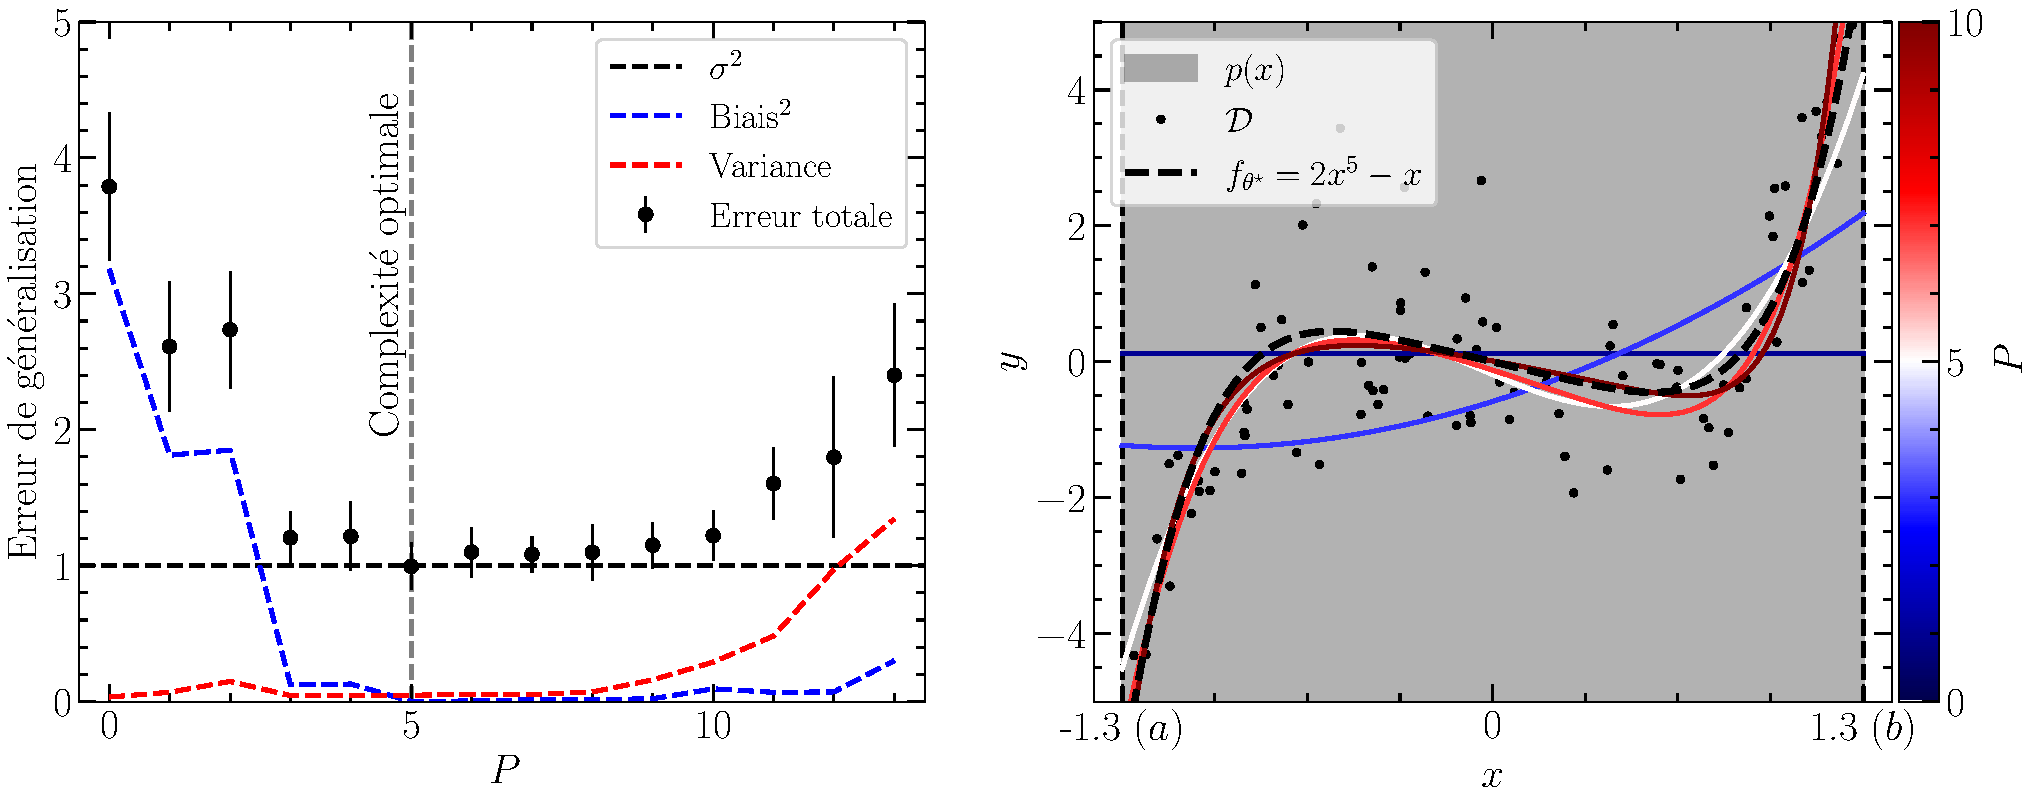
\includegraphics[width=\textwidth]{notebooks/bias_variance.pdf}
        \caption{Compromis classique entre le biais et la variance d'un algorithme d'apprentissage machine pour l'ajustement d'un polynôme de degré $P$ sur les données générées de la 
        loi $f_{\theta^\star} = 2x^5 - x$.}
        \label{fig:bias_variance}
\end{figure}

Le comportement de cette erreur 
peut être compris intuitivement par une décomposition de l'erreur totale en termes de l'erreur irréductible du problème 
$\sigma^2$, du biais 
\begin{equation}
        \mathrm{Biais}(f_{\theta}(x)) = \mathbb{E}_{\mathcal{D}}\left[ f_{\theta}(x)\right] - f_{\theta^{\star}}(x)\, ,
\end{equation} 
et de la variance d'un algorithme d'apprentissage machine 
\begin{equation}
       \mathrm{Variance}(f_\theta(x)) = \mathbb{E}_{\mathcal{D}}\left[ \big(f_{\theta}(x) - \mathbb{E}_{\mathcal{D}}\left[f_{\theta}(x) \right] \big)^2 \right]\, .
\end{equation} 
Lorsque le modèle n'est pas suffisamment complexe pour capturer l'ensemble des points de données, la solution est biaisée par le choix du modèle (courbes bleues de la 
figure \ref{fig:bias_variance}). Le biais est la principale cause du phénomène appelé le \textit{sous-ajustement}, soit lorsqu'un algorithme d'apprentissage n'est pas suffisamment 
flexible pour modéliser une certaine distribution $\mathcal{D}$. Lorsque le modèle est trop complexe, 
le modèle est aussi trop flexible et on observe un phénomène de \textit{sur-ajustement} (courbes rouges de la figure \ref{fig:bias_variance}). 
C.-à-d.~que les modèles entraînés se spécialisent à leur ensemble d'entraînement. 
L'erreur moyenne de généralisation augmente puisque la solution trouvée par l'algorithme d'apprentissage dépend fortement de l'ensemble d'entraînement $\mathcal{D}$, 
qui ne sera pas nécessairement représentatif de la loi générative implicite $f_{\theta^{\star}}(x)$. La variance domine l'erreur 
de généralisation dans ce régime.

Dans tous les cas, l'erreur minimale correspond à $\sigma^2$, soit le niveau d'erreur irréductible à un problème donné. 
Ce niveau d'erreur ne peut être atteint que lorsque la complexité du modèle est environ égale à la complexité de la loi 
générative. En général, on s'attend donc à ce qu'un niveau de complexité optimal existe pour un problème donné. 
La décomposition de l'erreur en termes du biais et de la variance est une méthode pour découvrir cette complexité. 
Cette procédure fonctionne certainement pour le problème de régression décrit dans cette section, mais elle n'est pas garantie de fonctionner en général. 
En effet, le biais et la variance d'une fonction sont des quantités presque impossibles à calculer en général, puisqu'on doit calculer l'espérance d'une fonction 
apprise par $\mathcal{G}$ étant donné différentes réalisations de $\mathcal{D}$.

Ce qui nous concerne maintenant est une discussion sur la sélection du modèle lorsqu'on doit apprendre 
une fonction sur des données multidimensionnelles, soit le cas plus général d'apprentissage machine.


\subsection{La séparabilité linéaire}
C'est lorsqu'on cherche à construire une série entière pour des données multidimensionnelles qu'on réalise que la tâche 
est exponentiellement plus difficile que le cas unidimensionnel. Considérons le cas le plus simple, soit une fonction 
$f_\theta : \mathbb{R}^2 \rightarrow \mathbb{R}$. Dans ce cas, la série entière la plus générale est
\begin{equation}\label{eq:multidim expansion}
        f_\theta(x_1, x_2) = \theta^{(0)} 
        + 
        \begin{bmatrix}
                \theta^{(1)}_0 & \theta^{(1)}_1 
        \end{bmatrix}
        \begin{bmatrix}
               x_1 \\
               x_2
        \end{bmatrix}
        +
        \begin{bmatrix}
                x_1 & x_2 
        \end{bmatrix}
        \begin{bmatrix}
                \theta^{(2)}_{11} & \theta^{(2)}_{12} \\
                \theta^{(2)}_{21} & \theta^{(2)}_{22}
        \end{bmatrix}
        \begin{bmatrix}
                x_1 \\ x_2
        \end{bmatrix}
        + \dots
\end{equation} 
Contrairement à la section précédente, on doit introduire un tenseur de rang $p$ pour le $p^{\text{ième}}$ terme dans la série entière, 
soit $2^p$ nouveaux paramètres qui doivent être ajustés. Dans le cas général $f_\theta: \mathbb{R}^n \rightarrow \mathbb{R}^m$,
on doit plutôt introduire $n^pm$ nouveaux paramètres pour chaque terme ajouté dans la série. 
La complexité du modèle augmente de façon exponentielle en fonction du degré $P$ du modèle.
Ce comportement est radicalement différent du cas présenté à la section précédente, où la complexité du modèle augmentait de façon linéaire en fonction de $P$. 
Dû à ce fait, une série entière n'est pas une approche valide pour construire des modèles complexes en haute dimension; 
le nombre de paramètres qu'on doit introduire devient rapidement intraitable.

\begin{figure}[ht!]
        \centering
        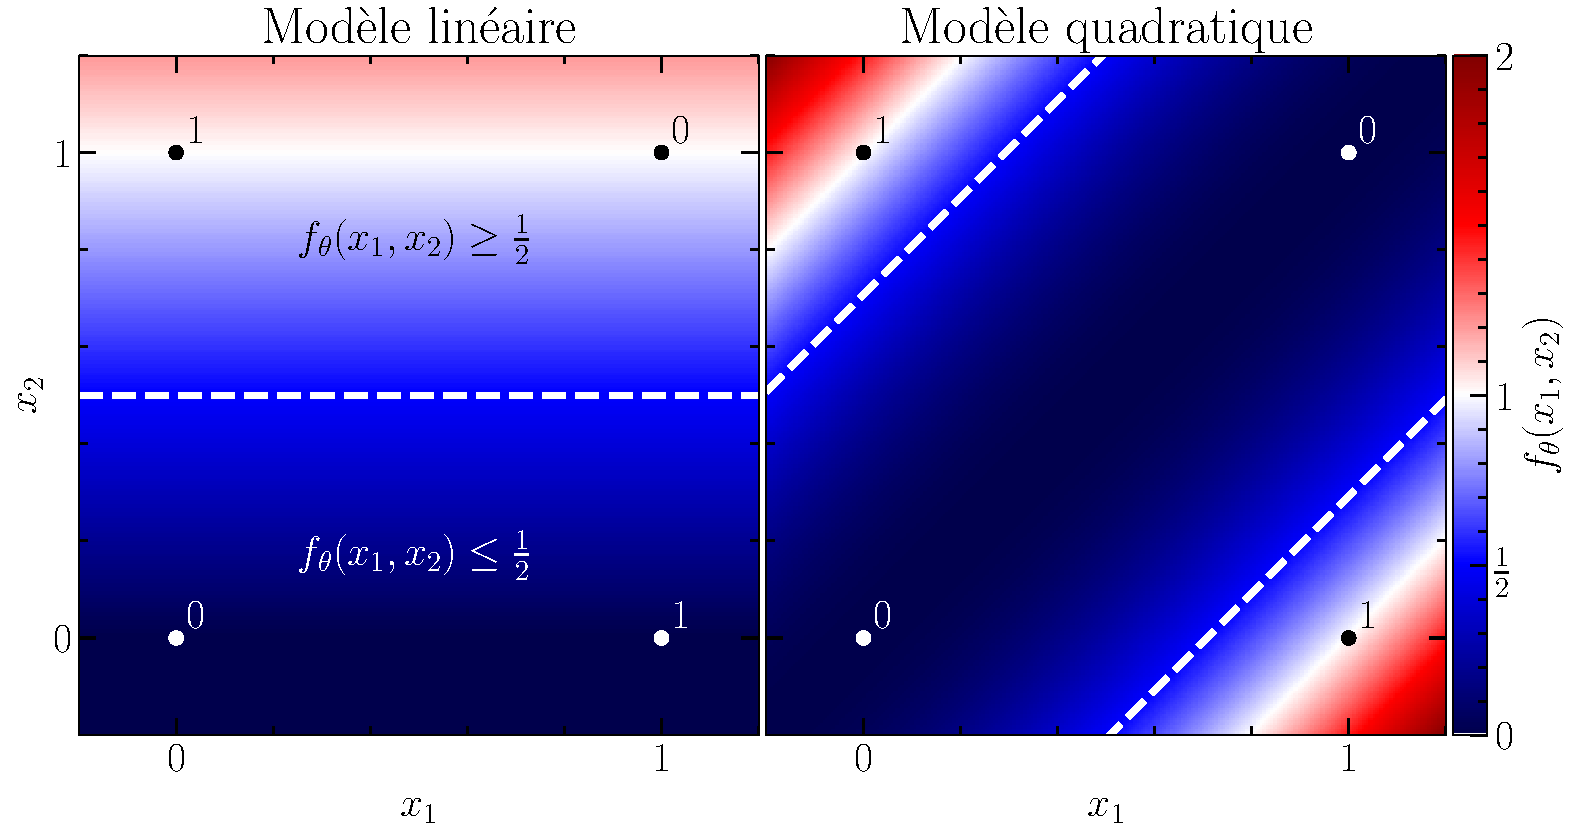
\includegraphics[width=0.7\textwidth]{notebooks/xor.pdf}
        \caption{Comparaison d'un modèle linéaire et d'un modèle quadratique pour le problème XOR.}
        \label{fig:xor}
\end{figure}

Malgré cela, on peut explorer l'application d'un modèle comme \eqref{eq:multidim expansion} dans le but de développer 
une intuition géométrique qui servira à introduire la prochaine méthode pour complexifier $f_\theta$.
On considère l'exemple le plus simple qui requiert un modèle quadratique, 
soit la fonction logique OU exclusive (mieux connue comme XOR dans le jargon de la science informatique). Cette fonction logique peut être 
décrite de façon exhaustive avec la table \ref{tab:xor}.
\begin{table}[ht!]
        \centering
        \begin{tabular}{ccc}
                $x_1$ & $x_2$ & $f_{\theta^{\star}}(x_1, x_2)$  \\\hline
                0 & 0 & 0 \\ 
                0 & 1 & 1 \\
                1 & 0 & 1 \\
                1 & 1 & 0 \\\hline
        \end{tabular}
        \caption{Fonction logique XOR.}
        \label{tab:xor}
\end{table}


%Un ajustement de paramètres d'une fonction linéaire
Ce problème ne peut pas être résolu par une fonction linéaire puisque les 4 contraintes du problème ne sont pas linéairement séparables.
Plus spécifiquement, on ne peut pas construire de plan qui sépare les points qui correspondent à $f_{\theta^{\star}} = 0$ des points 
qui correspondent à $f_{\theta^{\star}} = 1$. Le panneau gauche de la figure \ref{fig:xor} montre le modèle linéaire
\begin{equation}\label{eq:sol1}
        f_{\hat{\theta}}(x_1, x_2) = \begin{bmatrix}0 & 1 \end{bmatrix} \begin{bmatrix} x_1 \\ x_2 \end{bmatrix} = x_2\, 
\end{equation}
pour illustrer cet argument, où on montre comment le plan $f_{\hat{\theta}}(x_1, x_2) = \frac{1}{2}$ (ligne pointillée blanche) 
n'est pas en mesure de séparer les 4 contraintes linéairement.
De plus, aucune rotation ou translation (et en général aucune transformation affine) de ce modèle 
ne peut séparer les points $0$ et $1$ linéairement. 
Au mieux, on pourrait retrouver 3 contraintes avec le modèle $f_{\hat{\theta}} = x_1 - x_2$. Toutefois, on ne peut pas retrouver 
les 4 contraintes puisque l'ensemble des modèles linéaires ne contient pas la fonction XOR.
%On notera que le modèle n'est pas optimal en termes de l'erreur moyenne quadratique puisque $f_\theta(x_1, x_2) = \frac{1}{2}$ possède une erreur inférieure (et optimale), 
%bien que ce dernier ne recouvre aucune contrainte. 

Pour résoudre le problème, on doit introduire le terme de second degré dans la série de puissances \eqref{eq:multidim expansion}. 
Cet ensemble de fonctions contient une infinité de solutions au problème XOR. Le panneau de droite de la figure \ref{fig:xor} 
illustre la solution particulière
\begin{equation}\label{eq:sol quad}
        f_{\hat{\theta}}(x_1, x_2) = \begin{bmatrix} x_1 & x_2 \end{bmatrix} \begin{bmatrix} 1 & -1 \\ -1 & 1 \end{bmatrix} \begin{bmatrix} x_1 \\ x_2 \end{bmatrix} = (x_1 - x_2)^2\,
\end{equation} 
qui recouvre parfaitement les 4 contraintes du problème XOR. Il est intéressant de noter que 
cette solution possède une quantité caractéristique, $h = (x_1 - x_2)^2$, qui est linéairement séparable. En effet, 
on peut tracer un plan $h = \frac{1}{2}$ qui sépare les points $0$ et $1$ dans cet espace. 

Cette observation motive l'introduction d'une nouvelle méthode pour complexifier notre modèle. 
Cette méthode devrait minimalement être en mesure de construire un espace caractéristique (de l'anglais \textit{feature space}) 
équivalent à $h = (x_1 - x_2)^2$, soit un espace caractéristique où les contraintes d'un problème donné sont linéairement séparables.
C'est cette quête qui nous mène naturellement à l'apprentissage profond. 


\section{Les réseaux de neurones}\label{sec:app profond}

Les réseaux de neurones ont été introduits par \citet{Rosenblatt1958} comme des circuits analogues à des circuits biologiques 
de neurones. L'espoir était de mieux comprendre comment les systèmes biologiques sont en mesure de percevoir 
leur environnement; comment l'information est apprise, préservée, remémorée et finalement comment ces systèmes sont 
en mesure de réfléchir, soit prendre en compte toute l'information à leur disposition (perception et mémoire) 
pour dicter ou influencer un comportement. Il s'avère toutefois que ces circuits ont des propriétés qui les rend 
particulièrement intéressants dans le contexte de l'apprentissage machine. 
Ce sont ces propriétés qui nous concernent dans cette section.

\begin{figure}[H]
 \centering
\begin{tikzpicture}
\tikzset{cnode/.style={circle, draw=black, thick, minimum size=0.8cm}}
\node at (-4, 0) {Domaine};
\foreach \i in {0,...,1}
{
        \node[cnode] (x\i) at (\i, 0) {};
}
\node at (-4, -2.75) {Espace};
\node at (-4, -3.25) {caractéristique};

\node at (4.2, -1.75) {Largeur};
\node[rotate=-90] at (3.85, -3.25) {Profondeur};
\draw[-latex, very thick] (3.5, -2) -- (3.5, -4);
\draw[-latex, very thick] (3.5, -2) -- (5.5, -2);
\foreach \i in {0,...,4}
{
        \node[cnode] (z\i) at (\i-1.5, -2) {};
}
\foreach \i in {0,...,4}
{
        \node[cnode] (h\i) at (\i-1.5, -4) {};
}
\node at (-4, -6) {Image};
\node[cnode] (y) at (0.5, -6) {};
\foreach \i in {0,...,1}
{
        \foreach \j in {0,...,4}
        {
                \draw[-latex, thin] (x\i) to (z\j);
        }
}
\foreach \i in {0,...,4}
{
        \foreach \j in {0,...,4}
        {
                \draw[-latex, thin] (z\i) to (h\j);
        }
}
\foreach \j in {0,...,4}
{
        \draw[-latex, thin] (h\j) to (y);
}
\end{tikzpicture}
\caption{Illustration d'un réseau de neurones avec deux couches latentes qui constituent son espace caractéristique.}
\label{fig:mlp}
\end{figure}

La structure mathématique d'un réseau de neurones est généralement introduite à l'aide d'un graphe acyclique, 
tels qu'illustré à la figure \ref{fig:mlp}. Une description tout à fait équivalente de ces réseaux est la  
composition de fonctions
\begin{equation}\label{eq:composition}
        f_\theta(\mathbf{x}) = (f^{(P)}_\theta \circ f^{(P-1)}_\theta \circ \dots \circ f^{(1)}_\theta)(\mathbf{x})\, .
\end{equation} 
Les couches du réseau (de l'anglais \textit{layer}), $f_\theta^{(i)}: \mathbb{R}^{n} \rightarrow \mathbb{R}^{m}$, sont formées de deux composantes essentielles, 
soit une transformation affine $\mathbf{W}\mathbf{z} + \mathbf{b}$ et une fonction non linéaire $\sigma: \mathbb{R} \rightarrow  \mathbb{R}$ 
(aussi appelée fonction d'activation)
\begin{equation}\label{eq:mlp layer}
        f^{(i)}_\theta(\mathbf{z}) = \sigma( \mathbf{W}^{(i)} \mathbf{z} + \mathbf{b}^{(i)})\, .
\end{equation} 
On note $\mathbf{W} \in \mathbb{R}^{m \times n}$, une matrice de poids (de l'anglais \textit{weights}), et 
$\mathbf{b} \in \mathbb{R}^{m}$, un vecteur de biais (de l'anglais \textit{bias}, à ne pas confondre avec le biais statistique mentionné précédemment). 
Dans cette expression, il est sous-entendu que la fonction 
d'activation, $\sigma$, s'applique identiquement sur les $m$ éléments du vecteur $\mathbf{W} \mathbf{z} + \mathbf{b}$. 

Individuellement, 
la transformation affine et la fonction d'activation ne sont pas en mesure de résoudre des problèmes comme XOR. En effet, 
une transformation affine préserve les lignes parallèles d'un espace vectoriel, de sorte 
qu'un ensemble de points qui n'est pas linéairement séparable le restera après une transformation affine. 
D'un autre côté, comme une fonction d'activation agit directement sur les coordonnées, ce type de fonction n'est 
pas en mesure de construire une quantité caractéristique qui mélange les coordonnées 
comme celle trouvée à la section précédente. 

C'est l'application combinée de ces deux ingrédients qui permet minimalement de résoudre un problème comme XOR. Par exemple, 
considérons la fonction d'activation traditionnelle $\mathrm{ReLU}$ (inspirée des neurones biologiques)
\begin{equation}
        \mathrm{ReLU}(x) = 
        \begin{cases}
                x & x \geq 0 \\
                0 & x < 0
        \end{cases}
        =
        \max(0, x), \hspace{1cm} x \in \mathbb{R}
\end{equation}
Pour résoudre le problème XOR, on introduit une seule couche cachée, $f_\theta^{(1)}$, dans le réseau de neurones
\begin{equation}
        f_\theta = \mathbf{W}(f^{(1)}_\theta(\mathbf{x})) + \mathbf{b}\, .
\end{equation} 
La dernière couche du réseau est une transformation affine seulement puisqu'on s'attend à ce que la couche cachée $f^{(1)}_\theta$ puisse 
construire un espace caractéristique qui sépare linéairement les contraintes du problème. Il s'avère que cette construction 
admet la solution suivante
\begin{equation}\label{eq:sol2}
        f_{\hat{\theta}}(x_1, x_2) =
        \begin{bmatrix}
                1 & 1 
        \end{bmatrix}
        \mathrm{ReLU}\left(  
        \begin{bmatrix}
        1 & -1 \\ -1 & 1     
        \end{bmatrix}
        \begin{bmatrix}
                x_1 \\ x_2
        \end{bmatrix}
        \right)
        = \max(0,\, x_1 - x_2) + \max(0,\, x_2 - x_1)\, ,
\end{equation}
où la transformation affine de la couche cachée est la même que celle trouvée dans la section précédente. Pour comprendre intuitivement 
le rôle de chaque composante de ce réseau, la figure \ref{fig:xor2} illustre comment les opérations séquentielles du réseau de neurones \eqref{eq:sol2} 
transforment l'espace du problème vers un espace caractéristique linéairement séparable (identifiable par une droite pointillée).

\begin{figure}[ht!]
\centering
\begin{tikzpicture}
\begin{scope}[shift={(-4,0)}]
        \node[circle, fill=blue, minimum size=5pt, inner sep=0pt] at (1, 1) {};
        \node[circle, fill=blue, minimum size=5pt, inner sep=0pt] at (0, 0) {};
        \node[circle, fill=red, minimum size=5pt, inner sep=0pt] at (0, 1) {};
        \node[circle, fill=red, minimum size=5pt, inner sep=0pt] at (1, 0) {};
        \node[color=red] at (1.2, .2) {$1$};
        \node[color=blue] at (1.2, 1.2) {$0$};
        \node[color=red] at (.2, 1.2) {$1$};
        \node[color=blue] at (.2, .2) {$0$};
        \draw[-latex] (0, -1.5) -- (0, 1.5) node[at end, left] {$x_2$};
        \draw[-latex] (-1.5, 0) -- (1.5, 0) node[at end, below] {$x_1$};
\end{scope}
\draw[-latex] (-3, -1.25) .. controls +(.5, -.5) and +(-.5, -.5) .. (-1, -1.25) node[below, midway] {Transformation affine};

\begin{scope}[shift={(0,0)}]
        \node[circle, fill=red, minimum size=5pt, inner sep=0pt] at (1, -1) {};
        \node[circle, fill=blue, minimum size=5pt, inner sep=0pt] at (0, 0) {};
        \node[circle, fill=red, minimum size=5pt, inner sep=0pt] at (-1, 1) {};
        \draw[-latex] (0, -1.5) -- (0, 1.5) node[at end, left] {$h_2$};
        \draw[-latex] (-1.5, 0) -- (1.5, 0) node[at end, below] {$h_1$};
\end{scope}
\draw[-latex] (1, -1.25) .. controls +(.5, -.5) and +(-.5, -.5) .. (3, -1.25) node[below, midway] {ReLU};

\begin{scope}[shift={(4,0)}]
        \node[circle, fill=red, minimum size=5pt, inner sep=0pt] at (1, 0) {};
        \node[circle, fill=blue, minimum size=5pt, inner sep=0pt] at (0, 0) {};
        \node[circle, fill=red, minimum size=5pt, inner sep=0pt] at (0, 1) {};
        \draw[-latex] (0, -1.5) -- (0, 1.5) node[at end, left] {$h'_2$};
        \draw[-latex] (-1.5, 0) -- (1.5, 0) node[at end, below] {$h'_1$};
        \draw[dashed, thick] (-1, 1.5) -- (1.5, -1);
\end{scope}

\draw[-latex] (5, -1.25) .. controls +(.5, -.5) and +(-.5, -.5) .. (7, -1.25) node[below, midway] {Transformation affine};

\begin{scope}[shift={(8,0)}]
        \node[circle, fill=red, minimum size=5pt, inner sep=0pt] at (1, 0) {};
        \node[circle, fill=blue, minimum size=5pt, inner sep=0pt] at (0, 0) {};
        \draw[-latex] (-1.5, 0) -- (1.5, 0) node[at end, below] {$f_{\hat{\theta}}$};
        \draw[dashed, thick] (0.5, 1) -- (0.5, -1);
\end{scope}
        
\end{tikzpicture}
\caption{Illustration d'une transformation du problème XOR vers un espace caractéristique linéairement séparable par un réseau de neurones.}
\label{fig:xor2}
\end{figure}

L'espace caractéristique des réseaux de neurones est la source de leur flexibilité. Le théorème d'approximation universel 
\citep{Cybenko1989,Hornik1991} stipule 
qu'un réseau avec une seule couche cachée d'une largeur suffisante (dimension de l'espace caractéristique) peut représenter 
n'importe quelle fonction continue.
Il est possible d'obtenir une limite supérieur pour la largeur du réseau de neurones par des arguments géométriques dans des cas simples comme XOR.
En général, un problème de classification binaire avec $N$ points de données (4 dans le cas de XOR) est toujours linéairement séparable dans 
un espace caractéristique de dimensions $D$ tels que $D \geq N - 1$. 

Ce critère provient du théorème de \citet{Cover1965} et de la dimension de Vapnik-Chervonenkis d'un classificateur linéaire \citep{Vapnik1971,Vapnik1995}. 
La probabilité qu'un ensemble de $N$ points soit linéairement séparable augmente 
considérablement en fonction de la dimension de l'espace, et atteint $p = 1$ lorsque $D \geq N -1$.
Pour le problème XOR, on a trouvé que $D=2$ admettait une solution. 
%En général, le théorème de Cover est une limite supérieure sur la dimensionnalité de l'espace caractéristique, 
%et garantit qu'un réseau de neurones à une couche peut résoudre un problème de classification binaire arbitrairement complexe. 
Il est assez rare que la limite supérieure $D \geq N -1 $ soit 
atteinte puisque les données réelles tendent à se regrouper sur des variétés de basses dimensions. 
Néanmoins, spécifier une couche cachée suffisamment large peut devenir rapidement intraitable dans certaines situations, 
particulièrement en hautes dimensions. C'est un problème similaire à celui rencontré à la section précédente avec la série entière. 
La prochaine section introduira une stratégie générale pour contourner ce problème, ainsi qu'une application spécifique aux réseaux de neuronnes 
convolutifs utilisés pour le traitement d'images.

Avant de poursuivre, on doit mentionner que les réseaux de neurones 
ne sont pas des fonctions linéaires en fonction de leurs paramètres (contrairement à la série entière). 
Ainsi, l'apprentissage profond introduit un problème d'optimisation non linéaire, soit un problème avec 
potentiellement plusieurs minimas secondaires et une géométrie non triviale.
Les algorithmes d'apprentissage modernes
sont largement équipés pour résoudre ce genre de problème grâce à l'introduction des dérivées automatiques et 
des algorithmes de descente de gradient stochastiques. Voir le livre de référence de \citet{Goodfellow2016} 
pour une discussion plus détaillée de ce sujet.

%Je termine finalement ce chapitre avec une très courte introduction sur les réseaux neuronaux convolutifs. Ces réseaux sont utilisés 
%extensivement dans les deux prochains chapitres étant donné que le problème étudié dans ce mémoire nécessite l'introduction de réseaux 
%spécialisés pour le traitement d'image. 

\section{Les réseaux de neurones convolutifs}\label{sec:cnn}
Le traitement d'image pose un problème sérieux à l'apprentissage machine en raison de la dimensionalité du problème. 
Une image est généralement décrite par 3 dimensions qui décrivent respectivement la hauteur ($H$), la largeur ($L$) et le nombre de canaux de couleurs ($C$). 
La dimensionalité d'une image correspond au nombre total de pixels qui décrivent cette image, soit $C \times H \times L $, 
un nombre qui peut facilement atteindre une valeur de l'ordre de $\mathcal{O}(10^{5})$ en astronomie.

Pour construire une fonction avec un nombre raisonnable de paramètres, on utilise le principe d'équivarience. 
Ce principe est fortement inspiré du principe de la covariance, originellement formulé 
par Einstein, qui stipule qu'une théorie physique devrait être formulée en termes des quantités qui se transforme de façon covariantes 
par rapport à une action du groupe de symétrie de la théorie. Le principe d'équivarience stipule similairement qu'une fonction $f_\theta$ doit se transformer de façon équivariente
sous l'action du groupe de symétrie $G$ du problème à l'étude
\begin{equation}
        \begin{split}
                x &\rightarrow Tx\\
                f_\theta(x) &\rightarrow f'_\theta(Tx) = T'f_\theta(x) \, .
        \end{split}
\end{equation} 
$T, T' \in G$ sont des éléments du groupe de symétrie. $T'$ est la représentation de l'action $T$ dans l'espace vectoriel de l'image de la fonction $f_\theta$.

La convolution est une opération équivariante sous l'effet d'une translation. 
Pour rendre cette observation concrète, prenons l'exemple de la convolution entre le noyau de la convolution $\mathbf{W} \in \mathbb{R}^{m}$ 
et un vecteur $\mathbf{x} \in \mathbb{R}^{n}$
\begin{equation}\label{eq:conv}
        (\mathbf{W} * \mathbf{x})_j = \sum_{i = 0}^{m-1} \mathbf{W}_i\, \mathbf{x}_{j - i}
\end{equation} 
L'effet d'une translation sur le vecteur $\mathbf{x}$ est de modifier l'ordre des indices. On note $T_{w}$ une translation 
qui déplace les indices de la façon suivante: $T_w\mathbf{x}_{j} = \mathbf{x}_{j+w}$. 
Il est sous-entendu que les indices du vecteur $\mathbf{x}$ sont définis $\mathrm{mod}\, n$. 
On peut alors montrer que la convolution \eqref{eq:conv} est une opération équivariante sous l'effet d'une translation 
\begin{equation}
        (\mathbf{W} *(T_w\mathbf{x}))_j = \sum_{i = 0}^{m-1} \mathbf{W}_i\, \mathbf{x}_{j + w - i} = (\mathbf{W} * \mathbf{x})_{j + w} = T_w(\mathbf{W} * \mathbf{x})_{j}
\end{equation} 
Comparé à une transformation affine, le noyau de la convolution requiert beaucoup moins de paramètres pour un niveau comparable d'expressivité. En effet, 
il est souvent justifié de supposer que l'information à extraire du domaine est localement corrélée. 
En supposant que la distance de corrélation est $m< n$, on peut construire un noyau pour la convolution avec $m$ paramètres. C'est un énorme  
avantage comparé à la transformation affine. Cette dernière a besoin, minimalement, de $n$ paramètres pour chaque dimension 
de l'espace caractéristique.

Cet avantage devient significatif lorsqu'on considère des images $\mathbf{x} \in \mathbb{R}^{C \times H\times L}$, soit des tenseurs de rang 3. 
On considère une convolution sur les dimensions spatiales seulement ($H$ et $L$) et on pose ${W \in \mathbb{R}^{C \times c \times h \times \ell }}$. On définit la convolution sur une image 
\begin{equation}
        (\mathbf{W} * \mathbf{x})_{ijk} = \sum_{m=0}^{C-1} \sum_{n=0}^{h-1}\sum_{p=0}^{\ell-1}\mathbf{W}_{minp} \mathbf{x}_{m,j-n,k-p}
\end{equation} 
Les dimensions spatiales du noyau sont généralement choisis tels que $h \ll H$ et $\ell \ll L$ 
puisque l'information pertinente est locale pour les tâches de traitement d'images typiques. Par 
exemple, la taille du noyau $h = \ell = 3 $ est choix commun même lorsque la taille d'une image atteint $H \times L \gtrsim 10^4$. 
L'expressivité d'un réseau de neurones convolutifs \citep{LeCun1995} dépend principalement du nombre de canaux utilisés pour l'espace caractéristique 
et de la profondeur du réseau \citep{Krizhevsky2012}.

Ceci complète donc cette introduction à l'apprentissage machine. Comme l'architecture des réseaux 
de neurones est un sujet qui dépend du problème à l'étude, ce sujet est abordé dans 
les prochains chapitres qui traitent en détails des méthodes utilisées dans ce mémoire.


  \chapter{Apprentissage profond de distributions implicites}\label{chap:intro ml}

\section{Auto-encodeur variationnel}\label{sec:vae}
 
\subsection{Description du modèle}

Les auto-encodeurs variationnels (VAE) ont été introduits par \citet{Kingma2013} comme une approche 
pour inférer approximativement les variables latentes (ou cachées) qui contrôlent un certain processus génératif. 
Leur utilité est particulièrement marquée lorsque ce processus génératif est défini implicitement par un échantillon de données, 
soit un cas où la forme fonctionnelle de la distribution n'est pas connue a priori.
Dans cette section, j'introduis 
les concepts principaux reliés à ce type de modélisation. 
Le lecteur peut aussi se référer au livre blanc de \citet{Kingma2019}.

On définit $\mathbf{z}\in \mathbb{R}^{h}$ comme une variable latente et $\mathbf{x}\in \mathbb{R}^{m}$ ($m > h$) 
comme un exemple d'un échantillon de donnée $\mathcal{D} = \{\mathbf{x}^{(i)}\}_{i=1}^{N}$. 
Notre objectif est de modéliser la distribution, $p(\mathbf{x})$, implicitement décrite par notre échantillon. 
On définit une approximation de cette distribution, $p_\theta(\mathbf{x})$, caractérisée par une liste de paramètres $\theta$,
et on définit un processus génératif modélisé par la conditionnelle sur la variable cachée $p_\theta(\mathbf{x \mid \mathbf{z}})$. 
Déterminer $p_\theta$ directement est généralement difficile, voir impossible, si la dimensionnalité de $\mathbf{x}$ est grande 
($\mathrm{dim(\mathbf{x}}) \gtrsim 10^{4}$ pour des images). 
Pour contourner ce problème, on introduit une distribution variationnelle, $q_\phi(\mathbf{z} \mid \mathbf{x})$, dont le rôle est 
d'inférer la variable latente $\mathbf{z}$ associée à $\mathbf{x} \sim p_\theta(\mathbf{x} \mid \mathbf{z})$. 
En d'autres mots, $q_\phi(\mathbf{z} \mid \mathbf{x})$ est une approximation variationnelle de la distribution a posteriori $p_\theta(\mathbf{z} \mid \mathbf{x})$.
La notion de distance entre ces deux distributions est mesurée par la divergence de Kullback-Leibler $D_{\mathrm{KL}}(\cdot \KL \cdot) \geq 0$: 
\begin{align}
        \nonumber
       D_{\mathrm{KL}}(q_\phi(\mathbf{z} \mid \mathbf{x}) \KL  p_\theta (\mathbf{z} \mid \mathbf{x})) 
       &= \mathbb{E}_{q_\phi(\mathbf{z} \mid \mathbf{x})} \bigg[\log q_\phi(\mathbf{z} \mid \mathbf{x}) - \log p_\theta (\mathbf{z} \mid \mathbf{x}) \bigg]  \\
       \nonumber
       &= \mathbb{E}_{q_\phi(\mathbf{z} \mid \mathbf{x})} \bigg[\log q_\phi (\mathbf{z} \mid \mathbf{x}) -\log \frac{p_\theta(\mathbf{z}, \mathbf{x})}{p_\theta(\mathbf{x})} \bigg]  \\
       \label{eq:KL}
       &= \log p_\theta (\mathbf{x}) - \underbrace{\mathbb{E}_{q_\phi(\mathbf{z} \mid \mathbf{x})} \bigg[\log p_\theta(\mathbf{z}, \mathbf{x}) - \log q_\phi (\mathbf{z} \mid \mathbf{x}) \bigg]}_{\equiv \mathcal{L}_{\phi,\theta}(\mathbf{x})} \, .
\end{align} 

On remarque par cette manipulation que la distance $D_{\mathrm{KL}}$, en plus de mesurer la distance entre 
les deux distributions a posteriori (par définition), mesure aussi la différence entre le terme 
$\mathcal{L}_{\phi,\theta}(\mathbf{x})$, qu'on nomme limite inférieure sur l'évidence (de l'anglais 
\textit{evidence lower bound}: ELBO), et la distribution marginale qu'on cherche à modéliser, $p_\theta(\mathbf{x})$. 
L'objectif d'un modèle VAE est de maximiser la ELBO, $\mathcal{L_{\phi,\theta}}$. 
En observant l'équation \eqref{eq:KL}, on réalise que cet objectif 
nous permet d'améliorer le modèle d'inférence et le processus génératif simultanément.
En effet, la divergence KL est 
une quantité positive, donc maximiser la ELBO a pour effet de
\begin{enumerate}
        \item maximiser $p_\theta(\mathbf{x}) = \int p_{\theta}(\mathbf{x} \mid \mathbf{z}) p_{\theta}(\mathbf{z}) d\mathbf{z}$, ce qui suit de l'inégalité
                $\log p_\theta \geq \mathcal{L}_{\phi,\theta}(\mathbf{x})$ (améliore le processus génératif);
        \item minimiser $D_{\mathrm{KL}}(q_\phi(\mathbf{z} \mid \mathbf{x}) \KL  p_\theta (\mathbf{z} \mid \mathbf{x})) = \log p_\theta(\mathbf{x}) - \mathcal{L}_{\phi,\theta}(\mathbf{x})$ (améliore le processus d'inférence de $\mathbf{z}$).
\end{enumerate}

\begin{figure}[H]
        \centering
        \begin{tikzpicture}
                \node[circle, draw=black, minimum size=1cm] (z) at (0, 3) {$\mathbf{z}$};
                \node[circle, draw=black, minimum size=1cm] (x) at (0, 0) {$\mathbf{x}$};
                \draw[-{Latex[scale=2]}] (z) to (x);
                \draw[-{Latex[scale=2]}, in=225, out=135, dashed] (x) to (z);
                \node (phi) at (-2.5, 2.5) {$\phi$};
                \node (theta) at (2.5, 2.5) {$\theta$};
                \draw[rounded corners=0.5cm] (-1.5, -0.7) rectangle (1.5, 3.7);
                \draw[-{Latex[scale=2]}] (theta) to node[sloped, midway, below=5pt, fill=white, rectangle, draw=white, opacity=.8, text opacity=1] {$p_\theta(\mathbf{\mathbf{x} \mid \mathbf{z}})$} (x);
                \draw[-{Latex[scale=2]}] (theta) to node[sloped, midway, above=5pt, fill=white, rectangle, draw=white, opacity=.8, text opacity=1] {$p_\theta(\mathbf{z})$} (z);
                \draw[-{Latex[scale=2]}, dashed] (phi) to node[sloped, midway, above=5pt, fill=white, rectangle, draw=white, opacity=.8, text opacity=1] {$q_\phi(\mathbf{z} \mid \mathbf{x})$} (z); 
                \node at (1, -0.5) {$N$};
        \end{tikzpicture}
        \caption{Modèle graphique d'un VAE. Les flèches pleines indiquent le processus génératif, alors que les flèches pointillées indiquent le processus d'inférence.}
        \label{fig:vae encoder}
\end{figure}

\subsection{Le truc de la reparamétrisation}
Le gradient de la ELBO par rapport aux paramètres variationnels, $\grad_{\phi,\theta}\mathcal{L}_{\phi,\theta}(\mathbf{x})$, 
est une quantité qu'on doit calculer pour faire usage d'algorithmes comme la descente de gradient stochastique 
pour maximiser la ELBO en termes de $\phi$ et $\theta$. 
Or, la liste de paramètres $\phi$ apparait dans la distribution de prélèvement pour calculer 
l'espérance mathématique $\mathbb{E}_{q_\phi(\mathbf{z} \mid \mathbf{x})}$ dans la ELBO \eqref{eq:KL}.
Cette opération n'a pas de dérivée formelle en termes de $\phi$. 

Pour résoudre ce problème, on utilise le truc de reparamétrisation \citep{Kingma2013}, 
qui consiste à exprimer la variable aléatoire latente $\mathbf{z} \sim q_\phi (\mathbf{z} \mid \mathbf{x})$ 
comme la transformation différentiable et inversible d'une variable aléatoire auxiliaire $\boldsymbol{\epsilon}$.
On considère le cas où $q_\phi(\mathbf{z} \mid \mathbf{x})$ et $p(\boldsymbol{ \epsilon})$ 
font partie de la famille gaussienne isotropique
\begin{align}
        \label{eq:p epsilon}
        \boldsymbol{\epsilon} &\sim \mathcal{N}(0, \bbone)\, ;\\
        %\label{eq:q phi}
        %q_\phi(\mathbf{z} \mid \mathbf{x}) &= \mathcal{N}(\boldsymbol{ \mu}_\phi (\mathbf{x}),\, \bbone \boldsymbol{\sigma}_\phi^{2}(\mathbf{x}))\, ;\\
        \label{eq:reparametrisation}
        \mathbf{z} &= \boldsymbol{\mu}_\phi + \boldsymbol{ \sigma}_\phi \odot \boldsymbol{ \epsilon}\, , 
\end{align} 
de sorte que 
\begin{equation}\label{eq:q phi}
        \mathbf{z} \sim q_\phi(\mathbf{z} \mid \mathbf{x}) = \mathcal{N}(\boldsymbol{ \mu}_\phi (\mathbf{x}),\, \bbone \boldsymbol{\sigma}_\phi^{2}(\mathbf{x}))\, .
\end{equation} 
$\odot$ symbolise le produit d'Hadamard, ou encore le produit élément par élément de vecteurs.
La reparamétrisation fait en sorte que les paramètres variationnels ne participent plus au processus de prélèvement, 
maintenant pris en charge par $\boldsymbol{ \epsilon} $.
Cette propriété est cruciale, car elle nous permet de prendre le gradient de la ELBO \eqref{eq:KL}. 
En effet, on peut maintenant échanger les opérateurs $\grad_{\phi,\theta}$ et ${\mathbb{E}_{q_\phi(\mathbf{z} \mid \mathbf{x})} = \mathbb{E}_{p(\boldsymbol{ \epsilon})}}$,
ce qui nous permet d'appliquer le gradient à l'intérieur de l'espérance mathématique.
De plus, $\phi$ décrit maintenant une fonction générique dont le rôle est d'inférer les 
paramètres de la distribution $q_\phi(\mathbf{z} \mid \mathbf{x})$
\begin{equation}
        \begin{aligned}
                f_\phi: \mathbb{R}^{m} &\rightarrow \mathbb{R}^{h} \times \mathbb{R}^{h}\\ \mathbf{x} &\mapsto (\boldsymbol{\mu},\, \log \boldsymbol{\sigma}^{2})
        \end{aligned}
\end{equation} 
En pratique, on peut construire une approximation de 
cette fonction avec un réseau de neurones convolutif lorsque $\mathbf{x}$ est une image, 
suivant le principe d'approximation universelle \citep{Cybenko1989,Hornik1991}. 

L'objectif d'entraînement de la fonction $f_\phi$ nécessite de manipuler la ELBO pour obtenir une 
divergence KL
\begin{align}
        \mathcal{L}_{\phi,\theta}(\mathbf{x}) &= \mathbb{E}_{q_\phi(\mathbf{z} \mid \mathbf{x})} \bigg[ \log p_\theta(\mathbf{z}, \mathbf{x}) - \log q_\phi (\mathbf{z} \mid \mathbf{x}) \bigg]\, ; \\
        \label{eq:final elbo}
         \implies \mathcal{L}_{\phi,\theta}(\mathbf{x})  &= 
         \underbrace{\mathbb{E}_{q_\phi(\mathbf{z} \mid \mathbf{x})} \bigg[ \log p_\theta(\mathbf{x} \mid \mathbf{z})\bigg]}_{\text{terme de reconstruction}}
         + \underbrace{
                \mathbb{E}_{q_\phi(\mathbf{z} \mid \mathbf{x})} \bigg[\log p_{\theta}(\mathbf{z}) - \log q_\phi (\mathbf{z} \mid \mathbf{x}) \bigg]
        }_{\equiv -D_{\mathrm{KL}}(q_\phi(\mathbf{z} \mid \mathbf{x})\, \KL\, p_\theta(\mathbf{z}))}\, .
\end{align} 
Pour déterminer la forme fonctionnelle de la divergence KL obtenue au second terme du membre droit de l'équation \eqref{eq:final elbo}, 
on stipule a priori que la distribution marginale des variables latentes 
devrait correspondre à une distribution normale isotropique
\begin{equation}\label{eq:latent distribution}
        p_{\theta}(\mathbf{z}) = \mathcal{N}(0, \bbone)
\end{equation}
La KL admet alors une solution fermée étant donné les familles paramétriques stipulées 
pour $p_\theta(\mathbf{z})$ \eqref{eq:latent distribution} et $q_\phi(\mathbf{z} \mid \mathbf{x})$ \eqref{eq:q phi}
\begin{equation}\label{eq:final KL}
        -D_{\mathrm{KL}}(q_\phi(\mathbf{z} \mid \mathbf{x})\, \KL\, p_\theta(\mathbf{z})) =
        \frac{1}{2}\sum_{j=1}^{h} (1 + [\log \boldsymbol{ \sigma}_\phi^{2} ]_j - [\boldsymbol{ \mu}_\phi ]_j - [\boldsymbol{ \sigma}_\phi^{2} ]_j)
\end{equation} 
Une dérivation de ce terme est donnée dans l'annexe B de \citet{Kingma2013}. 
%Cette solution se dérive directement par rapport à $\phi$. 
Le premier terme du membre droit de l'équation \eqref{eq:final elbo} 
est nommé \textit{terme de reconstruction} puisqu'il connecte avec l'objectif des fonctions 
de type auto-encodeur d'apprendre une représentation latente d'un échantillon de données.
La reconstruction s'accomplit en utilisant d'abord le modèle d'inférence 
$\mathbf{z}^{(1:L)} \overset{\mathrm{i.i.d}}{\sim} q_\phi(\mathbf{z} \mid \mathbf{x})$ 
pour obtenir un échantillon de représentations latentes à partir des équations \eqref{eq:p epsilon} à \eqref{eq:reparametrisation}, 
puis en utilisant le modèle génératif $\hat{\mathbf{x}}^{(i)} \sim p_\theta(\mathbf{x} \mid \mathbf{z}^{(i)})$ pour obtenir 
un échantillon de reconstructions $\mathbf{\hat{x}}^{(1:L)}$ de l'exemple originel $\mathbf{\mathbf{x}}$. 
Comme on a déjà une variable auxiliaire $\boldsymbol{ \epsilon} $ 
qui se charge de l'aspect génératif du modèle, on peut construire une approximation du 
modèle génératif avec une fonction générique des variables latentes 
${g_\theta: \mathbb{R}^{h} \rightarrow \mathbb{R}^{m};\, \mathbf{z}^{(i)} \mapsto \hat{\mathbf{x}}^{(i)}}$.
Encore une fois, un réseau de neurones convolutif est un choix pratique pour modéliser cette fonction 
dans le cas où $\mathbf{x}$ est une image. En général, on choisit une erreur quadratique moyenne pour modéliser le terme de reconstruction, 
de sorte que
\begin{equation}\label{eq:reconstruction}
        \mathbb{E}_{q_\phi(\mathbf{z} \mid \mathbf{x})} \bigg[
                \log p_\theta(\mathbf{x} \mid \mathbf{z})
        \bigg] 
        = -\frac{1}{L}\sum_{i=1}^{L} \lVert \mathbf{x} - \hat{\mathbf{x}}^{(i)} \rVert_2^{2}
\end{equation} 

\subsection{Principe du goulot d'information}

La fondation théorique des auto-encodeurs variationnels repose sur le principe plus général 
du goulot d'information \citep[BIP, de l'anglais \textit{bottleneck information principle:}][]{Tishby1999}. 
Dans cette sous-section, je décris rapidement certains concepts 
liés à la théorie de l'information de \citet{Shannon1948} 
pour justifier l'introduction d'un multiplicateur de 
Lagrange $\beta$ au terme de régularisation de la ELBO, ${-D_{\mathrm{KL}}(q_\phi(\mathbf{z} \mid \mathbf{x})\, \KL\, p_\theta(\mathbf{z}))}$.
Pour une discussion en profondeur, voir l'excellente revue sur l'utilisation de BIP dans le contexte de l'apprentissage 
machine par \citet{Goldfield2020} et le manuel de référence sur la théorie de l'information par \citet{Cover2006}.
\begin{figure}[thb!]
        \centering
        \resizebox{\linewidth}{!}{
        \begin{tikzpicture}
                \node at (-8, -2.8) {Indice d'un};
                \node at (-8, -3.3) {ensemble des données};
                \node[circle, draw=black, minimum size=1cm] (obj) at (-8, -2) {$Y$}; 
                \node at (-8, 1.4) {Source};
                \node at (-8, 0.9) {d'information};
                \node[circle, draw=black, minimum size=1cm] (x) at (-8, 0) {$X$}; 
                \node at (-4, 1.3) {Encodeur};
                \node[rectangle, draw=black, minimum width=2cm, minimum height=2cm] (encoder) at (-4, 0) {$q_\phi(\mathbf{z} \mid \mathbf{x})$}; 
                \node at (0, 0.9) {Code};
                \node[circle, draw=black, minimum size=1cm] (z) at (0, 0) {$Z$};
                \node[circle, draw=black, minimum size=1cm] (eps) at (0, -2) {$\epsilon$};
                \node at (0, -2.8) {Source de bruit};
                \node[rectangle, draw=black, minimum width=2cm, minimum height=2cm] (decoder) at (4, 0) {$p_\theta(\mathbf{x} \mid \mathbf{z})$};
                \node at (4, 1.3) {Décodeur};
                \node[circle, draw=black, minimum size=1cm] (xhat) at (8, 0) {$\hat{X}$};
                \node at (8, 0.9) {Reconstruction};
               
                \draw[-latex] (obj) -- (x);
                \draw[-latex] (x) -- node[midway, below] {Message} (encoder);
                \draw[-latex] (encoder) -- node[midway, below] {Signal} (z);
                \draw[-latex] (z) -- node[midway, below] {Signal} (decoder);
                \node at (1.8, -0.8) {reçu};
                \draw[-latex] (decoder) --node[midway, below] {Message} (xhat);
                \node at (6.2, -0.8) {reçu};
                \draw[-latex] (eps) to (z);
        \end{tikzpicture}
}
        \caption{VAE comme un système de transmission d'information.}
        \label{fig:info VAE}
\end{figure}
L'objectif d'un auto-encoder est de construire un code $Z$ d'une longueur minimale qui capture un maximum d'information contenue dans un message $X$. 
Formellement, on utilise l'information mutuelle de Shannon pour mesurer l'information capturée par $Z$ à propos de $X$
\begin{equation}\label{eq:ShannonInfo}
        I(Z ; X) = D_{\mathrm{KL}}\left(p(\mathbf{x}, \mathbf{z}) \KL p(\mathbf{x}) p(\mathbf{z})\right) %= \mathbb{E}_{p(x,z)} \bigg[\log \frac{p(x,z)}{p(x) p(z)}\bigg] %= \sum_{x \in \mathcal{X}} \sum_{z \in \mathcal{Z}} p(x, z) \log \frac{p(x, z)}{p(x) p(z)}.
\end{equation} 
Il est utile de décomposer cet objectif en termes de l'entropie du message $H(X)$ et l'entropie 
conditionnelle de ce message étant donné le code $Z$, $H(X \mid Z)$
\begin{equation}\label{eq:info entropy}
       I(Z; X) = H(X) - H(X \mid Z) 
\end{equation} 
L'entropie est une mesure de l'incertitude dans une variable aléatoire
\begin{equation}\label{eq:entropy}
        H(X) = -\mathbb{E}_{p(\mathbf{x})}\big[\log p(\mathbf{x}) \big] \geq 0\, ,
\end{equation} 
qu'on interprète aussi comme une mesure de la longueur minimale d'un code, $Z$, pour 
transmettre un message, $X$, d'un émetteur à un receveur avec le minimum de perte d'information \citep{Shannon1948,Kolmogorov1965}.
L'entropie conditionnelle $H(X \mid Z)$ est une  mesure de l'incertitude résiduelle étant donné la connaissance du code $Z$. Dans le cas où $Z$ 
détermine complètement le message $X$, alors $H(X \mid Z) = 0$ et l'information mutuelle atteint son maximum $I(Z; X) = H(X)$.
Dans le cas où $Z$ et $X$ sont deux variables aléatoires indépendantes, $H(X \mid Z) = H(X)$ et l'information mutuelle devient nulle.

Déterminer l'auto-encodeur optimal, c.-à-d. celui qui maximise $I(Z;X)$, est un problème mal posé. 
En effet, on pourrait naïvement maximiser l'objectif \eqref{eq:ShannonInfo} avec 
la fonction identité comme auto-encodeur: $f_{\phi,\theta}(X) = \bbone X$, de sorte que $Z = X$ et $I(Z; X) = H(X)$. 
Or, $Z$ n'est pas une représentation pertinente dans ce cas. 
Pour éliminer les solutions non désirées, on introduit une contrainte sur la complexité de \citet{Kolmogorov1965} du code $Z$, c.-à-d. qu'on cherche 
un auto-encodeur qui compresse le message et conserve simultanément 
le maximum d'information possible à propos du message. On introduit l'objectif du goulot d'information \citep{Tishby1999}
\begin{equation}\label{eq:IB}
\begin{aligned}
        \underset{\phi,\theta}{\mathrm{max}}&\,\,I(Z ; X) \\[1ex]
        \text{sujet à}&\,\, I(Z; Y) \leq \alpha\, .
\end{aligned}
\end{equation} 
La contrainte $I(Z; Y) \leq \alpha$ impose à l'auto-encodeur %$p_{\phi,\theta}(\hat{X} \mid X)$
une limite sur l'information mutuelle entre le code 
utilisé pour représenter $X$ et l'identité $Y=i$ de chaque exemple d'un ensemble des données qu'on veut modéliser $\mathcal{D} = \{\mathbf{x}_i \}_{i=1}^{N}$.
Il s'avère que l'objectif de comprimer l'information est intimement lié à l'objectif d'obtenir un sommaire informatif, c.-à-d. qu'un 
code d'une complexité de \citet{Kolmogorov1965} minimale décrit la source d'information de la manière la plus informative possible. Cette connexion 
remarquable est une application concrète du principe du rasoir d'Occam: l'explication adéquate la plus simple est la meilleure explication.

Dans ce qui suit, je m'applique à redériver l'objectif d'un auto-encodeur variationnel suivant les approximations 
proposées par \citet{Alemi2017}. Puis, je termine avec une courte interprétation des VAE sous la lumière du principe du goulot d'information.
On commence par construire une limite variationnelle inférieure sur $I(Z; X)$. 
On assume d'abord la chaîne de Markov $Y \rightarrow X \rightarrow Z$ pour les variables 
aléatoires représentées dans la figure \ref{fig:info VAE}. La chaîne de Markov 
induit la factorisation de la probabilité jointe
\begin{equation}\label{eq:factorisation}
       p(X, Y, Z) = p(X \mid Z) p(Y \mid X) p(X) 
\end{equation} 
où $p(X \mid Z,\, Y) = p(X \mid Z)$ suit du fait que $Z$ et $Y$ sont des variables conditionnellement indépendantes étant donné $X$.
On introduit ensuite un modèle pour l'encodeur,
$q_\phi (Z \mid X)$, soit un système de transmission d'informations par compression. Il 
suit que 
\begin{align}
        I(Z;\, X) &\equiv \mathbb{E}_{p(\mathbf{z},\, \mathbf{x})} \bigg[\log \frac{p(\mathbf{x},\, \mathbf{z})}{p(\mathbf{x}) p(\mathbf{z})} \bigg]\, ;  \\[1.5ex]
        &= \mathbb{E}_{p(\mathbf{x})}\mathbb{E}_{q_\phi(\mathbf{z} \mid \mathbf{x})} \bigg[\log \frac{q_\phi(\mathbf{x} \mid \mathbf{z})}{p(\mathbf{x})} \bigg]\, ;  \\[1.5ex]
                &= -\mathbb{E}_{p(\mathbf{x})}\bigg[\log p(\mathbf{x}) \bigg]  
                + \mathbb{E}_{p(\mathbf{x})}\mathbb{E}_{q_\phi(\mathbf{z} \mid \mathbf{x})} \bigg[\log q_\phi(\mathbf{x} \mid \mathbf{z})\bigg]\, ;  \\[1.5ex]
                \label{eq:maximum info}
                \implies I(Z;\, X)&\geq \mathbb{E}_{p(\mathbf{x})}\mathbb{E}_{q_\phi(\mathbf{z} \mid \mathbf{x})} \bigg[\log p_\theta (\mathbf{x} \mid \mathbf{z})\bigg]\, .
\end{align}
À la dernière ligne, on a éliminé l'entropie du message $H(X)$, puisque c'est une constante strictement positive qui ne dépend pas de $\phi$.
On a aussi introduit l'approximation variationnelle $p_\theta (\mathbf{x} \mid \mathbf{z}) \approx q_\phi (\mathbf{x} \mid \mathbf{z})$ 
pour approximer la distribution a posteriori de l'encodeur (soit le décodeur). Cette approximation est valide dans le contexte où 
on cherche une limite inférieure pour $I(Z; X)$, puisque la divergence KL entre ces deux distributions est strictement positive.
Ensuite, on cherche une borne supérieure au terme de compression $I(Z; Y)$. 
Pour ce qui suit, on remplace $p(Y=i)$ par $\mathbf{x}^{(i)} \sim \mathcal{D}$ pour illustrer avec plus de clarté 
comment le processus génératif de l'indice induit une sélection d'un exemple $\mathbf{x}^{(i)}$ dans l'ensemble 
d'entraînement $\mathcal{D}$. Il suit que 
\begin{align}
        I(Z; Y) &= \mathbb{E}_{\mathbf{x}^{(i)} \sim \mathcal{D}} \mathbb{E}_{q_\phi(\mathbf{z} \mid \mathbf{x}^{(i)})} \bigg[ 
                \log \frac{q_\phi(\mathbf{z} \mid \mathbf{x}^{(i)}) }{q_\phi (\mathbf{z})}        
        \bigg]\, ; \\[1.5ex]
        \label{eq:compression}
        I(Z; Y) &\leq \mathbb{E}_{\mathbf{x}^{(i)} \sim \mathcal{D}} \mathbb{E}_{q_\phi(\mathbf{z} \mid \mathbf{x}^{(i)})} \bigg[ 
                \log \frac{q_\phi(\mathbf{z} \mid \mathbf{x}^{(i)}) }{p_\theta (\mathbf{z})}        
        \bigg]\, , 
\end{align}
où on a introduit l'approximation variationnelle $p_\theta(\mathbf{z}) \approx q_\phi(\mathbf{z})$. 
L'inégalité suit encore une fois 
du fait que la divergence KL entre ces deux distributions est strictement positive.
On finit la dérivation en écrivant l'objectif du goulot d'information \eqref{eq:IB} en introduisant un multiplicateur 
de Lagrange $\beta$ pour le terme $I(Z; Y)$ et en introduisant 
les limites variationnelles \eqref{eq:maximum info} et \eqref{eq:compression}. On ignore  
l'espérance mathématique $\mathbb{E}_{p(\mathbf{x})} = \mathbb{E}_{\mathbf{x}^{(i)} \sim \mathcal{D}}$ pour mieux illustrer la connexion 
avec la ELBO \eqref{eq:final elbo}
\begin{equation}\label{eq:beta VAE}
        \mathcal{L}_{\phi,\theta,\beta}(\mathbf{x}) =  \mathbb{E}_{q_\phi(\mathbf{z} \mid \mathbf{x})} \bigg[\log p_\theta (\mathbf{x} \mid \mathbf{z})\bigg]
        -  \beta  \mathbb{E}_{q_\phi(\mathbf{z} \mid \mathbf{x})} \bigg[ 
                \log q_\phi(\mathbf{z} \mid \mathbf{x})        
                -\log p_\theta(\mathbf{z})
                \bigg]
\end{equation} 
On note qu'on a laissé tomber la constante $\alpha$, car elle ne dépend pas des paramètres $\phi$ et $\theta$, et généralement le paramètre $\beta$ 
n'est pas optimisé directement. $\beta$ est considéré comme un hyperparamètre. 
Je note que l'objectif \eqref{eq:beta VAE} a fait une première apparition dans le travail introduisant les $\beta$-VAE par \citet{Higgins2017}, 
suivant des motivations complètement différentes de celles qu'on a suivies ici. La dérivation accomplie ici 
montre clairement que la ELBO, $\mathcal{L}_{\phi,\theta,\beta}(\mathbf{x})$, est une limite inférieure 
sur $I(Z; X) - \beta I(Z; Y)$, soit l'objectif de maximiser l'information transmise par un auto-encodeur, avec une 
contrainte sur la complexité du code $Z$. En particulier, cette dérivation illumine le choix de la marginale $p_\theta(\mathbf{z})$ 
comme étant une approximation variationnelle de la marginale de l'encodeur $q_\phi(\mathbf{z})$, contrairement à la dérivation 
montrée plus haut où $p_\theta(\mathbf{z})$ apparaît comme un objectif arbitraire permettant d'améliorer l'aspect 
génératif du décodeur.

La dérivation accomplie dans cette sous-section commence d'un point de vue complètement différent 
de \citet{Kingma2013}. On 
a supposé que le modèle génératif $p_\theta(\mathbf{x} \mid \mathbf{z})$ est une approximation variationnelle de 
la distribution a posteriori du modèle 
d'inférence $q_\phi(\mathbf{x} \mid \mathbf{z})$. L'approche présentée par \citet{Kingma2013} est exactement l'inverse.
De plus, le terme de régularisation a maintenant une interprétation beaucoup plus riche, avec un paramètre 
$\beta$ qui contrôle le niveau de compression de l'information désirée et qui s'avère à contrôler plus ou moins 
directement le nombre de partitions possibles dans l'espace latent \citep{Alemi2017,Rezende2018}.
La valeur optimale de $\beta$ dépend largement du problème, c.-à-d. $p(X)$, et de 
la capacité des modèles $q_\phi$ et $p_\theta$. 
Pour une discussion détaillée de l'espace de phase de la ELBO en fonction de $\beta$, je réfère le lecteur 
au travail de \citet{Alemi2018}.


\section{Machines à inférence récurrentielles}\label{sec:intro rim}

\subsection{Formalisme bayésien des problèmes inverses}

Les machines à inférence récurentielle (RIM) ont été introduites par \citet{Putzky2017} pour résoudre des problèmes 
inverses pour lesquels le terme de régularisation est nécessaire, mais inconnu a priori et/ou difficile à 
construire, voir même calculer. Dans cette section, j'introduis le formalisme bayésien des problèmes inverses sur lequel 
ce modèle repose, puis j'introduis l'algorithme d'inférence et les concepts d'apprentissage machine qui motivent 
l'utilisation d'une RIM pour des problèmes inverses mal posés et sous-déterminés.

Les problèmes inverses en astrophysique prennent généralement la forme
\begin{equation}\label{eq:inverse problem lineaire}
       \mathbf{y} = F(\mathbf{x}) + \boldsymbol{\eta}\, ,
\end{equation} 
où $\mathbf{y}\in \mathcal{Y}$ est un vecteur d'observables (comme la valeur des pixels d'une image capturée par les capteurs photographiques CCD dans un télescope), 
$\mathbf{x}\in\mathcal{X}$ est un vecteur de paramètres qui gouvernent le phénomène physique
et que l'on souhaite généralement obtenir, et $F:\mathcal{X} \rightarrow \mathcal{Y}$ est le modèle physique.
Le vecteur $\boldsymbol{\eta}$ est une réalisation d'un bruit additif. 
On suppose que l’on connait la distribution de ce bruit, de sorte qu'on peut modéliser la fonction de vraisemblance de l'observable
\begin{equation}\label{eq:likelihood intro}
        \mathbf{y} - F(\mathbf{x}) \sim p(\boldsymbol{ \eta}) = p(\mathbf{y} \mid \mathbf{x})\, .
\end{equation} 
Le problème d'inférence est celui de déterminer les paramètres $\mathbf{x}$ qui reproduisent l'observation $\mathbf{y}$, 
c.-à-d. l'estimé des paramètres $\hat{\mathbf{x}}_{\mathrm{MLE}}$ 
qui maximisent la fonction de vraisemblance (MLE de l'anglais \textit{maximum likelihood estimate}), 
ou, de façon équivalente, ceux qui maximisent le log de la vraisemblance
\begin{equation}\label{eq:likelihood max}
        \hat{\mathbf{x}}_{\mathrm{MLE}} = \underset{\mathbf{x} \in \mathcal{X}}{\mathrm{argmax}}\, \log p(\mathbf{y} \mid \mathbf{x})\, .
\end{equation} 
Dans le cas général, ce problème est mal posé et n'a pas de solutions. En effet, 
tel que l'observe \citet{Hadamard1902}, un problème aux dérivées partielles comme \eqref{eq:likelihood max} 
ne possède une solution que si le problème est déterminé, c.-à-d. que, dans le langage de \citet{Hadamard1902}, 
le problème doit correspondre en entier à une situation physique. Cette connexion remarquable s'exprime en trois conditions qui déterminent 
si un problème inverse est bien posé
\begin{enumerate}[label=(\subscript{H}{{\arabic*}})]
        \item \label{hadamard:1}Une solution existe;
        \item \label{hadamard:2}Cette solution est unique;
        \item \label{hadamard:3} La fonction $G_\varphi: \mathcal{Y} \rightarrow \mathcal{X}$ 
                qui infère les paramètres $\mathbf{x}$ satisfait la condition de Lipschitz.
\end{enumerate}
Le troisième critère \ref{hadamard:3} requière que la fonction d'inférence soit stable, c.-à-d. qu'un petit changement 
dans le vecteur d'observations devrait correspondre à un petit changement de la solution, mesuré par la constante de Lipschitz
$L \geq 0$
\begin{equation}\label{eq:Lipschitz}
        \lVert G_\varphi(\mathbf{y}_1) - G_\varphi(\mathbf{y}_2)\rVert_{\mathcal{X}} \leq L \lVert \mathbf{y}_1 - \mathbf{y}_2\rVert_{\mathcal{Y}}\, ,
\end{equation}
où $\lVert \cdot \rVert_{\mathcal{V}}$ est une métrique de distance définie pour l'espace vectoriel $\mathcal{V}$.

Pour un problème mal posé,
%, ce qui est le cas pour le problème d'inférence des paramètres d'une lentille 
%gravitationnelle de type galaxie-galaxie ou la reconstruction d'image dans le contexte de l'interférométrie  
%par masque irrégulier, 
on assume a priori que la première condition de Hadamard \ref{hadamard:1} est respectée, c.-à-d. qu'on assume 
que les quantités observées ou mesurées sont causées par un phénomène unique (solution physique). 
Toutefois, comme les problèmes qui nous intéressent sont sous-déterminés, 
c.-à-d.\ que $\mathrm{dim}_{\mathbb{R}}(\mathcal{X}) > \mathrm{dim}_{\mathbb{R}}(\mathcal{Y})$,
la seconde condition de Hadamard \ref{hadamard:2} n'est pas respectée; la fonction de vraisemblance 
ne peut pas distinguer la solution physique du nombre infini de solutions non physiques au problème \eqref{eq:likelihood max}.

La condition d'unicité de la solution est résolue par la construction d'une
mesure de probabilité a priori sur l'espace des paramètres d'intérêt 
$p_\theta: \mathcal{X} \rightarrow \mathbb{R}, \,\, \mathrm{t.q.}\,\, \int_{\mathcal{X}} p_\theta(\mathbf{x}) d\mathbf{x} = 1$,
tel que les solutions non physiques sont exclues de la région de haute densité de cette distribution.
On peut alors modifier le problème \eqref{eq:likelihood max} en introduisant cette distribution 
a priori comme un terme de régularisation de la vraisemblance
\begin{equation}\label{eq:MAP intro}
        \hat{\mathbf{x}}_{\mathrm{MAP}} = \underset{\mathbf{x} \in \mathcal{X}}{\mathrm{argmax}}\, \log p(\mathbf{y} \mid \mathbf{x}) + \log p_\theta(\mathbf{x})\, .
\end{equation} 
La solution $\hat{\mathbf{x}}_{\mathrm{MAP}}$ maximise la distribution posteriori $p_\theta(\mathbf{x} \mid \mathbf{y})$, 
tel que définie par le théorème de Bayes
\begin{equation}\label{eq:Bayes}
        p_\theta(\mathbf{x} \mid \mathbf{y}) = \frac{p(\mathbf{y} \mid \mathbf{x}) p_\theta(\mathbf{x})}{\int_{\mathcal{X}} p(\mathbf{\mathbf{y}} \mid \mathbf{x}) p_\theta(\mathbf{x}) d\mathbf{x}}\, .
\end{equation} 
Le dénominateur est une constante qu'on nomme l'évidence bayesienne. 
Pour les applications qui nous intéressent, cette constante n'est pas calculée, 
car elle n'est pas nécessaire  
pour la recherche d'un maximum de la distribution a posteriori ou 
la comparaison de solutions par le ratio de la fonction de vraisemblance (ou de la distribution a posteriori).

On note que la stratégie la plus commune pour résoudre les problèmes inverses qui nous intéressent est plutôt de 
choisir judicieusement l'espace des solutions $\mathcal{X}$ tel que $\mathrm{dim}_{\mathbb{R}}(\mathcal{X}) \leq \mathrm{dim}_{\mathbb{R}}(\mathcal{Y})$. 
Dans ce cas, le problème inverse est bien posé ou sur-déterminé. 
Par exemple, pour modéliser la masse d'une lentille gravitationnelle, il est commun  
de choisir un modèle singulier isotherme ou une loi de puissance elliptique \citep[e.g.][]{Koopmans2006,Barnabe2009,Auger2010}, 
%soit une fonction des coordonnées du plan de la lentille, $f_{\mathbf{x}}: \mathbb{R}^{2} \rightarrow \mathbb{R}_+$,
caractérisé par quelques paramètres seulement 
($\dim_{\mathbb{R}}(\mathcal{X}) \sim 10$), tandis que 
l'observation $\mathbf{y}$ est une image avec $\dim_{\mathbb{R}}(\mathcal{Y}) \gtrsim 10^{4} \gg \mathrm{dim}_{\mathbb{R}}(\mathcal{X})$. 
Cette approche est considérablement plus stable que les méthodes sous-déterminées. 

Toutefois, 
les modèles analytiques deviennent rapidement complexes et difficiles à construire, voir justifier, lorsque l'observation des systèmes qui nous intéressent
est de haute qualité. Ceci révèle la complexité cachée de ces systèmes \citep[e.g.][]{Schuldt2019}.
De plus, ce cadre nous limite à seulement considérer les hypothèses construites par des humains 
ou par régression symbolique \citep[e.g.][]{Lemos2022}, et non l'ensemble des hypothèses possibles.
C'est cette observation qui nous motive à utiliser l'approche esquissée plus haut, 
où l'espace $\mathcal{X}$ est construit de manière presque agnostique à la solution 
physique recherchée (p. ex. une grille de pixels pour modéliser une distribution de masse), 
de manière à contenir toutes, ou au moins la plupart, des solutions physiques. Une telle approche a 
le potentiel de produire des résultats surprenants ou intéressants, puisque l'exploration de l'espace des solutions physiques 
peut être ajustée, en principe, via la distribution a priori, $p_\theta(\mathbf{x})$, selon la complexité de l'observation.

\subsection{La relation de récurrence}
Pour résoudre l'équation différentielle ordinaire sous-entendue par le problème \eqref{eq:MAP intro}, 
on considère la méthode de discrétisation d'Euler 
\begin{equation}\label{eq:map recurrence}
        \hat{\mathbf{x}}^{(t+1)} = \hat{\mathbf{x}}^{(t)} + \alpha \grad_{\hat{\mathbf{x}}^{(t)}} p_\theta(\hat{\mathbf{x}}^{(t)} \mid \mathbf{y})\, ,
\end{equation} 
où $\alpha$ est le taux d'apprentissage dans la littérature sur 
l'apprentissage machine.
%Une solution au problème à valeur initiale est garantie d'exister si l'algorithme, après $T$ itérations, 
%satisfait la condition de Lipschitz. 
La relation de récurrence \eqref{eq:map recurrence} satisfait la condition de Lipschitz 
si l'erreur locale de chaque itération est proportionnelle à $\alpha^{2}$, ce qui est 
satisfait si le gradient $\grad_{\mathbf{x}}\log p_\theta(\mathbf{x} \mid \mathbf{y})$ 
satisfait la condition de Lipschitz dans la région de $\mathcal{X}$ explorée par l'algorithme \citep{Atkinson1989,Butcher2016}, 
ou encore si la norme de la dérivée seconde de $\log p_\theta(\mathbf{x} \mid \mathbf{y})$ est bornée dans cette région.

\citet{Putzky2017} observent qu'on peut réécrire \eqref{eq:map recurrence} en utilisant le théorème de Bayes et 
en absorbant le gradient de la distribution a priori dans une fonction $g_{\varphi^{(t)}}$
\begin{align}
        \hat{\mathbf{x}}^{(t+1)} &= 
        \hat{\mathbf{x}}^{(t)} + \alpha \big( \grad_{\hat{\mathbf{x}}^{(t)}}\log p(\mathbf{y} \mid \hat{\mathbf{x}}^{(t)}) 
        +  \grad_{\hat{\mathbf{x}}^{(t)}}\log p_\theta(\hat{\mathbf{x}}^{(t)})\big);\\
        \label{eq:rim putzky}
        \implies \hat{\mathbf{x}}^{(t+1)} &= \hat{\mathbf{x}} + g_{\varphi^{(t)}}\big(\hat{\mathbf{x}}^{(t)},\, \grad_{\hat{\mathbf{x}}^{(t)}} \log p(\mathbf{y} \mid \hat{\mathbf{x}}^{(t)})\big)
\end{align}
où $g_{\varphi^{(t)}}: \mathcal{X}^{2} \rightarrow \mathcal{X}$ est le modèle du gradient de la distribution 
a posteriori. 
On remarque que la relation de récurrence \eqref{eq:map recurrence} est un cas spécial de la relation \eqref{eq:rim putzky}, 
soit le cas où on a un modèle explicite pour la distribution a priori, ou son gradient $\grad_{\mathbf{x}} \log p_\theta(\mathbf{x})$,
et le taux d'apprentissage $\alpha$. 
Dans la relation \eqref{eq:rim putzky}, les paramètres $\alpha$ et $\theta$ sont absorbés dans les paramètres d'inférence $\varphi^{(t)}$, ce qui nous donne 
une plus grande liberté pour modéliser la distribution a priori en utilisant le théorème d'approximation universelle \citep{Cybenko1989,Hornik1991}. 
Selon ce nouveau point de vue, 
le problème de modéliser la distribution a priori, ou plus directement le gradient de la distribution a priori, 
est équivalent à construire un modèle pour le gradient de la distribution a posteriori dans une relation 
de récurrence.

Pour le problème de reconstruction d'image, les modèles neuronaux convolutifs avec une architecture de sablier (auto-encodeur) ou 
avec une architecture U-net \citep{Ronneberger2015} sont des choix naturels pour modéliser $g_{\varphi^{(t)}}$. 
Toutefois, la troisième condition d'Hadamard \ref{hadamard:3} n'est pas trivialement respectée lorsque $g_{\varphi^{(t)}}$ 
est un réseau de neuronnes. Dans ce travail, cette condition n'est pas explicitement imposée au modèle.  
On note toutefois que l'analyse de la condition de Lipschitz pour les réseaux neuronaux est un 
sujet de recherche important \citep[e.g.][]{Myiato2018,Scaman2018,Weng2018}, spécifiquement pour 
l'étude de méthodes robustes d'entraînement des réseaux neuronaux pour prévenir ou défendre contre 
les attaques antagonistes \citep{Szegedy2013,Goodfellow2014}. 

Finalement, on note un aspect important du modèle $g_{\varphi^{(t)}}$, soit la possible dépendance des paramètres $\varphi^{(t)}$ envers $t$. Plusieurs 
algorithmes d'optimisation récents comme la méthode d'accélération de \citet{Nesterov1983}, 
AdaGrad \citep{Duchi2011}, RMSProp\footnote{L'algorithme apparaît en premier dans le cours CSC321 à l'Université de Toronto, donné par Geoffrey Hinton en 2011.} \citep{Hinton2012} 
et ADAM \citep{Kingma2014},
utilisent explicitement l'information 
des gradients d'itérations antérieurs à $t$ pour calculer la mise à jour dans la relation de récurrence \eqref{eq:rim putzky}.
Cette propriété permet à ces algorithmes de collecter de l'information par rapport à la seconde dérivée de la fonction 
objective, sans la calculer directement.
Ainsi, il est important de considérer une classe de modèles avec une mémoire des itérations précédentes. 
Pour ce faire, on augmente la relation de récurrence \eqref{eq:rim putzky} avec une seconde relation de 
récurrence sur un tenseur caché $\mathbf{h}^{(t)}$:
\begin{equation}\label{eq:hidden recurrence}
        \mathbf{h}^{(t)} = g_{\varphi}\big(\hat{\mathbf{x}}^{(t)},\, \grad_{\hat{\mathbf{x}}^{(t)}} \log p(\mathbf{y} \mid \hat{\mathbf{x}}^{(t)}),\,  \mathbf{h}^{(t-1)}\big)\, ,
\end{equation} 
Dans le cas de ADAM, la relation de récurrence cachée est un lissage exponentiel des deux premiers 
moments du gradient d'une fonction objective.
%(comme le log de la fonction de vraisemblance par exemple) 
%en termes des paramètres d'intérêts, $\mathbf{x}$
%\begin{align}
        %\mathbb{E}_{t \in \{0,T\}}\bigg[ \grad_{\mathbf{x}^{(t)}} \mathcal{L}_{\mathbf{x}^{(T)}}\bigg]  &= \beta_1 
        %\mathbb{E}_{t \in \{0,T-1\}}\bigg[ \grad_{\mathbf{x}^{(t)}} \mathcal{L}_{\mathbf{x}^{(t)}} \bigg]  
        %+ (1 - \beta_1) \grad_{\mathbf{x}^{(T)}} \mathcal{L}_{\mathbf{x}^{(T)}} \\[1.5ex]
        %\mathbb{E}_{t \in \{0,T\}}\bigg[ \left(\grad_{\mathbf{x}^{(t)}} \mathcal{L}_{\mathbf{x}^{(t)}}\right)^{2}\bigg]  &= \beta_2
        %\mathbb{E}_{t \in \{0,T-1\}}\bigg[ \left(\grad_{\mathbf{x}^{(t)}} \mathcal{L}_{\mathbf{x}^{(t)}}\right)^{2} \bigg]  
        %+ (1 - \beta_2) \left(\grad_{\mathbf{x}^{(T)}} \mathcal{L}_{\mathbf{x}^{(T)}}\right)^{2}
%\end{align}
La relation \eqref{eq:hidden recurrence} est donc une généralisation de ADAM, 
où on a remplacé le lissage exponentiel par une relation récurrente sur un tenseur caché $\mathbf{h}^{(t)}$ quelconque, 
dont le rôle est de compresser l'information de 
la trajectoire $\hat{\mathbf{x}}^{(0:t)}$ dans un sommaire informatif. Ayant ainsi comprimé l'information dans une variable 
séparée, on peut réutiliser les poids du réseau de neurones $\varphi$ à chaque itération temporelle $t$, ce 
qui réduit considérablement la complexité du problème d'apprentissage.


\subsection{Méta-apprentissage par rétropropagation de gradients}
%
Le méta-apprentissage est un sujet de recherche qui se concentre sur la construction de règles d'apprentissage qui permettent 
d'accélérer l'apprentissage de fonctions pour certaines tâches spécifiques. Ce double aspect d'apprentissage, soit d'apprendre à mieux 
apprendre, est précisément ce qui est sous-entendu par le terme méta-apprentissage. Pour une revue du sujet, le lecteur peut consulter 
la revue par \citet{Hospedales2020}. Cette sous-section se veut une introduction au méta-apprentissage basé sur l'optimisation,
soit l'apprentissage profond de biais inductifs par rétropropagation de gradients.

Pour un problème de méta-apprentissage, l'ensemble des données d'entraînement est légèrement différent d'une tâche d'interpolation ou de classification. 
Considérons un ensemble d'entraînement $\mathcal{D} = \{\mathbf{x}^{(i)},\,\mathbf{y}^{(i)}\}_{i=1}^{N}$, 
construit à partir d'exemples dans le domaine $\mathcal{X}$ et l'image $\mathcal{Y}$, implicitement connectés par une fonction qu'on veut reconstruire ou 
approximer. Dans ce contexte, l'objectif est généralement d'apprendre une fonction $f_\theta: \mathcal{X} \rightarrow \mathcal{Y}$ 
qui minimise l'erreur quadratique moyenne, soit le risque empirique sur l'ensemble d'entraînement
\begin{equation}\label{eq:Regression}
        \theta^{\star} = \underset{\theta}{\mathrm{argmin}}\,\, 
        \mathbb{E}_{(\mathbf{x},\mathbf{y}) \sim \mathcal{D}} \bigg[ \big\lVert f_\theta(\mathbf{x}) - \mathbf{y} \big\rVert^{2}_{\mathcal{Y}}  \bigg]
\end{equation} 

Dans le contexte du méta-apprentissage, 
l'ensemble d'entraînement est plutôt constitué de tâches à performer $\mathcal{T} = \{\mathcal{D}^{(i)}, \mathcal{L}^{(i)}\}_{i=1}^{N}$, où 
$\mathcal{L}^{(i)}$ est une fonction objective pour la tâche $i$ et $\mathcal{D}^{(i)}$ 
est l'ensemble des données pour résoudre ce problème. 
Le problème de méta-apprentissage est donc d'extraire ou encoder des biais inductifs, c.-à-d. des connaissances qui permettent d'accélérer 
et généraliser l'apprentissage d'une tâche spécifique, dans une liste de paramètres $\varphi$. Spécifiquement 
pour le méta-apprentissage par optimisation, on a le double niveau d'optimisation
\begin{equation}\label{eq:meta learning}
        \begin{aligned}
                \varphi^{\star}_{\text{méta}} &= \underset{\varphi}{\mathrm{argmin}}\,\, 
                \mathbb{E}_{(\mathcal{L},\,\mathcal{D}) \sim \mathcal{T}} \bigg[ \mathcal{L}^{\text{méta}}_{\theta^{\star}(\varphi)}(\mathcal{D}) \bigg]\, ; \\[1.5ex]
                \text{sujet à}\,\,\, \theta^{\star }(\varphi) &= \underset{\theta}{\mathrm{argmin}}\,\, \mathcal{L}^{\text{tâche}}_{\theta(\varphi)}(\mathcal{D})
        \end{aligned}
\end{equation} 

Il est pertinent de considérer la notion de généralisation dans ce contexte, et en particulier faire le contraste avec 
la notion de généralisation dans le contexte de la régression. Dans le contexte de la régression, le concept de généralisation est synonyme 
avec celui d'extrapolation, c.-à-d. la mesure de la performance d'une certaine fonction, d'un algorithme ou d'une loi physique 
étant donné un ou plusieurs exemples tests, 
potentiellement similaires ou différents des exemples de l'ensemble d'entraînement utilisés pour ajuster les paramètres d'une fonction 
$f_\theta: \mathcal{X} \rightarrow \mathcal{Y}$. Pour plusieurs objectifs scientifiques, la capacité d'un modèle ou d'une loi physique  
à généraliser au-delà d'un ensemble des mesures $\mathcal{D}$ est cruciale. 
Par exemple, un test important de la théorie de la relativité générale, testée et découverte dans le régime des champs faibles, est 
de savoir si les lois physiques restent valides dans le régime des champs forts près des trous noirs, des étoiles à neutrons ou encore 
au moment du Big Bang. 

Or, si les biais inductifs utilisés pour entraîner (apprendre, découvrir) $f_{\theta}$ ne sont pas suffisamment 
informatifs sur la nature du problème ou du phénomène d'intérêt (p. ex. la gravité), 
alors un algorithme d'optimisation générique n'est pas garanti de converger vers 
une hypothèse universelle, c.-à-d. en mesure d'extrapoler en dehors de l'ensemble 
d'entraînement $\mathcal{D}$.
Cette observation suit essentiellement le \textit{no free lunch theorem} (théorème NFL) pour 
l'optimisation \citep{Wolpert1997}, et en particulier 
le théorème NFL pour l'apprentissage supervisé \citep{Wolpert1992,Wolpert1996}, qui stipule que tous les 
algorithmes d'apprentissage %, des fonctions de l'ensemble des données $\mathcal{D}$ vers une hypothèse $f_{\theta^{\star}}$, 
sont équivalents en termes du risque moyen encouru sur l'erreur de généralisation. 
Des biais inductifs sont nécessaires pour déterminer uniquement une hypothèse universelle, 
ou du moins une hypothèse qui satisfait certains critères déterminés a priori.

Dans le contexte du méta-apprentissage, la généralisation réfère plutôt au concept de transfert d'apprentissage, c.-à-d. le transfert des connaissances 
et le transfert de la structure du problème vers des tâches d'essais. 
Cette approche est plus appropriée dans un contexte scientifique, où la nature des hypothèses est 
constamment testée et jugée sur des critères comme leur capacité à reproduire et expliquer un phénomène, souvent mesurée par 
la simplicité de l'hypothèse. En ce sens, 
si l'hypothèse, $f_\theta$, est une boîte noire comme un réseau de neurones, alors il y a très peu de moyens de soumettre 
cette hypothèse aux critères scientifiques requis pour convaincre une communauté sceptique. 
Le problème du méta-apprentissage se concerne plutôt à améliorer la méthode par laquelle l'hypothèse est obtenue, 
souvent par l'apprentissage explicite ou implicite de biais inductifs. 
Par exemple, une hypothèse peut être construite par régression symbolique 
de façon à satisfaire une communauté sceptique par la construction explicite 
d'un terme dans la fonction objective dont le rôle est de favoriser une hypothèse simple \citep[e.g.][]{Lemos2022}.
Les machines à inférences récurentielle et la plupart des méthodes de méta-apprentissage basées sur la 
rétropropagation de gradients \citep[e.g.][]{Finn2017} apprennent plutôt ces biais inductifs de façon implicite.

Strictement dans le contexte où on cherche à construire une seule hypothèse, et non une distribution d'hypothèses 
plausibles, il est possible de remplacer n'importe quel algorithme d'optimisation $G_\varphi$, qui sont aussi souvent considérés 
comme des boîtes noires, par une autre boîte noire $G_{\varphi_{\text{méta}}}$. L'hypothèse obtenue par 
l'algorithme d'optimisation $G_{\varphi_{\text{méta}}}$, qu'on peut noter comme $f_\theta$ ou encore $\hat{\mathbf{x}}^{(T)}$ 
dans le contexte des problèmes inverses, peut alors être soumise aux tests de validité
requis par la communauté. 

Le travail de \citet{Younger2001} est la première apparition concrète d'une approche pour le méta-apprentissage 
basée seulement sur la rétropropagation de gradients.
Les travaux plus récents de \citet{Andrychowicz2016} 
démontrent empiriquement qu'une cellule récurrente à mémoire longue et courte \citep[LSTM,][]{Hochreiter1997} est en mesure d'apprendre 
un algorithme d'entraînement pour un second réseau de neurones. %avec un taux de convergence plus rapide que les algorithmes d'optimisations génériques.
Contrairement à un réseau avec poids fixes, comme le perceptron \citep{Rosenblatt1958}, 
un réseau à cellules récurrentes (RNN) est Turing complet \citep{Siegelmann1992}.
Un RNN est en mesure de modifier son état interne, de sorte qu'un tel système peut représenter une classe d'algorithmes plus grande qu'un perceptron, 
incluant une descente de gradient tel que \eqref{eq:map recurrence} et \eqref{eq:rim putzky}, 
soit la classe des algorithmes pouvant être représentés par les machines de Turing.


La contribution du travail de \citet{Putzky2017} est d'appliquer ces méthodes pour les problèmes inverses, spécifiquement les 
problèmes inverses pour la reconstruction d'images. Dans ce contexte, la notion des biais inductifs est 
équivalente à celle d'une distribution a priori $p_\theta(\mathbf{x})$ sur l'espace 
des hypothèses. Le problème de méta-apprentissage devient
\begin{equation}\label{eq:loss intro}
        \begin{aligned}
                \varphi^{\star} &= \underset{\varphi}{\mathrm{argmin}}\,\, 
        \mathbb{E}_{(\log p(\mathbf{y} \mid \mathbf{x}),\,\, \mathbf{x}) \sim \mathcal{D}} 
        \bigg[ \frac{1}{T} \sum_{t=1}^{T} \big\lVert \mathbf{x} - \hat{\mathbf{x}}^{(t)} \big\rVert^{2}_{\mathcal{X}}  \bigg]\,; \\[1.5ex]
        \text{sujet à}\,\,\,\hat{\mathbf{x}}^{(t)} &= 
        \hat{\mathbf{x}}^{(t-1)} + g_\varphi\big(\hat{\mathbf{x}}^{(t-1)},\, \grad_{\hat{\mathbf{x}}^{(t-1)}} \log p(\mathbf{y} \mid \hat{\mathbf{x}}^{(t-1)}) \big)\, .
        \end{aligned}
\end{equation} 
La fonction de vraisemblance, ou plus spécifiquement son gradient $\grad_{\mathbf{x}}\log p(\mathbf{y} \mid \mathbf{x})$, 
encode le modèle physique ou la simulation des paramètres $\mathbf{x}$ vers une observation $\mathbf{y}$.
La fonction de vraisemblance nous permet d'intégrer nos connaissances sur la nature du phénomène à l'étude, 
p. ex. les équations \eqref{eq:alpha adim} et \eqref{eq:lens equation adim} 
pour les lentilles gravitationnelles, directement dans le problème d'apprentissage.
De cette façon, l'objectif de méta-apprentissage pour les paramètres $\varphi$ est d'encoder seulement 
les connaissances manquantes aux problèmes, soit $\grad_{\mathbf{x}}\log p_\theta(\mathbf{x})$.

%Puisque les machines à inférences récurentielles apprennent par méta-apprentissage, elles sont en mesure de généraliser beaucoup mieux qu'une 
%fonction apprise par régression. En effet, le problème d'apprentissage, soit la relation \eqref{eq:rim putzky}, 
%est transférable à la classe de problèmes pour laquelle 
%les biais inductifs appris sont informatifs. Par exemple, \citet{Morningstar2019} montrent qu'une machine à récurentielles 
%entraîné à reconstruire des images de galaxies fortement lentillées est en mesure reconstruire l'image d'un portion de 
%paragraphe, ce qui n'a rien à voir a priori avec des images de galaxies. 
%D'un autre côté, une fonction inverse $f_\theta: \mathcal{Y} \rightarrow \mathcal{X}$, apprise par régression,
%est sujette aux problèmes liés à l'extrapolation mentionnés plus haut, et ne serait pas en mesure d'extrapoler en 
%dehors de la variété implicitement définit par $\mathcal{D}$.

	\selectlanguage{english}
  
%\begin{document}

\chapter{Pixelated Reconstruction of Foreground Density and Background Surface Brightness in Gravitational Lensing Systems using Recurrent Inference Machines}\label{chap:censai}
\thispagestyle{empty}

\begin{center}
Alexandre Adam,$^{1,2}$
Laurence Perreault-Levasseur,$^{1,2,3}$
Yashar Hevazeh$^{1,3}$
\end{center}

\vspace*{0.5cm}
\noindent $^{1}$\textit{D\'{e}partement de physique, Universit\'{e} de Montr\'{e}al, Montr\'{e}al, H3C 3J7, Canada}\\
$^{2}$\textit{Mila - Quebec Artificial Intelligence Institute, Montréal, Canada}\\
$^{3}$\textit{Center for Computational Astrophysics, Flatiron Institute, 162 5th Avenue, 10010, New York, NY, USA}\\
\vspace*{1.5cm}

\begin{center}
Un résumé de cet article à été accepté à l'atelier \textit{Machine Learning for Astrophysics
Workshop at the Thirty-ninth International Conference on Machine Learning (ICML 2022)}. \\
Cet article sera soumis à la revue \textit{The Astrophysical Journal} (ApJ) durant le prochains mois. 
\end{center}


\clearpage
%\begin{resume}
\section*{Résumé}
Modéliser les lentilles gravitationnelles dans le but de quantifier les distorsions des images 
d'arrière-plan et de reconstruire la densité de masse de la lentille en avant-plan est encore aujourd'hui 
un problème difficile, posant un défi computationnel majeur. Avec le nombre croissant de lentilles découvertes et 
la résolution croissante des images de ces systèmes, la tâche d'exploiter complètement l'information qu'elles contiennent 
est présentement un problème hors d'atteinte pour les algorithmes traditionnels.
Dans ce travail, on introduit un réseau neuronal récurrent basé sur les machines à inférence récurentielles (RIM) 
pour reconstruire simultanément une image non déformée de la source en arrière-plan et une image de la densité de masse de la lentille. 
La méthode que nous présentons reconstruit de façon itérative les paramètres du modèle (les pixels de la source et de la densité de la lentille) 
en apprenant le processus d'optimisation de la vraisemblance étant donné une observation et un modèle physique (une simulation des chemins lumineux), 
régularisée par des biais inductifs appris implicitement par le réseau de neurones avec les données d'entraînement. 
Comparée aux méthodes traditionnelles basées sur des modèles paramétriques de la densité de masse, notre approche 
est significativement plus expressive et peut reconstruire des distributions de masses complexes, ce qu'on démontre 
en utilisant des galaxies lentilles réalistes provenant de la simulation cosmologique hydrodynamique IllustrisTNG.

\textbf{Mots-clés:} Lentilles gravitationnelles ---
        Simulations astrophysiques  ---
        Inférence non-paramétrique ---
        Réseaux neuronaux convolutifs.
%\end{resume}


\section*{Abstract}
Modeling strong gravitational lenses in order to 
quantify the distortions in the images of background sources and 
to reconstruct the mass density in the foreground lenses has been a difficult computational challenge. 
As the quality of gravitational lens images increases, the task of fully exploiting the information they contain 
becomes computationally and algorithmically more difficult. 
In this work, we use a neural network based on the Recurrent Inference Machine (RIM) to simultaneously reconstruct an undistorted 
image of the background source and the lens mass density distribution as pixelated maps. 
The method iteratively reconstructs the model parameters (the image of the source and a pixelated density map) by learning 
the process of optimizing the likelihood given the data using the physical model (a ray-tracing simulation), regularized
by a prior implicitly learned by the neural network through its training data. When compared to more traditional parametric models, 
the proposed method is significantly more expressive and can reconstruct complex mass distributions, 
which we demonstrate by using realistic lensing galaxies taken from the IllustrisTNG cosmological hydrodynamic simulation. 

\textbf{Keywords:} Gravitational lensing (670) ---
        Astronomical simulations (1857) ---
        Nonparametric inference (1903) ---
        Convolutional Neural Networks (1938).


\section{Introduction}

Strong gravitational lensing is a natural phenomenon through which multiple, distorted images of luminous background sources are formed by the gravity of  massive foreground objects along the line of sight 
\citep[e.g.,][]{Viera2013,Marrone2018,Rizzo2020,Sun2021}. 
These distortions are tracers of the distribution of mass in foreground structures, irrespective of their light emission properties. 
As such, this phenomenon offers a powerful probe of the distribution of 
dark matter \citep[e.g.,][]{Dala2002,Treu2004,Hezaveh2016,Gilman2020,Gilman2021}.

Lens modeling is the process through which the parameters describing both the mass distribution in the 
foreground lens and the undistorted image of the background source are inferred.
This has traditionally been done through explicit likelihood-based modeling methods, a time- and resource-consuming procedure. 
A common practice to model strong lenses is to model the light profile of the background source with a \citet{Sersic1963} profile and the density of the foreground lens with a power law function, $\rho \propto r^{-\gamma}$. 
These simple profiles allow for the exploration of their low-dimensional parameter space with non-linear samplers such as Marchov Chain Monte Carlo (MCMC) methods \citep[e.g.,][]{Koopmans2006,Barnabe2009,Auger2010} and generally provide a good fit to low-resolution data. 
However, as high-resolution and high signal-to-noise ratio (SNR) images become available, lensing analysis with simple models requires the introduction of additional parameters representing the true complexity of the mass distribution in lensing galaxies and the complexity of surface brightness in the background sources \citep[e.g.,][]{Sluse2017,Wong2017,Birrer2019,Rusu2019, Rusu2017,Li2021}. 
This approach becomes intractable as the complexity of the mass distribution and the quality of images increases \citep[e.g.,][]{Schmidt2022}. For example,
no simple parametric model of the \textit{Hubble Space Telescope} (\textit{HST}) images of the Cosmic Horseshoe (J1148+1930) --- initially discovered by \citet{Belokurov2007} --- has been able to model the fine features of the extended arc \citep[e.g.,][]{Bellagamba2016,Cheng2019,Schuldt2019}.

Free-form methods attempt to relax the assumptions about the smoothness and symmetries of these parametric profiles
using more expressive families like regular (or adaptive)
grid representations and meshfree representations
\citep{Saha1997,Abdelsalam1998,Abdelsalam1998b,Diego2005,Birrer2015,Merten2016}. 
These methods strive to model the signal contained in lensed images in a data-agnostic way, in order to place better constraints on the morphology of the source brightness or the 
projected mass density of the lens. 
However, most free-form parametrization choices make the inference problem under-constrained, meaning that imposing a prior on the reconstructed parameters becomes essential to penalize unphysical solutions and avoid overfitting the data.
% \citep{Bartelmann1996,Saha1997,Seitz1998,Abdelsalam1998,Abdelsalam1998b,Diego2005,Diego2007,Liesenborgs2006,Liesenborgs2007,Coe2008,Merten2009,Birrer2015,Merten2016,Torres-Ballestros2022}. 
% Kaiser And Squires Mass mapping weak lensing (leading up to Remy2022 - score based method reinforcing results from deep learning obtain 2 year prior by same group, and other method cited in this paper)
% Bartelmann 1996 (cluster lensing free-form reconstruction, with a priori known 10^5 galaxy source as background -> reconstruct potential starting from smoothed prior)
% Abdelsalam et al. (1998)
% Saha & Williams (1997)
% Seitz & Schneider (1998) Maximum entropy regularisation (cluster lensing, free-form inversion of the kappa map)
% Cacciato, Bartelmann 2006 -> combine weak and strong lensing info in cluster to reconstruct 2d potential, focus on using arcs to constrain the location of critical curves (very similar to Bradac work, except this critical curve thing)
% Jee et al 2007: Discovery of a ring-like dark matter structure in the cluster  Cl 0024+17 (pretty cool)
% Deb, Goldberg 2008: Particle Based Lensing, used for cluster reconstruction, can include all information like weak lensing, strong lensing constraints (image positions, flux, known position of critical curves)
% Liesenbourg (2006, -07, -09, -20): GRALE, genetic algorithm to infer kappa for cluster lensing by summing over basis function (Plummer profiles)
% Gosh et al 2020: GRALE can reconstruct cluster with up to 1000 multiple images for ultra deep fields images of certain clusters (e.g. w/ JWST)
% Diego et al 2005, 2007: WSLAP - probably the only method using pixel with no known arcs to constrain further the free-form mass model (mutliresolution grid parameter family)
% Bradac 2005a,b and 2009: SWUnited: combine weak and strong lensing info to break the mass sheet degeneracy for cluster lensing
% Coe et al 2008: LensPerfect - perfect reproduction of image position, flux and shear for cluster lenses. Explore thoroughly analytical priors for mass maps etc.
% Mertens 2009, -11, -16 SaWLens, 2009 explore the introduction of regularisation into the Weak + Strong lensing constraints, 2011: application to real data, 2016: mesh-free reconstructions.

In the context of traditional likelihood-based modeling, there exists a number of commonly used priors for the inference of high dimensional representations of background sources (e.g., imposing a quadratic-log prior for linear inversion of pixellated-source models as developed by \citet{Warren2003,Suyu2006} or iteratively specified priors for shapelets \citep{Birrer2015,Birrer2018,Nightingale2018}).
However, these priors are often simplistic approximations to the actual distribution of pixel brightness in unlensed galaxies, and thus can result in important, difficult to characterize biases.

On the other hand, for lens mass reconstruction, the issue of specifying an appropriate prior is still unsolved. This has been studied extensively in the context of cluster-scale strong lensing \citep{Bartelmann1996,Seitz1998,Abdelsalam1998,Abdelsalam1998b,Bradac2005,Diego2005,Cacciato2006,Diego2007,Liesenborgs2006,Liesenborgs2007,Jee2007,Coe2008,Merten2009,Deb2012,Merten2016,Ghosh2020,Torres-Ballestros2022}. Free-form approaches in the context of strong galaxy-galaxy lenses have been comparatively less studied (see however \citet{Saha1997,Saha2004,Birrer2015,Coles2014}). 


Another major challenge for these models is the issue of optimizing or sampling these high dimensional posteriors. 
Given the non-linear nature of the model and the existence of multiple local optima, non-linear global optimizers and samplers are needed, which often results in extremely expensive computational procedures.
The high computational cost of these methods also limits the extent to which they can be thoroughly tested and validated to identify and characterize potential systematics.


Over the recent years, deep learning methods have proven extremely successful at accurate modeling of strong lensing systems \citep{Hezaveh2017,PerreaultLevasseur2017,Morningstar2018,Coogan2020,Park2021,Legin2021,Legin2022,Wagner-Carena2021,Schuldt2022,Wagner-Carena2022,Karchev2022,AnauMontel2022,Mishra-Sharma2022,Schuldt2022}.
More specifically, \citet{Morningstar2019} demonstrated that recurrent convolutional neural networks can implicitly learn complex prior distributions from their training data to successfully reconstruct pixelated undistorted images of strongly lensed sources, circumventing the need to explicitly specify a prior distribution over those parameters. Motivated by this, we propose a method that extends this framework to solve the full lensing problem and simultaneously reconstruct a pixelated mass map and a pixelated image of the undistorted background source.

%In this work, we propose a method for pixelated 
%strong gravitational lensing mass and source reconstruction, 
%allowing it to reconstruct complex distributions. 
The method we propose here is based on the Recurrent Inference Machine (RIM), originally developed by \citet{Putzky2017}. In its original version, this method proposed to solve inverse problems using a Recurrent Neural Network as a metalearner to learn the iterative process of the optimization of a likelihood. RIMs have been trained on a range of linear inverse problems both within and outside of astrophysics \citep{Lonning2019}. In \cite{Modi2021}, this method was generalized to non-linear inference problems while using a U-net architecture \citep{Ronneberger2015} to separate the dynamics of different scales. 

In the present paper, we leverage this framework to learn an optimization process over the highly non-convex strong lensing likelihood, and implicitly learn a data-driven prior, which allows for the reconstruction of complex mass distributions representative of realistic galaxies taken from the IllustrisTNG \citep{Nelson2018} hydrodynamical simulations.
% In this framework, we aim to learn an iterative inference algorithm, moving away 
% from hand-chosen inference algorithms and hand-crafted priors. 
% Instead, the prior is learned implicitly through the dataset used to train 
% the neural network that update the solution parameters at each iteration. 
% In this paper, we present a new architecture for the neural network based on a U-net architecture \citep{Ronneberger2015}, tailored to our highly non-linear inverse problem. 
We also introduce a fine-tuning procedure, which allows us to directly exploit the prior encoded in the neural network parameters in order to further optimize the posterior down to noise levels. We apply this to the reconstruction of high signal-to-noise galaxy-galaxy lensing systems simulated using IllustrisTNG \citep{Nelson2018} projected density maps and background galaxy images collected from the COSMOS survey \citep{Koekemoer2007,Scoville2007}.

The paper is organised as follows. Section \ref{sec:methods} details 
the inference pipeline. In Section \ref{sec:data}, we present the data production and preprocessing for the training of the RIM and the generative models used in this paper. In Section \ref{sec:training}, 
we report on the training strategies used. 
In Section \ref{sec:results},
we discuss our results on a test set of gravitational lenses. We conclude in Section 
\ref{sec:conclusion}.


\section{Methods}\label{sec:methods}
Our goal is to predict pixelated maps of both the undistorted image of the background source and the projected density in the foreground lens from noisy lensed images. Our model consists of a Recurrent Inference Machine that predicts these variables of interest. Training this model requires large number of training data, which we produce using a Variational Autoencoder (VAE) trained on density maps from the IluustrisTNG simulation and background sources from the Cosmos dataset (Section \ref{sec:vae training}).  

In this section, we present the structure of the lensing inference problem and provide information about our analysis method.
We begin with a general introduction to maximum a posteriori (MAP) inference in Section \ref{sec:maximum a posteriori}.
We describe the lensing simulation pipeline in Section \ref{sec:forward model}.
In Section \ref{sec:rim}, we motivate the use of the Recurrent Inference Machine and describe its  computational graph.
The architecture of the neural network is described in Section 
\ref{sec:gradient model}.  Finally, we describe the fine-tuning procedure and the transfer learning technique applied to achieve noise-level reconstructions in Section \ref{sec:fine-tuning}.


\subsection{Maximum a posteriori inference}\label{sec:maximum a posteriori}


We consider the task of reconstructing a vector of parameters of interest $\mathbf{x} \in \mathcal{X}$ given a vector of noisy
observed data $\mathbf{y} \in \mathcal{Y}$, a known forward (or physical) model $F$, and an additive noise vector $\boldsymbol{\eta}$. 
In what follows, we assume this vector to be sampled from a Gaussian distribution with known covariance matrix $C$, 
such that we can write
\begin{equation}\label{eq:MainEquation} 
\begin{aligned}
        \mathbf{y} &= F(\mathbf{x}) + \boldsymbol{\eta}\, ;\\[2pt]
        \boldsymbol{\eta} &\sim \mathcal{N}(0, C)\, .
\end{aligned}
\end{equation} 
In our case study, $F$ is a many-to-one non-linear 
mapping between the parameter space $\mathcal{X}$ 
and the data space $\mathcal{Y}$. 
Finding physically allowed solutions for this ill-posed inverse problem requires strong priors. The maximum a posteriori (MAP) solution maximizes the product of the likelihood $p(\mathbf{y} \mid \mathbf{x})$ and the prior $p(\mathbf{x})$:
\begin{equation}\label{eq:Posterior} 
        \hat{\mathbf{x}}_{\mathrm{MAP}} = \underset{\mathbf{x} \in \mathcal{X}}{ \mathrm{argmax}}\,\,
        \log p(\mathbf{y} \mid \mathbf{x}) + \log p(\mathbf{x})\, .
\end{equation} 
Assuming a Gaussian noise model for $\boldsymbol{\eta}$, the log-likelihood can be written analytically as
\begin{equation}\label{eq:Likelihood} 
        \log p(\mathbf{y} \mid \mathbf{x}) \propto -
        %\underbrace{
        \big(\mathbf{y} - F(\mathbf{x})\big)^{T} C^{-1} \big(\mathbf{y} - F(\mathbf{x})\big)\, .
%}_{\displaystyle \chi^2}.
\end{equation} 
The prior distribution, however, is problem-dependent and encodes
expert knowledge of the model domain. As such, it is typically harder to write explicitly. 

\subsection{The Forward Model}\label{sec:forward model}

The forward model, $F$, is a simulation pipeline that receives a map of the surface brightness in the background source and a map of the projected density in the foreground lens to produce distorted images of background galaxies.
This pipeline uses ray tracing to calculate the deflection angles, $\bm{\alpha}$, and maps the observed coordinates, $\bm{\theta}$, into the coordinates of the background plane, $\bm{\beta}$, through the lens equation
\begin{equation}\label{eq:LensEquation}
        \bm{\beta} = \bm{\theta} - \bm{\alpha}(\bm{\theta})\, .
\end{equation}
The deflection angles are obtained using the projected surface 
density field $\kappa$ --- also referred to as convergence --- through the integral
\begin{equation}\label{eq:alpha}
        \bm{\alpha}(\boldsymbol{\theta}) = 
        \frac{1}{\pi} \int_{\mathbb{R}^2}
        \kappa(\boldsymbol{\theta}') 
        %\underbrace{
        \frac{\boldsymbol{\theta}
        - \boldsymbol{\theta}'}{\lVert \boldsymbol{\theta} - 
        \boldsymbol{\theta}' \rVert^2}
%}_{\displaystyle \boldsymbol{\omega}(\boldsymbol{\theta_i} -\boldsymbol{\theta'})} 
        d^2\boldsymbol{\theta}'\, .
\end{equation}
The intensity of a pixel in a simulated observation
is obtained through bilinear interpolation of the 
source brightness distribution at the coordinate $\boldsymbol{\beta}$.
Since we also use a discrete representation for the convergence, 
we approximate this integral by a discrete global convolution. Taking 
advantage of the convolution theorem, this operation 
can be computed in near-linear time using 
the Fast Fourier Transform algorithm (FFT). 

Assuming the observation 
has $M^2$ pixels, the convolution kernel %$\boldsymbol{\omega}$ 
would have $(2M + 1)^{2}$ pixels. 
Both the convergence map and the kernel are zero-padded 
to a size of $(4M+1)^{2}$ pixels in order to approximate a linear 
convolution and significantly reduce aliasing.

To produce simulated images, a blurring operator --- convolution by a point spread function (PSF) --- is 
applied to the lensed image to replicate the response of an optical system.
This operator is implemented as a GPU-accelerated matrix operation 
since the blurring kernels used in this paper have a significant proportion
of their energy distribution encircled inside a small pixel radius. Gaussian noise is then applied to the images, as described in more details in section \ref{sec:simulated observation}.
% \vfill\null


\subsection{Recurrent Inference Machine}\label{sec:rim}

Instead of handcrafting a prior distribution to solve the inverse problem (\ref{eq:MainEquation}), we build an inference pipeline with
a data-driven implicit prior encoded in a deep neural network architecture \citep{Bengio2009}.
The RIM \citep{Putzky2017} is a form of learnt
gradient-based inference algorithm, intended to solve inverse problems of the form  \eqref{eq:MainEquation}. This framework has mainly been applied in the context of linear under-constrained inverse problems --- i.e.\ where $F(\mathbf{x})$ can be represented as a matrix product $A\mathbf{x}$ --- for which the prior on the parameters $\mathbf{x}$, $p(\mathbf{x})$, is 
either intractable or hard to compute \citep{Morningstar2018,Morningstar2019,Lonning2019}. 
The use of the RIM to solve non-linear inverse problems was first investigated in \citep{Modi2021}.
In our case, the function representing the physical model $F$ encodes the lens equation (\ref{eq:LensEquation}), which is highly non-linear. 



 The RIM is made up of a recurrent unit, which, given an observation $\mathbf{y}$, solves (\ref{eq:MainEquation}) for $\mathbf{x}$ through the governing equation
\begin{equation}\label{eq:RIM}
        \mathbf{\hat{x}}^{(t+1)} = \mathbf{\hat{x}}^{(t)} 
        + g_\varphi \big(\mathbf{\hat{x}}^{(t)},\, \mathbf{y},\, 
\grad_{\mathbf{\hat{x}^{(t)}}} \log p(\mathbf{y} \mid \mathbf{\hat{x}}^{(t)})\big)\, ,
\end{equation}
where $\mathbf{\hat{x}}^{(t)}$ is the estimate of the parameters of interest at time $t$ of the recursion (here, the pixel values of the image of the undistorted background source and of the density field $\kappa$) and $g_\varphi$ is a neural network. In the text, we will often use the shorthand notation $\grad_{\mathbf{y} \mid \mathbf{x}}$ to refer to $\grad_{\mathbf{x}} \log p(\mathbf{y} \mid \mathbf{x})$, the gradient of the likelihood evaluated at $\mathbf{x}$.
By minimizing a weighted mean squared loss backpropagated 
through time, 
\begin{equation}\label{eq:Loss}
		\mathcal{L}_\varphi(\mathbf{x}, \mathbf{y}) = 
		\frac{1}{T}\sum_{t=1}^{T}\sum_{i=1}^{M} \mathbf{w}_i (\mathbf{\hat{x}}^{(t)}_i - \mathbf{x}_i)^2\, ,
\end{equation} 
where $T$ is the total number of time steps in the recursion, the index $i$ labels the pixels of the reconstructions, $\mathbf{w}_i$ is the per-pixel weight, and $M$ is the total number of pixels in the reconstructions, the neural network $g_\varphi$ learns to optimize the parameters $\mathbf{x}$ given a likelihood function. 
The converged parameters of the neural network given the training set $\mathcal{D}$, 
$\varphi^{\star}_{\mathcal{D}}$, are those that minimize the cost --- or empirical risk ---
which is defined as the 
expectation of the loss over $\mathcal{D}$
\begin{equation}\label{eq:Cost} 
		\varphi^{\star}_{\mathcal{D}} = \underset{\varphi}{\text{argmin}}\,\,
		\mathbb{E}_{(\mathbf{x},\mathbf{y}) \sim \mathcal{D}}\big[
		\mathcal{L}_\varphi(\mathbf{x}, \mathbf{y}) \big].
\end{equation} 
Unlike previous works 
\citep{Andrychowicz2016,Putzky2017,Morningstar2018,Morningstar2019,Lonning2019}, 
the data vector $\mathbf{y}$ containing the observations 
is fed to the neural network in order to learn 
a better initialization of the parameters, $\mathbf{x}^{(0)} = g_\varphi(0, \mathbf{y}, 0)$, 
in addition to their optimization process. 
 Empirically, we found that this significantly improves the performance 
of the model for our problem and avoids situations where 
the model would get stuck in local minima at 
test time due to poor initialization. 
\begin{figure}[t!]
        \centering
		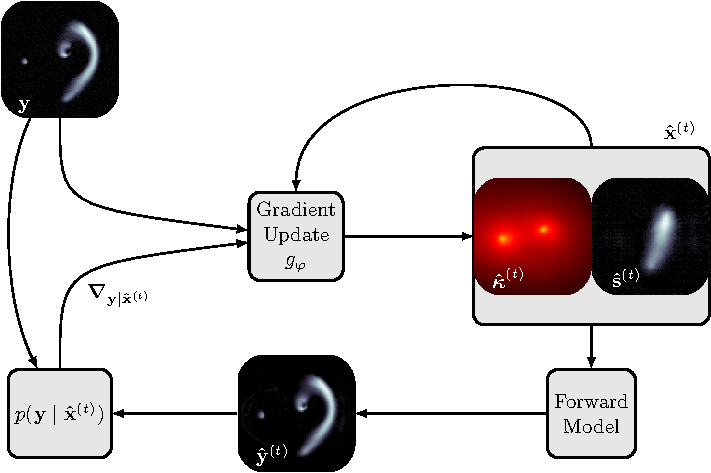
\includegraphics[width=0.7\linewidth]{figures/schematic_rim}
        \caption{Rolled computational graph of the RIM. Dashed arrows represent operations not recorded for BPTT.}
        \label{fig:rolled graph}
\end{figure}


We follow previous works in setting a uniform weight over the time 
steps ($\mathbf{w}^{(t)} = \frac{\mathbf{w}}{T}$). 
The choice of the pixel weights $\mathbf{w}_i$ is informed
by our empirical observations when training the network. Details are reported in appendix \ref{ap:rim training and opt}.

%In figure \ref{fig:unrolled_graph}, we show the unrolled computational graph of the RIM. 
In Figure \ref{fig:rolled graph}, we show the rolled computational graph of the 
RIM. During training of the neural network $g_\varphi$, operations along the solid arrows are being 
recorded for backpropagation through time. 
The recording is stopped along the dashed arrow since these operations 
are part of the forward modelling process and contain no trainable parameters.
%By avoiding the computation of these gradients, training time is reduced and 
%knowledge about the inner workings  
%of a specific likelihood (and forward model) is insulated from the optimization algorithm.
%This is analogous to a common RNN use-case like text generation, where the process responsible 
%for producing the next element in a time series is a black box to the optimization 
%algorithm. 

The gradient of the likelihood is computed using automatic differentiation. Following 
\citep{Modi2021}, we preprocess the gradients using the Adam algorithm \citep{Kingma2014}. 
For clarity, we only illustrate this step in Figure \ref{fig:unet}. 
% \vfill\null

\begin{figure*}[ht!]
        \centering
        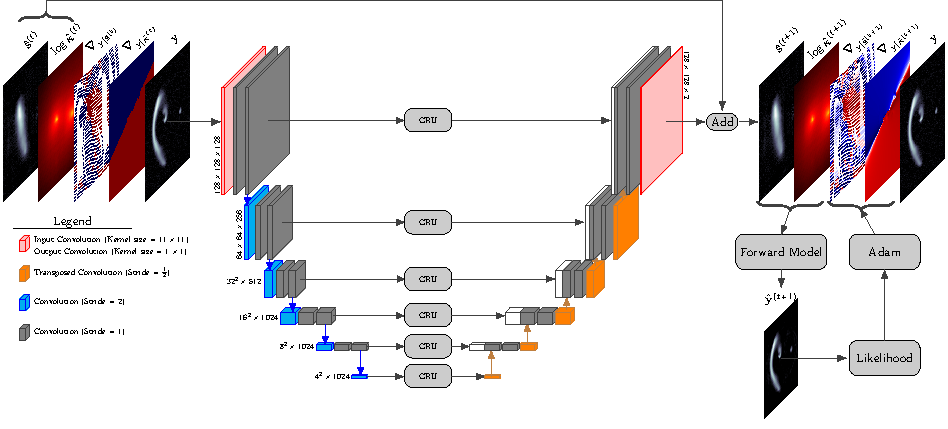
\includegraphics[width=\textwidth]{figures/unet_architecture.pdf}
        \caption{
A single time step of the unrolled computation graph of the RIM.
GRU units are placed in the skip connections to guide the 
reconstruction of the source and convergence. A schematic of the steps to compute 
the likelihood gradients is shown in the bottom right of the figure, including the 
Adam processing step of the likelihood gradient.}
        \label{fig:unet}
\end{figure*}

\subsection{The Neural Network}\label{sec:gradient model}


The neural network architecture is illustrated in Figure \ref{fig:unet}, which shows 
a single time step of the unrolled computation graph of the RIM.
We use a U-net \citep{Ronneberger2015} architecture 
with Gated Recurrent Units \citep[GRU:][]{Cho2014} placed in each skip connection. 

Each GRU cell has its own memory tensor that is updated through time at each iteration of 
equation \ref{eq:RIM}. The shape of a memory tensor is set to match the
feature tensor fed into it from the parent layer in the network graph. 
Instead of learning a compressed representation like in the hourglass
architecture (or autoencoder), the U-net architecture naturally separates the spatial 
frequency components of the signal into its vertical levels. The first level generally encodes 
high frequency features while the lower levels encode low frequency features (due to downsampling of the feature maps). 
Adding an independent memory unit 
at each level preserve this property.

Convolutional layers with a stride of 2 are used for downsampling and 
stride of $\frac{1}{2}$ for upsampling of the feature maps
(identified in blue and orange respectively in figure \ref{fig:unet}). Half-stride convolutions are implemented in practice with the transposed convolution layers from \texttt{Tensorflow} \citep{tensorflow}.
Most layers use a kernel size of $3\times3$, except the first and last layer. 
The first layer has 
larger receptive field ($11\times11$) in order to capture more details in the input tensor. 
The last layer has kernels of size $1\times 1$. 
A $\tanh$ 
activation function is used 
for each convolutional layer, including strided convolutions, except for the output 
layer. The U-net outputs an image tensor with two channels, one dedicated for the update of the source 
and the other for the update of the convergence (see figure \ref{fig:unet}). 
% \vfill\null
%\columnbreak


% Talk about this choice
% Shared memory is important, possibly more than the notion that source and kappa require very different 
% reconstruction procedure (because of different structure etc).

% Choice of model correspond to choosing an inductive bias, or how the function should behave 
% for points in and out of the dataset
% Generalization means the ability to make prediction about the behavior of the function 
% at novel points in the domain of the function.
% In the meta-learning framework, examples are problem instances. Generalization means to transfer 
% knowledge accross problem instances.
% The reuse of the problem structure is known as transfer learning. In the context of meta-learning, 
% this is cast as generalization.


\subsection{Fine-Tuning}\label{sec:fine-tuning}

\subsubsection{Objective function}
Once trained, the RIM produces a baseline (point)
estimate of the parameters $\mathbf{x}$ given a noisy observation $\mathbf{y}$, a PSF and a noise covariance matrix. 
%We note $(\mathbf{y},\Pi,C) \sim \mathcal{T}$.
We now concern ourselves with a strategy to improve 
this estimate. 
This is important 
for observations with high SNR, for which the estimate
must be very accurate to model all the fine features present in the arcs.
The metric for the goodness of fit 
is the reduced chi squared $\chi^2_\nu = \frac{\chi^2}{\nu}$, 
where $\nu$ is the total number of degrees of freedom which here corresponds to 
the total number of pixels in $\mathbf{y}$.
Generally, our goal will be to reach $\chi^2_\nu = 1$, or equivalently $|\chi^2 - \nu| = 0$, 
which suggests that the RIM's estimate has modeled all the signal 
to be recovered from the observations. 
We note that such a problem is exceedingly  
difficult at high SNR. 

We note that we can optimize the log-likelihood directly w.r.t.\ the network weights given an appropriate prior on those weights (to avoid forgetting the implicit priors that have been learned during training, see section \ref{sec:transferlearning}). The new objective function is given by
\begin{equation}\label{eq:MAP} 
        \hat{\varphi}_{\mathrm{MAP}} = \underset{\varphi}{\mathrm{argmax}}\,\, 
        \frac{1}{T}\sum_{t=1}^{T} \log p(\mathbf{y} \mid \mathbf{\hat{x}}^{(t)}) + \log p(\varphi) \, ,
\end{equation} 
where $\varphi$ are the network weights, $\log p(\mathbf{y} \mid \mathbf{\hat{x}}^{(t)})$ is the log-likelihood, and $\log p(\varphi) $ is the log prior over the network weights.
Unlike the loss in equation \eqref{eq:Loss}, this objective function makes no use of labels 
($\mathbf{x}$). 
This allows us to use equation \eqref{eq:MAP} at test time in order to fine-tune the RIM's weights to a specific test example. 

\subsubsection{Transfer Learning}
\label{sec:transferlearning}
We now address the issue of transferring knowledge from the training task defined by the loss function in equation \eqref{eq:Cost}, 
to a test task specific to an observation,  as defined by the loss given in equation \eqref{eq:MAP}.
The reader might refer to reviews on transfer learning \citep{Pan2010,Zhuang2019} 
for a broad overview of the field. The strategy we outline falls within 
the category of inductive transfer learning.

%Despite the second term in Eq \eqref{eq:MAP}, we find 

% Since the data likelihood $p(\mathbf{y} \mid \mathbf{x})$ 
% does not contain \textit{a priori} information 
% about the solution $\hat{\varphi}_{\mathrm{MAP}}$,
% inductive biases must be introduced to make 
% the problem \eqref{eq:MAP} well-posed. Thus, we
% \begin{enumerate}[label=(\subscript{\mathcal{H}}{{\arabic*}})]
%         %\setcounter{enumi}{3}
%         \item \label{prior:initialization} initialize the network parameters with $\varphi_{\mathcal{D}}^{\star}$; 
%         \item \label{prior:early stopping} apply early stopping when a maximum number of steps is reached or 
%                 $\chi^2_\nu \leq 1$;
%         % \item \label{prior:learning rate} use a small learning rate.
% \end{enumerate}
% \ref{prior:early stopping} and \ref{prior:learning rate} encode the assumption 
% that the optimal estimator is to be found \textit{near} the initialization.

\begin{figure}[tb!]
       \centering 
       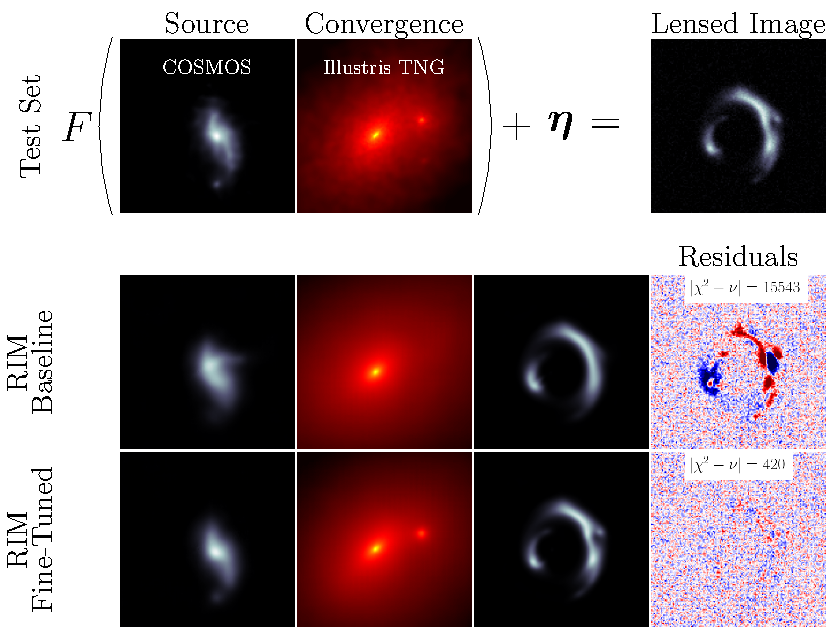
\includegraphics[width=0.8\linewidth]{figures/main_figurev2}
       \caption{Example of a simulated lensed image in the test set that 
exhibits a large deflection in its eastern arc which indicates the presence of a massive object
 --- in this case a dark matter subhalo. The fine-tuning procedure is able to recover 
this subhalo because of its strong signal in the lensed image and reduces the residuals 
to noise level.}
       \label{fig:main figure}
\end{figure}

Optimizing the log-likelihood alone without a prior term over the weights (i.e.~just the first term from the r.h.s.~in \eqref{eq:MAP}) by initializing the weights at $\varphi^\star_\mathcal{D}$ is not strong 
enough to preserve the knowledge learned from the training task. 
This has long been observed in the literature and was coined as the 
catastrophic interference phenomenon in 
connectionist networks \citep{McCloskey1989,Ratcliff1990}.
In summary, a sequential learning problem exhibits catastrophic 
forgetting of old knowledge when confronted with new examples (possibly 
from a different distribution or process), in a manner 
\begin{enumerate}%[label=(\subscript{\mathrm{CF}}{{\arabic*}})]
        \item \label{cf:steps} proportional to the amount of learning;
        \item \label{cf:weights} strongly dependant to the disruption of the parameters
                involved in representing the old knowledge.
\end{enumerate}
While introducing an early stopping condition could 
potentially alleviate the former issue, the latter could still remain a problem.

We therefore follow the work of \citet{Kirkpatrick2016} to define a prior distribution
over $\varphi$ that address this issue
\begin{equation}\label{eq:Prior} 
        \log p(\varphi) \propto -\frac{\lambda}{2}\sum_{j} \mathrm{diag}(\mathcal{I}(\varphi_{\mathcal{D}}^{\star}))_{j} 
        (\varphi_j - [\varphi^{\star}_{\mathcal{D}}]_{j})^{2}\, .
\end{equation} 
where $\mathrm{diag}(\mathcal{I}(\varphi_{\mathcal{D}}^{\star}))$ is the diagonal of the 
Fisher information matrix 
encoding the amount of information that  
some set of gravitational lensing systems from 
the training set, and similar to the observed 
test task, carries about the baseline RIM weights $\varphi_{\mathcal{D}}^{\star}$ 
--- the parameters that minimize the empirical risk (equation \ref{eq:Cost}).
We can also understand this prior using the
Cramér-Rao lower bound 
\citep{Rao1945,Cramer1946}.
%\begin{equation}\label{eq:iCramerRao}
        %\mathrm{Var(\varphi)} \geq \underbrace{(1 + \mathrm{Bias}_{\mathcal{D}}(\varphi))^{2}}_{\lambda_b}\mathcal{I}(\varphi)^{-1}.
%\end{equation} 
The prior can thus be framed as a multivariate 
Gaussian distribution characterised by a diagonal covariance matrix with $\mathrm{diag}(\mathcal{I})$ as its inverse 
and by $\varphi^{\star}_{\mathcal{D}}$ as its first moment. 
Within this view, the  
Lagrange multiplier is 
tuning our estimated uncertainty about the neural network weights 
for the particular task at hand.  
We have included a derivation 
of this term in the appendix \ref{ap:ewc}.

%We define the distribution of examples from $\mathcal{D}$ similar to the test task $\mathcal{T}$ with 
%the surrogate conditional $\tilde{p}(\mathcal{D} \mid \mathcal{T})$. 
Examples are drawn from the set of training examples similar to the test task by sampling the latent space of two variational autoencoders (VAE) that model a distribution over the background sources and the convergence maps respectively (as described in Section \ref{sec:source} and \ref{sec:kappa}) near the baseline prediction of the RIM. In practice, we choose an isotropic Gaussian distribution centered around $\hat{\mathbf{z}}^{(T)}$ --- 
the latent code of the baseline prediction --- as a sampling distribution. While we leave the possibility of improving this choice to future work, it is sufficient for our goals. 
Figure \ref{fig:vae fine-tuning} illustrates examples of what is meant here by \textit{similar}. 

\begin{figure}[t!]
        \centering
        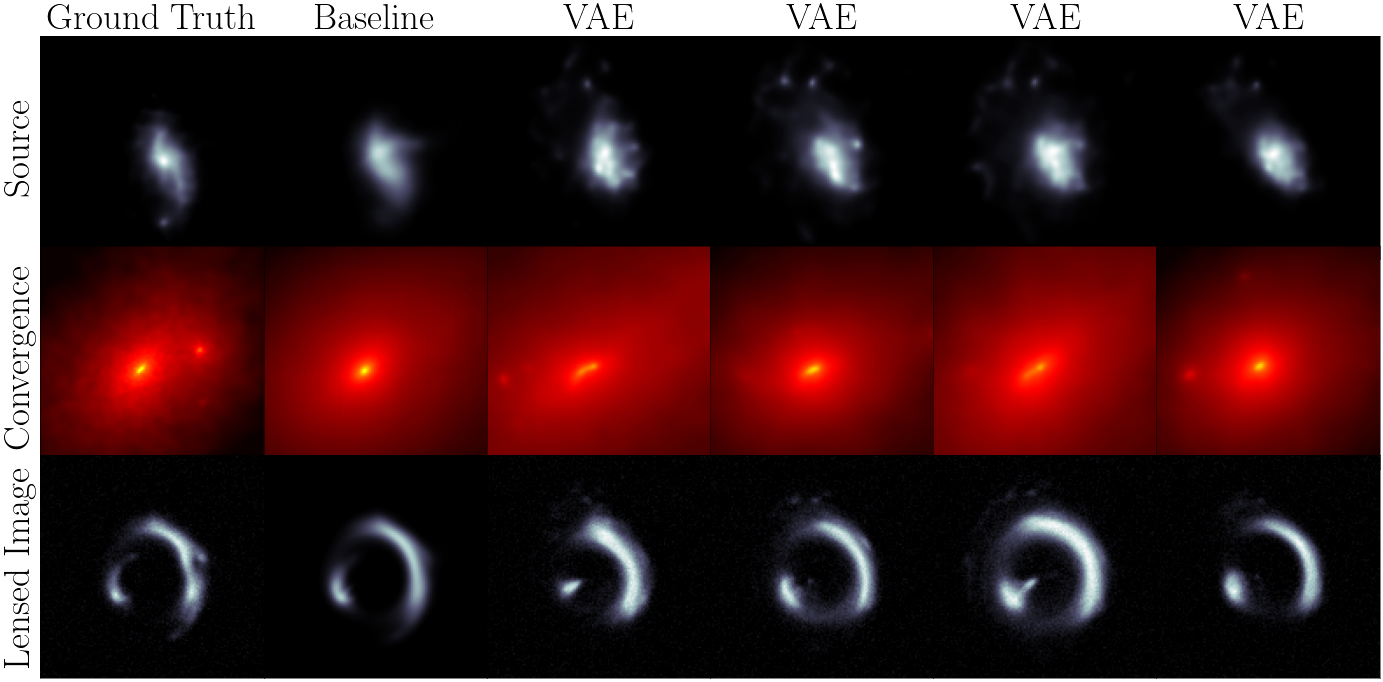
\includegraphics[width=0.8\linewidth]{figures/vae_samples_similar_to_highlight}
        \caption{Examples similar to the test task, also shown in Figure \ref{fig:main figure}. The first column shows the ground truth used to simulate the lensed image. The second column shows the baseline prediction that is then encoded in the latent space of the VAE in order to sample the next 4 columns.
}
        \label{fig:vae fine-tuning}
\end{figure}

%By definition, the Fisher matrix is the 
%expected value of the observed information that 
%the examples carry about $\varphi$. 

%We can, however, make use of theoretical and 
%experimental evidence that overparametrized 
%neural networks exhibits a spectral bias \citep{Rahman2018} 
%toward learning low frequencies first during training. We observe 
%that the baseline model generally 
%provides a coherent prediction ($\gamma(k) = 1$) in the low frequency 
%regime, which is consistent with a spectral bias hypothesis. 
%This suggest a possible approach to ground our method. 
%The MLE-optimal estimator should at least 
%preserve the low frequency features predicted by the baseline. 
%Otherwise, we might suspect that the optimisation procedure 
%has found a degenerate solution that is not consistent with the 
%prior learned by the baseline.

%This also points to interesting strategies that could alleviate 
%overfitting. For instance, freezing the deeper layers of the U-net during 
%fine-tuning might preserve the low frequency features learned during pretraining. 
%This is also suggested as a strong regularization method in \citet{Li2018}. 
%We explore such ideas in the appendice


\section{Data}\label{sec:data}

\subsection{COSMOS}\label{sec:source}
The maps of surface brightness of background sources are taken from the \textit{Hubble Space Telescope} (\textit{HST}) 
Advanced Camera for Surveys Wide Field Channel COSMOS field \citep{Koekemoer2007,Scoville2007},
a $1.64\,\mathrm{deg}^{2}$ contiguous survey acquired in the F814W filter. 
A dataset of magnitude limited ($\mathrm{F814W} < 23.5$) deblended galaxy postage stamps \citep{Leauthaud2007} was compiled as 
part of the GREAT3 challenge \citep{Mandelbaum2014}. The data is 
publicly available \citep{Mandelbaum2012}, and the preprocessing is done through the open-source software 
\texttt{GALSIM} \citep{Rowe2015}. \par

We apply the 
\texttt{marginal} selection criteria (see the \texttt{COSMOSCatalog} class) and impose a flux per image
greater than $50\,\,\mathrm{photons}\,\,\mathrm{cm}^{-2}\,\mathrm{s}^{-1}$. 
This final set has a total of 13\,321 individual images.
Each image is saved as a postage stamp of $158^2$ pixels. 
We then subtract the background from each image, apply a random shift, rotate them by an angle multiple of $90^\circ$, crop them down to $128^{2}$ pixels, and finally normalize them to pixel intensities in the range $[0,1]$. We then train an autoencoder to denoise the galaxy images \citep{Vincent2008,Vincent2010}. More specifically, we use the informational bottleneck principle \citep{Tishby2000} to learn a lossy lower-dimensional representation of the data. For a generic CNN autoencoder, this amount to learning a low-pass frequency filter on the COSMOS dataset. Indeed, CNNs are known to exhibit a spectral bias in their learning phase \citep{Rahaman2018}, which we exploit to our advantage in order to filter pixel noise from the galaxy surface brightness. Furthermore, using an expressive CNN autoencoder produces much less artifacts than a naive implementation of such a low-pass filter --- e.g.\ by masking Fourier modes. 

We split the galaxies into a training set (90\%) and a test set (10\%). 
The augmented training set (${\sim50\,000}$ images) is then used to train a VAE, as described in Section \ref{sec:vae training}, and produce simulated observations to train the RIM.

\begin{figure}[t!]
        \centering
        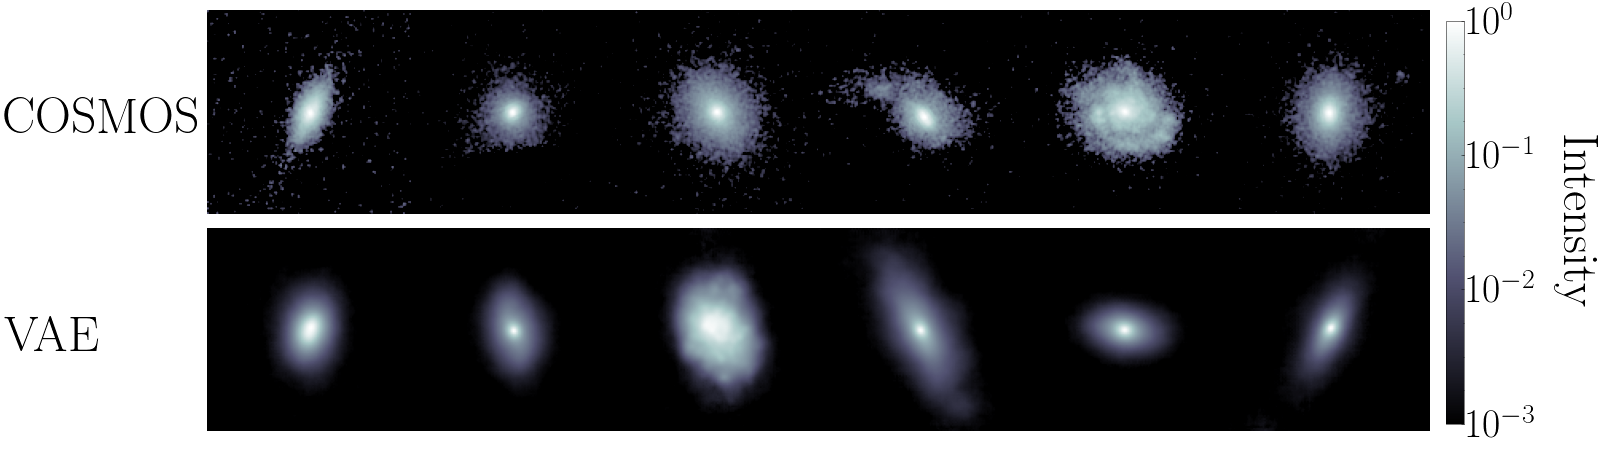
\includegraphics[width=0.8\linewidth]{figures/gal_vae_sample}
        \caption{Examples of COSMOS galaxy images 
                (top row) and VAE generated samples (bottom row) used as labels in $\mathcal{D}$.}
        \label{fig:source}
\end{figure}


\subsection{IllustrisTNG}\label{sec:kappa}
\subsubsection{Smooth Particle Lensing}\label{sec:SPL}
To compute convergence maps from an N-body simulation, 
we use Kernel Density Estimation to produce smooth densities on a regular grid from discrete simulation particles.
This reduces the particle noise affecting all 
important lensing quantities. At the same time, the choice of the kernel size 
is important to preserve substructures in the 
lens that we might potentially be interested in. Following \citet{Aubert2007,Rau2013}, we use Gaussian smoothing with an adaptive kernel size determined by the distance of the 64\textsuperscript{th} nearest neighbours of 
a given particle $D_{64,i}$. 
\begin{equation}\label{eq:Ksmooth}
\begin{aligned}
    \kappa(\mathbf{x}) &= \frac{1}{\Sigma_{\mathrm{crit}}} \sum_{i=1}^{N_{\mathrm{part}}}
        \frac{m_i}{2 \pi \hat{\ell}^2_i} 
        \exp \left(-\frac{1}{2} \frac{(\mathbf{x} - \mathbf{x}_i)^2}{\hat{\ell}_i^2}  \right) \\
    \hat{\ell}_i &= \sqrt{\frac{103}{1024}}D_{64,i}.
\end{aligned}
\end{equation}
The nearest neighbours are found by fitting a k-d tree ---  implemented in 
\texttt{scikit-learn} \citep{scikit-learn} --- 
to the $N_{\mathrm{part}}$  particles 
in a cylinder centered on the centre of mass of the halo of interest.
The critical surface density is defined as
\begin{equation}\label{eq:Scrit}
\Sigma_{\mathrm{crit}} = \frac{4 \pi G}{c^ 2} \frac{D_\ell D_{\ell s}}{D_s},
\end{equation}
where $D_\ell$, $D_s$ and $D_{\ell s}$ are angular diameter distances to the lens, source and between the lens and the source respectively, 
$G$ is the gravitational constant, and $c$ the speed of light.

\subsubsection{Preprocessing}
The projected surface density maps (convergence) of lensing galaxies 
were made using the redshift $z=0$ snapshot  
of the IllustrisTNG-100 simulation \citep{Nelson2018} 
in order to produce physically realistic realizations of density maps containing dark and baryonic matter.
We selected 1604 halos with the criteria that they have a total
dark matter mass of at least $9\times10^{11} M_{\odot}$. We then collected all 
dark matter, gas, stars and black holes particles from the data in the vicinity of the halo. We then create a smooth projected surface density map as prescribed in section \ref{sec:SPL}.

\begin{figure}[t!]
        \centering
        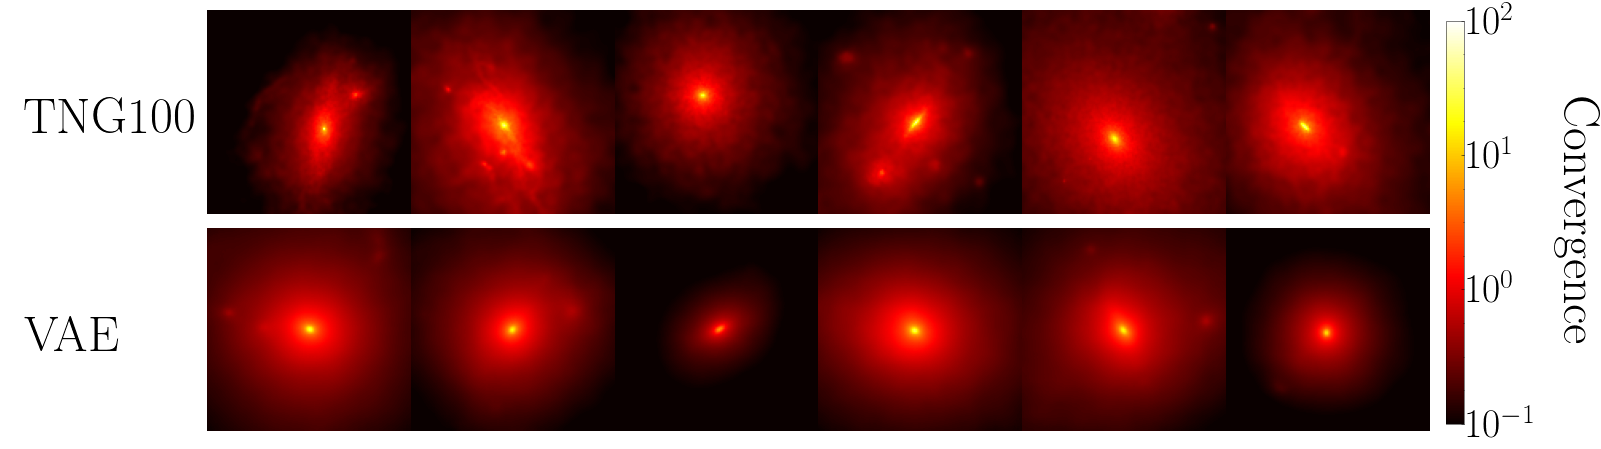
\includegraphics[width=0.8\linewidth]{figures/kap_vae_sample}
        \caption{Examples of smoothed Illustris TNG100 convergence map (top row) 
        and VAE generated samples (bottom row) used as labels in $\mathcal{D}$.}
        \label{fig:kappa}
\end{figure}

We adopt the $\Lambda$CDM cosmology from 
\citet{PlanckCollaboration2018} with $h=0.68$ to compute 
angular diameter distances. We also fix the 
source redshift to $z_s=1.5$ and the deflector redshift to $z_\ell=0.5$. 
We note that changing the redshifts or the cosmology 
only amount in a rescaling of the $\kappa$ map by a global scalar. Thus, this choice does not change the generality of our method.
The smoothed density maps from equation \eqref{eq:Ksmooth} are 
rendered into a regular grid of $188^2$ pixels with a comoving field of view of $105\,\,\mathrm{kpc}/h$. 
To avoid edge effects in the pixelated maps, 
we include particles outside of the field of view in the sum of equation \eqref{eq:Ksmooth}.
\par
Before applying augmentation or considering different projections, our dataset of halos is split into a 
training set (90\%) and a test set (10\%), in order to make sure that the test set consists only 
of convergence maps unseen by the RIM during training.
We take 3 different projections ($xy$, $xz$ and $yz$) of each 3D particle 
distribution, which amounts to a dataset with a total of $4\,812$ individual convergence maps. 
Random rotations by an angle multiple of $90^{\circ}$ and random shifts to the pixel coordinates 
are applied to each image. The $\kappa$ maps are then rescaled by a random factor to change their 
estimated Einstein radius to the range 
$[0.5,\,2.5]$ arcseconds.
The Einstein radius is defined as
\begin{equation}\label{eq:ThetaE}
        \theta_E = \sqrt{\frac{4GM(\theta_E)}{c^ 2} \frac{D_{\ell s}}{D_\ell D_s}}
\end{equation} 
where $M(\theta_E)$ is the mass enclosed inside the Einstein radius. In practice, we estimate this quantity 
by summing over the mass of pixels with a value greater than the critical density ($\kappa > 1$). 
For data augmentation purposes, this procedure gives a good enough estimate of the lensed image separation resulting from a given $\kappa$ map. 
We test multiple scaling factors for each $\kappa$ map, then uniformly sample between those that produce an estimated 
Einstein radius within the 
desired range. This step is used to remove any bias in the Einstein radius that might come from the mass function 
of the simulation.

The final maps are cropped down to $128^2$ pixels.
Placed at a redshift $z_\ell=0.5$, a $\kappa$ map will thus span an angular field of view of $7.69''$ with 
a resolution similar to \textit{HST}. 
%This field of view is wide enough to cover a typical gravitational 
%lens observed in the sky, which partly justify our choice for the comoving field of view earlier. 
With these augmentation procedures, a total of $50\,000$ maps are created from the training split
to train a VAE, as described in Section \ref{sec:vae training}, and produce simulated observations to train the RIM. 

\subsection{Simulated Observations}\label{sec:simulated observation}
Having defined a source map and a convergence map, we apply the ray tracing simulation 
described in section \ref{sec:forward model} to produce a lensed image. 

For each lensed image, a Gaussian PSF is 
created with a full width at half maximum (FWHM) 
randomly generated from a truncated normal distribution.
The support of the distribution is truncated below by the 
angular size of a single pixel and above by the angular size of 4 pixels. 
White noise with a standard deviation randomly generated from a truncated normal distribution 
is then added to the convolved lensed image to simulate noisy observations. These noise realizations result in SNRs between 
$10$ and $1000$. For simplicity, we define $\mathrm{SNR} = \frac{1}{\sigma}$. 
This definition is equivalent to the peak signal-to-noise ratio. 

%We set the observed image field of view to match with the convergence field view ($7.69''$). 
%We choose the background field of view to be $3''$.
To ensure that the images are representative of strongly lensed source, we require a minimum flux magnification of 3. We
also make sure that most pixel coordinates in the image plane are mapped inside the 
source coordinate system through the lens equation \eqref{eq:LensEquation}. 

\begin{table}[htb!]
\centering
\caption{Physical model parameters.}
\label{tab:phys}
\begin{tabular}{ccc}
        Parameter &  Distribution/Value \\
        \hline \hline
        Lens redshift $z_\ell$ & $0.5$ \\
        Source redshift $z_s$ & $1.5$ \\
        Field of view ('') & $7.69$ \\
        Source field of view ('') & $3$ \\
        PSF FWHM ('') & $\mathcal{TN}(0.06,\, 0.3;\, 0.08,\, 0.05)$
        \footnote{We defined the parameters of the truncated normal in the order $\mathcal{TN}(a,\, b;\, \mu,\, \sigma)$, where $[a,\, b]$ defines the support of the distribution.} \\
        Noise amplitude $\sigma$ & $\mathcal{TN}(0.001,\, 0.1;\, 0.01,\,0.03)$\\
        \hline
\end{tabular}
\end{table}

In total, $400\,000$ training observations are simulated from random pairs of COSMOS sources 
and IllustrisTNG convergence maps in order to train the RIM. 
An additional $200\,000$ observations are created from pairs 
of COSMOS sources and pixelated SIE convergence maps. 
The parameters for these $\kappa$ maps are listed in table \ref{tab:sie}. 
% We expect some lensing configurations like doubly imaged systems to poorly constrain the inner structure of the 
% mass distribution. 
% Building an inference pipeline with strong constraints (other than the lensed image) on the 
% slope of the profile goes beyond the scope of this work. 
% As such, imposing an implicit prior for the slope through 
% the dataset is sufficient for our goal. 
% It is also motivated by the \textit{bulge-halo conspiracy} --- 
% the observation that most lensing configurations observed in the sky can be explained 
% to a first order approximation by 
% an average slope consistent with an isothermal profile \citep{Auger2010,Dutton2014}.

\begin{table}[htb!]
\centering
\caption{SIE parameters.}
\label{tab:sie}
\begin{tabular}{ccc}
        Parameter &  Distribution \\
        \hline \hline
         Radial shift ('') & $\mathcal{U}(0, 0.1)$ \\
        Azimutal shift & $\mathcal{U}(0, 2\pi)$ \\
        Orientation & $\mathcal{U}(0, \pi)$ \\
        $\theta_E$ ('') & $\mathcal{U}(0.5, 2.5)$ \\
        Ellipticity & $\mathcal{U}(0, 0.6)$ \\
        \hline
\end{tabular}
\end{table}


We generate $1\,600\,000$ simulated observations from the VAE 
background sources and convergence maps as part of the training set. We apply some validation checks to each example in order to avoid configurations like a single image of the background source or an Einstein ring cropped by the field of view.
% In principle, we could generate as many simulated observations as needed from the VAE. 
% However, having a set of finite, fixed size lets us apply some validation checks to each 
% example in order to avoid configurations like a
% single image of the background 
% source or an Einstein ring cropped by the field of view.




\section{Training}\label{sec:training}

\subsection{VAE}\label{sec:vae training}
Here, we describe the training of two VAEs that are used to produce density maps and images of unlensed background galaxies to train and test our inference model. For an introduction to VAEs we refer the reader to \citet{Kingma2019}.

As mentioned in \citet{Kingma2019}, direct optimisation 
of the ELBO loss can prove difficult because the reconstruction term $\log p_\theta (\mathbf{x} \mid \mathbf{z})$ 
is relatively weak compared to the Kullback Leibler (KL) divergence term. To alleviate this issue, 
we follow the work of \citet{Bowman2015} and \citet{Sonderby2016} in setting a warm-up 
schedule for the KL term, starting from $\beta=0.1$ up to $\beta_{\mathrm{max}}$. 

Usually, 
$\beta_{\mathrm{max}} = 1$ is considered optimal since it matches the original ELBO  
objective derived by \citet{Kingma2013}. 
However, we are more interested in the 
sharpness of our samples and accurate inference around small regions of the latent 
space for fine-tuning. Thus, setting $\beta_{\mathrm{max}} < 1$ allows us to increase 
the size of the information bottleneck (i.e.~latent space) of the VAE 
and improve the reconstruction cost of the model. 
This is a variant of the $\beta$-VAE \citep{Higgins2017}, where $\beta > 1$ was found 
to improve disentangling of the latent space \citep{Burgess2018}. 

The value for $\beta_\mathrm{max}$ and the steepness of the schedule 
are grid searched alongside the architecture for the VAE. 
These values are found in practice by 
manually looking at the quality of generated samples for different VAE 
hyperparameters. A similar method is explored and formalized in the 
InfoVAE framework \citep{Zhao2017}.


A notable element of the VAE architecture is the use of a fully connected
layer to reshape the features of the convolutional layer into the chosen 
latent space dimension. Following the work of \citet{Lanusse2021}, we introduce 
an $\ell_{2}$ penalty between the input and output of the bottleneck 
dense layers to encourage an identity mapping. This regularisation 
term is slowly removed during training.


\subsection{RIM}\label{sec:rimtraining}

The architecture of the neural network was grid searched on 
a smaller dataset ($\lesssim 10\,000$ examples) 
in order to quickly identify a small set
of valid hyperparameters. Then, the best hyperparameters were 
identified using a two-stage training process on the training dataset. 
In the first stage, we trained 24 different architectures from this small hyperparameter set for approximately 4 days (wall time using a single Nvidia A100 GPU). 
Different architectures would have a training time much longer than others, and this 
was factored in the architecture selection process. For example, adding more time steps ($T$) to the recurrent relation \eqref{eq:RIM} 
would yield better generalisation on the test set, but this 
would come at great costs to training time until convergence. 

Following this first stage, 4 architectures were deemed efficient enough 
to be trained for an additional 6 days. 
We only report the results for the best architectures out of these 4.
%We report the hyperparameters for 
%the best architecture after this second stage of training in table \ref{tab:baseline hparams}.

Each reconstruction is performed by fine-tuning the baseline model 
on a test task composed of an observation vector, a PSF, and a noise covariance.
In practice, fine-tuning predictions on the test set of $3\,000$ examples can be accomplished in parallel so as to be done in at most a few days by spreading the computation on $\sim 10$ Nvidia A100 GPUs. Each reconstruction uses at most 2000 steps, correspondling to approximately $20$ minutes (wall-time) per reconstruction. Early stopping is applied when the $\chi^2$ reaches noise level. The hyperparameters for this procedure are reported in Table \ref{tab:fine-tuning hparams}.


\begin{table}[H]
        \centering
        \caption{Hyperparameters for fine-tuning the RIM.}
        \label{tab:fine-tuning hparams}
        \begin{tabular}{cc}
                Parameter & Value \\\hline\hline
                Optimizer & RMSProp \\
                Learning rate & $10^{-6}$\\
                Maximum number of steps & $2\,000$\\
                $\lambda$ & $2\times 10^{5}$\\
                $\ell_2$ & 0 \\
                Number of samples from VAE & 200 \\
                Latent space distribution & $\mathcal{N}(\mathbf{z}^{(T)}, \sigma=0.3)$
                \footnote{$\mathbf{z}^{(T)}$ is the latent code of the RIM baseline source or convergence.}\\
                \hline
        \end{tabular}
\end{table}



\begin{figure}[H]
        \centering
        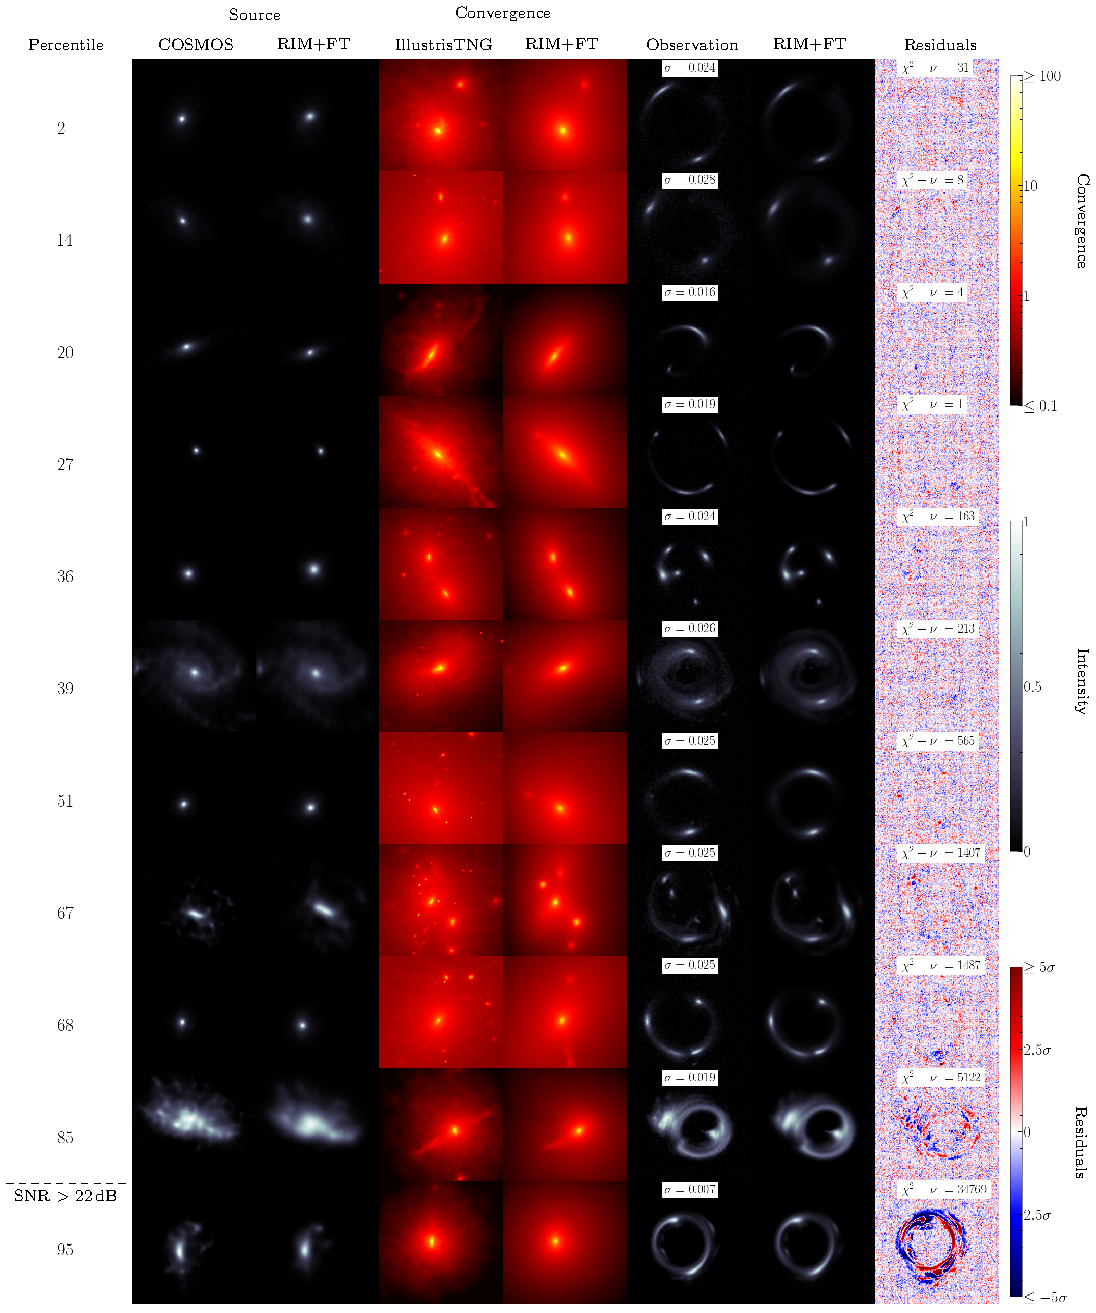
\includegraphics[width=\linewidth]{figures/main_result}
        \caption{
                Sample of the fine-tuned RIM reconstructions 
                on a test set of 3000 examples. 
                Examples are ordered from the best $\chi^2$ (top) to the worst (bottom). 
                The percentile rank of each example is in the leftmost column. 
                The last example 
        shown has SNR above the threshold defined in Figure \ref{fig:chi squared vs noise}.}
        \label{fig:main result}
        %\vspace{-1.5pt} % fix
\end{figure}

\begin{figure}[H]
        \centering
        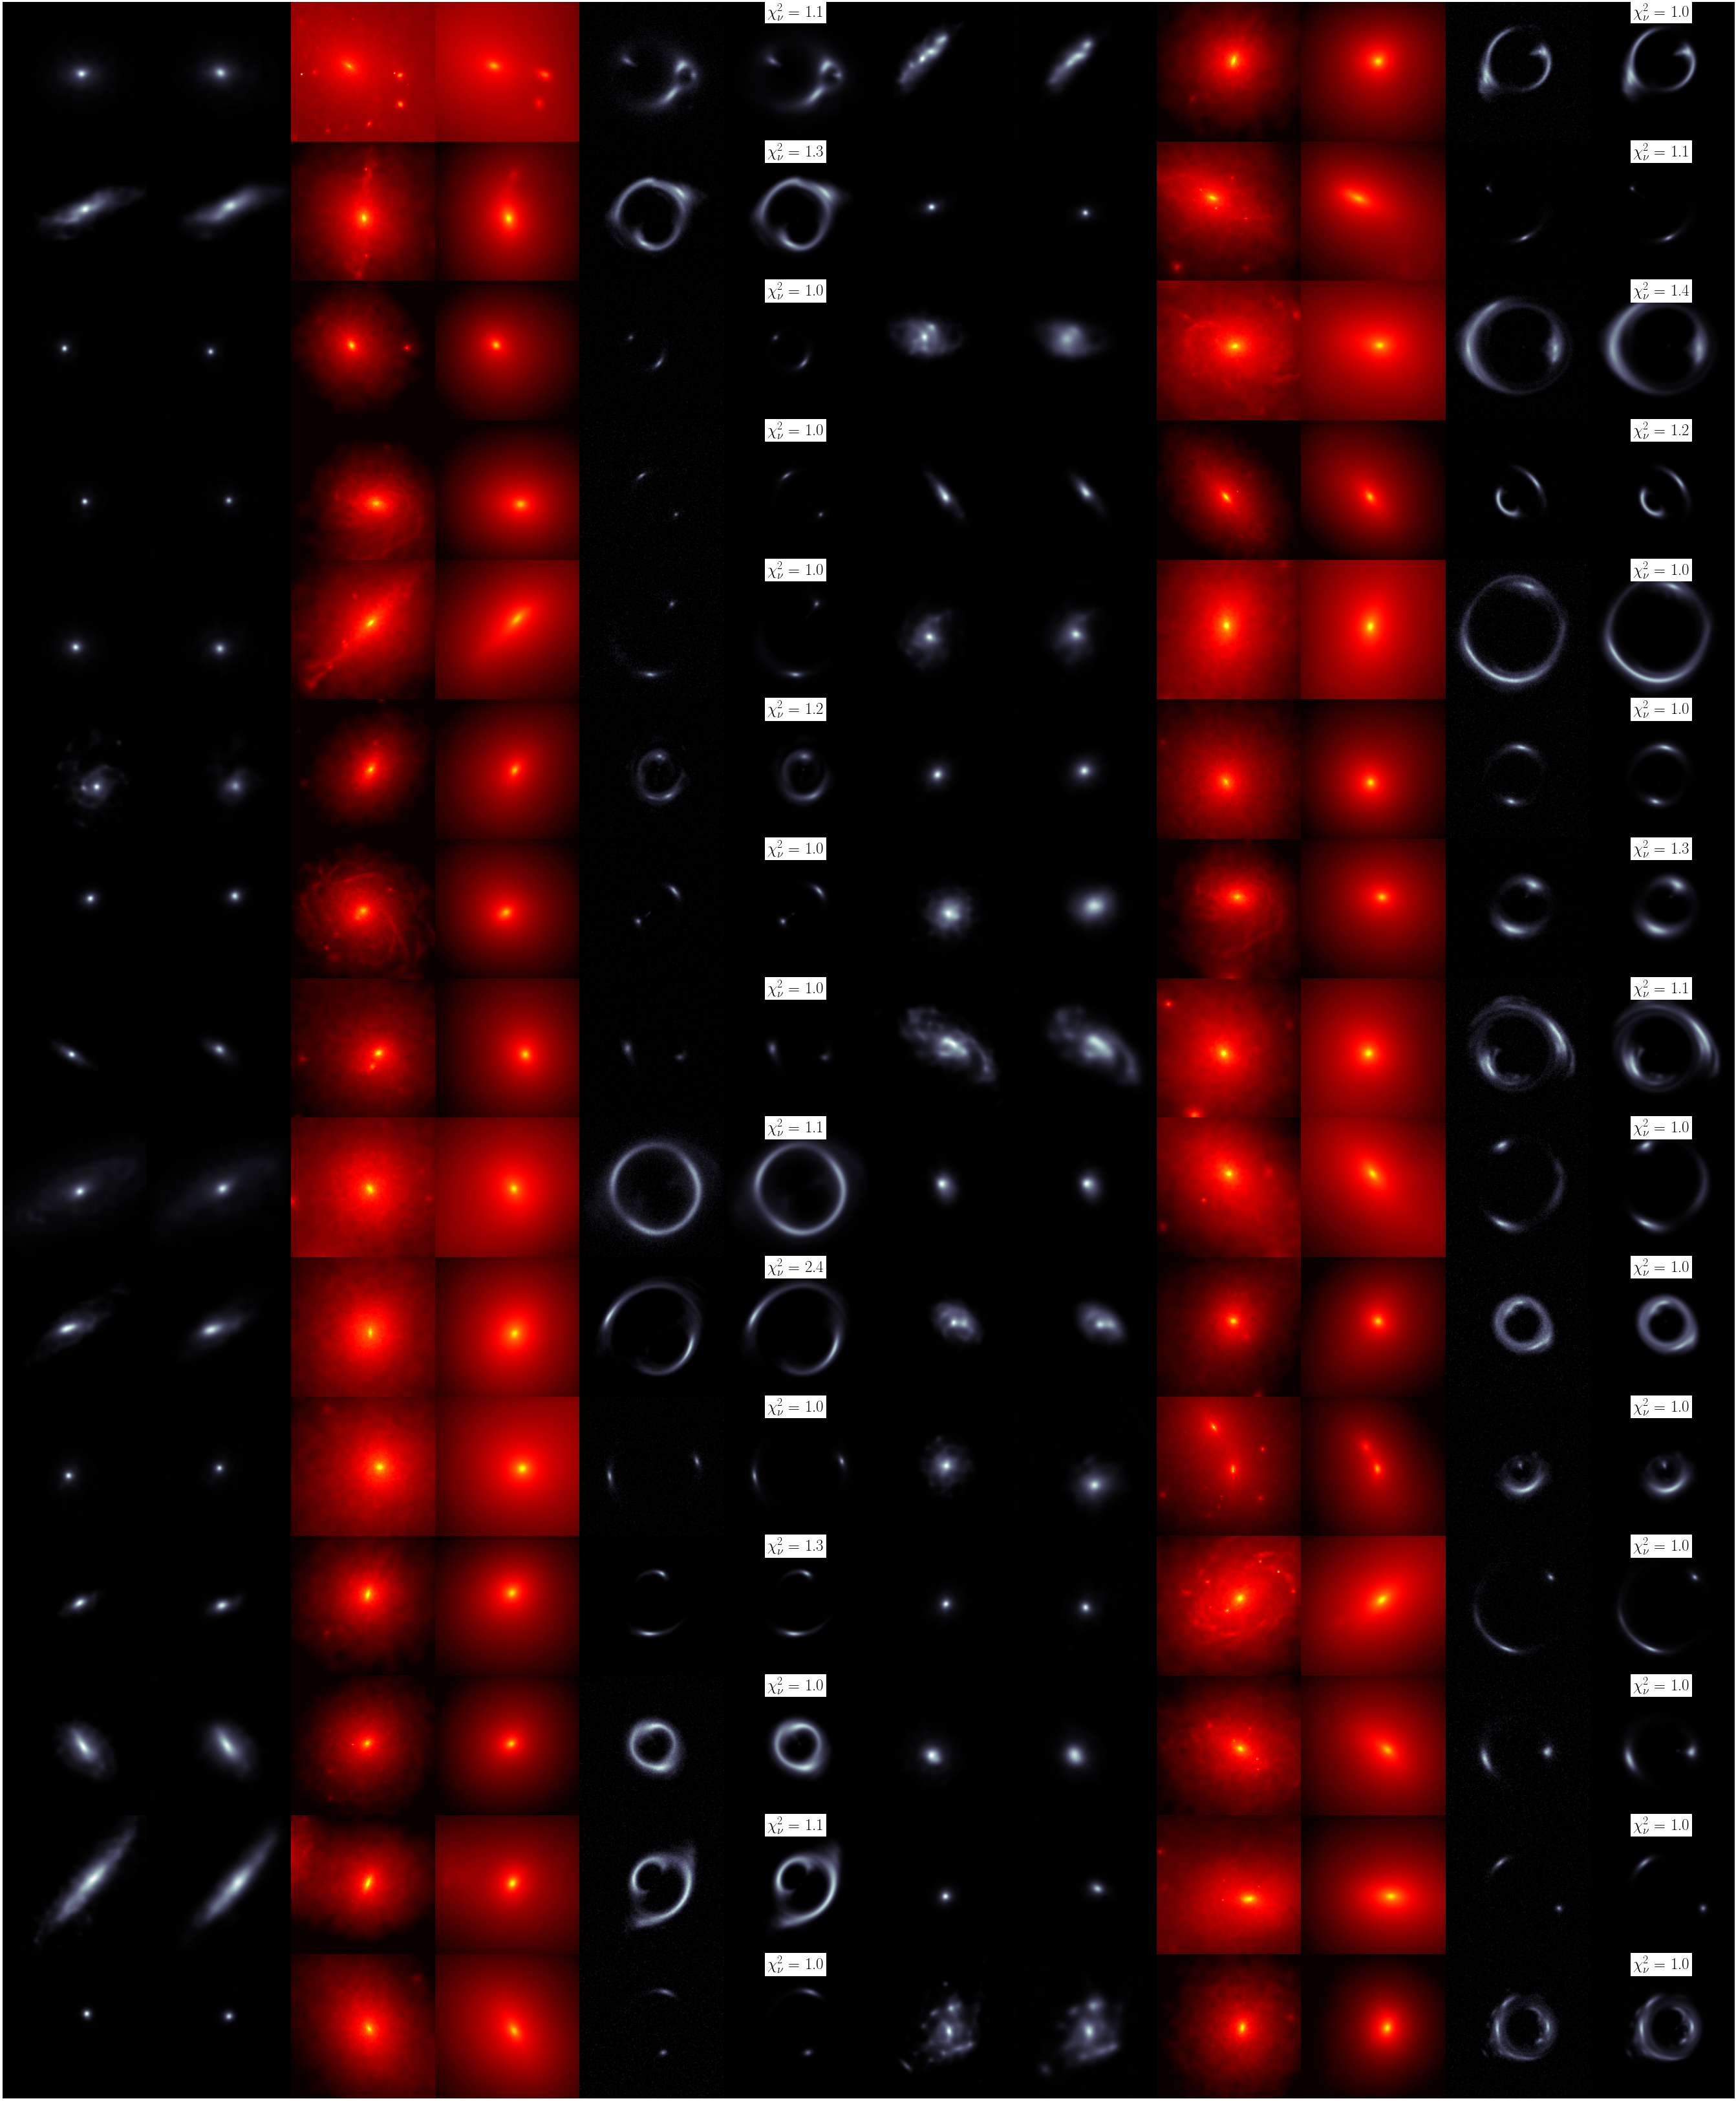
\includegraphics[width=\linewidth]{figures/test_set_no_cherry_pick}
        \caption{
                30 reconstructions taken at random from the test set of 3000 examples simulated from COSMOS 
                and IllustrisTNG data at high SNR.
                The colorscale are the same as in Figure \ref{fig:main result}.}
        \label{fig:random sample}
	\vspace{-1.5pt} % fix
\end{figure}


\section{Results}\label{sec:results}

In this section, we present the performance of our model 
on the held out test set. A sample of 3000 reconstruction 
problems is generated from the held-out \textit{HST} and IllustrisTNG data 
with noise levels and PSFs similar to the training set.

\subsection{Goodness of Fit}
Figure \ref{fig:main result} shows a sample of reconstructions for high SNR data with a wide range of lensing configurations from the test set.
We select examples representative of all levels of reconstruction performance (covering the entire range of goodness of fit) for data with  complex structures in their convergence map to showcase the expressivity of the approach. 
We also show a randomly selected sample from the test set in Figure \ref{fig:random sample}.

\begin{table}[H]
    \centering
    \caption{$\log_{10}$-normal moments of the loss on the test set}
    \label{tab:loss}
    \begin{tabular}{ccc}
        \hline
          Model  & $\mu(\log \mathcal{L}_\varphi)$ & $\sigma(\log \mathcal{L}_\varphi)$ \\
        \hline \hline
        Baseline ($\varphi_{\mathcal{D}}^\star)$ &  -1.96 & 0.36 \\
        Fine-tuned ($\hat{\varphi}_{\mathrm{MAP}}$) & -2.02 & 0.37 \\\hline
    \end{tabular}
\end{table}


\begin{figure}[H]
        \centering
        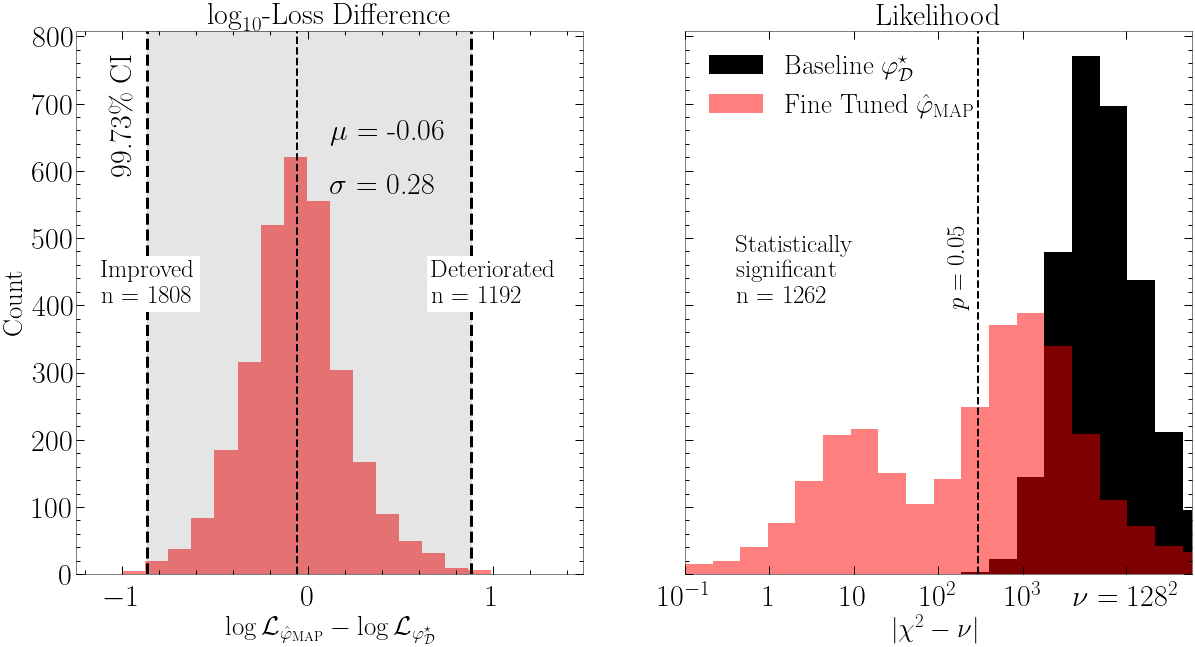
\includegraphics[width=0.8\textwidth]{figures/loss_and_likelihood}
        \caption{Distribution of the goodness of fit for the baseline and fine-tuned network (right panel), as well as log-loss difference between the two network for a given example in the test set (left panel).
}
        \label{fig:loss and chi squared}
\end{figure}


Figure \ref{fig:loss and chi squared} shows a comparison between 
the goodness of fit of the baseline model and the fine-tuned prediction. 
Since we empirically observe that the distribution of the loss on the test set (and the training set) follows a log-normal distribution, we find that it is more informative to look at the $\log$-loss 
distribution to extract information about the fine-tuning procedure. 
The left panel of Figure \ref{fig:loss and chi squared} 
shows the distribution of the log-loss difference between the fine-tuned prediction and the baseline model. This distribution shows that the fine-tuning procedure loss is constrained within $\sim 1$ order of magnitude of the original loss with a probability $>99.73\,\%$. We find that the log-loss difference has a scatter of $\sigma = 0.28$, which is smaller than the scatter of the baseline log-loss over the entire test set $\sigma(\log \mathcal{L}_{\varphi^\star_{\mathcal{D}}}) = 0.36$ reported in Table \ref{tab:loss}.
We note that the loss is not optimized during fine-tuning, still we notice that the fine-tuning procedure does not significantly deteriorate or improve the loss of the baseline prediction on average. We report the first 2 moments of the loss log-normal distribution for the baseline and the fine-tuned reconstructions in Table \ref{tab:loss} in order to explicitly compare them. As can be seen in this table, there is no significant difference between the two distributions. This statement can be proven for the measured mean values --- $\mu(\log \mathcal{L}_{\hat{\varphi}_{\mathrm{MAP}}}) = \mu(\log \mathcal{L}_{\varphi^{\star}_{\mathcal{D}}}) $ --- using the two-sided normal p-value test \citep{Casella2001}, which we find satisfy the null hypothesis with $p=0.87288$ ($Z = -0.16$). All those observations support our claim that EWC regularisation preserves the prior learned during pretraining, or at least that it preserves the surrogate measures of the prior we reported. 

\begin{figure}[H]
        \centering
        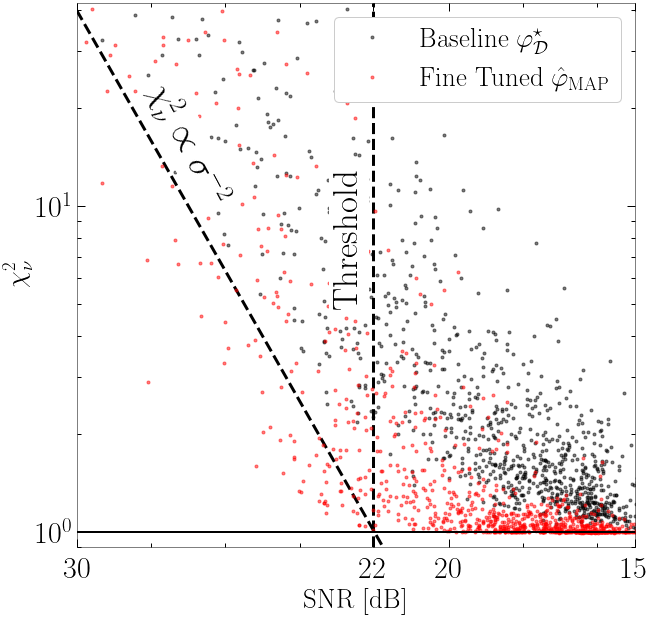
\includegraphics[width=0.6\linewidth]{figures/chisq_vs_noise_ewc}
        \caption{Goodness of fit as a function of SNR shows a threshold 
        behavior where our method reaches its limit.}
        \label{fig:chi squared vs noise}
\end{figure}



The right panel of Figure \ref{fig:loss and chi squared} shows the distribution of  $\chi^2$ for the test set before and after the fine-tuning procedure and the theoretical $\chi^2$ distribution corresponding to $\nu=128^2$ degrees of freedom.
We observe that the fine-tuning procedure significantly improves our $\chi2$, bringing their distribution closer to that of the expected $\chi^2$ distribution (black curve). However, the improved distribution is still far from the theoretical expectation, implying that there are statistically significant residuals in a subset of the reconstructions.

In figure \ref{fig:chi squared vs noise}, we explore how the goodness of fit of the fine-tuned RIM changes as a function of SNR over the examples in the test set. Two behaviors can be identified. For SNR below a certain threshold, the goodness of fit 
of the fine-tuned model is essentially flat, with a certain scatter, around the noise level. This scatter increases as a function of SNR, which reflects the fact that above a certain SNR threshold (vertical dashed line in Figure \ref{fig:chi squared vs noise}), our reconstructions are dominated by systematics in the inference algorithm.
For SNR above the threshold, 
the goodness of fit follows the trend $\chi^2 \propto \sigma^{-2}$ (the solid line in Figure \ref{fig:chi squared vs noise}), which 
means the reconstructions have stopped improving on par with the SNR.

This behavior is exhibited in a few examples of reconstructions taken from the test set in Figure \ref{fig:increasing SNR}, where we ordered reconstructions with increasing SNR from top to bottom and plotted the surface brightness and foreground densities in log scale. As can been seen, errors in reconstructed parameters remain of the same order of magnitude as SNR is increased from $\sim$220 to 500, implying that above this SNR threshold, the reconstructions are dominated by systematics. 

\begin{figure}[H]
        \centering
        \tikzset{font={\fontsize{8pt}{12}\selectfont}}
        \begin{tikzpicture}
                \node at (0, 0) {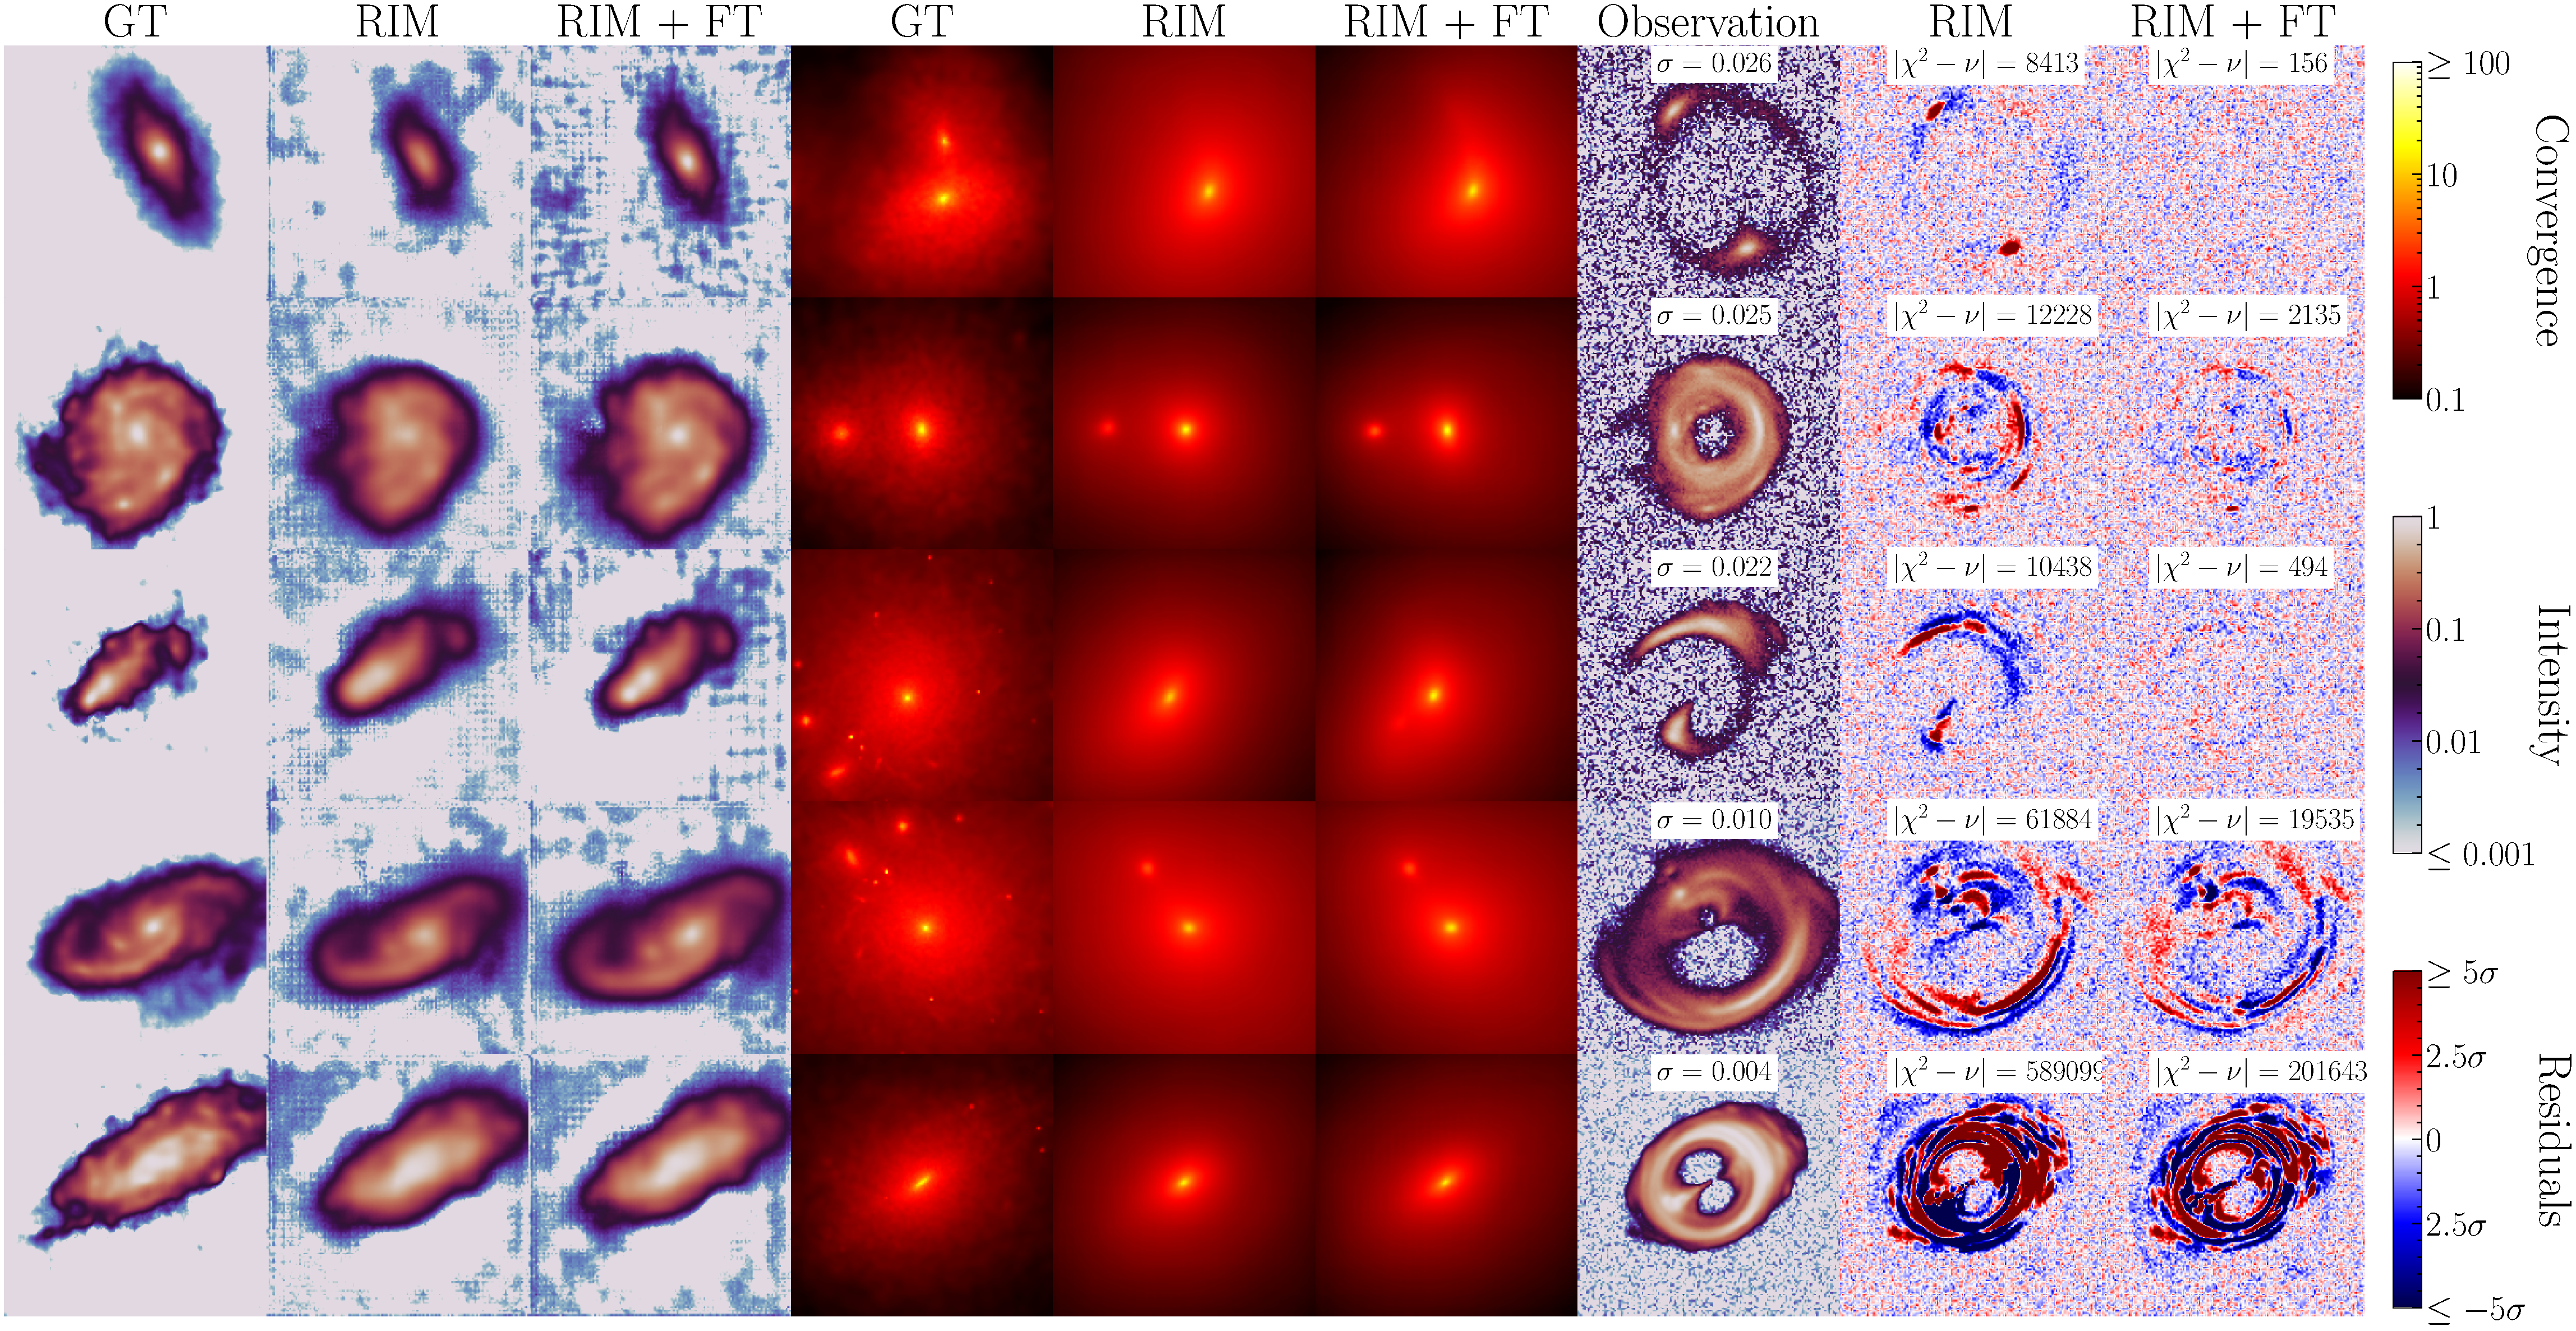
\includegraphics[width=\linewidth]{figures/rim_map_wrt_snr.pdf}};
                \draw[-latex] (-8.5, 3.5) -- (-8.5, -3.5) node[midway, above, rotate=90] {Increasing SNR};
                \node at (-5.5, 4.5) {\strut Source};
                \node at (-0.75, 4.5) {\strut Convergence};
                \node at (5, 4.5) {\strut Residuals};
        \end{tikzpicture}
        \caption{
        Comparison between baseline (RIM) and fine-tuned (RIM+FT) reconstructions for gravitational lensing systems from the test set (GT).
        From top to bottom, we increase SNR. 
        }
        \label{fig:increasing SNR}
\end{figure}
%\vfill\null 

\subsection{Quality of the Reconstructions}\label{sec:quality of reconstructions}

\begin{figure}[H]
        \centering
        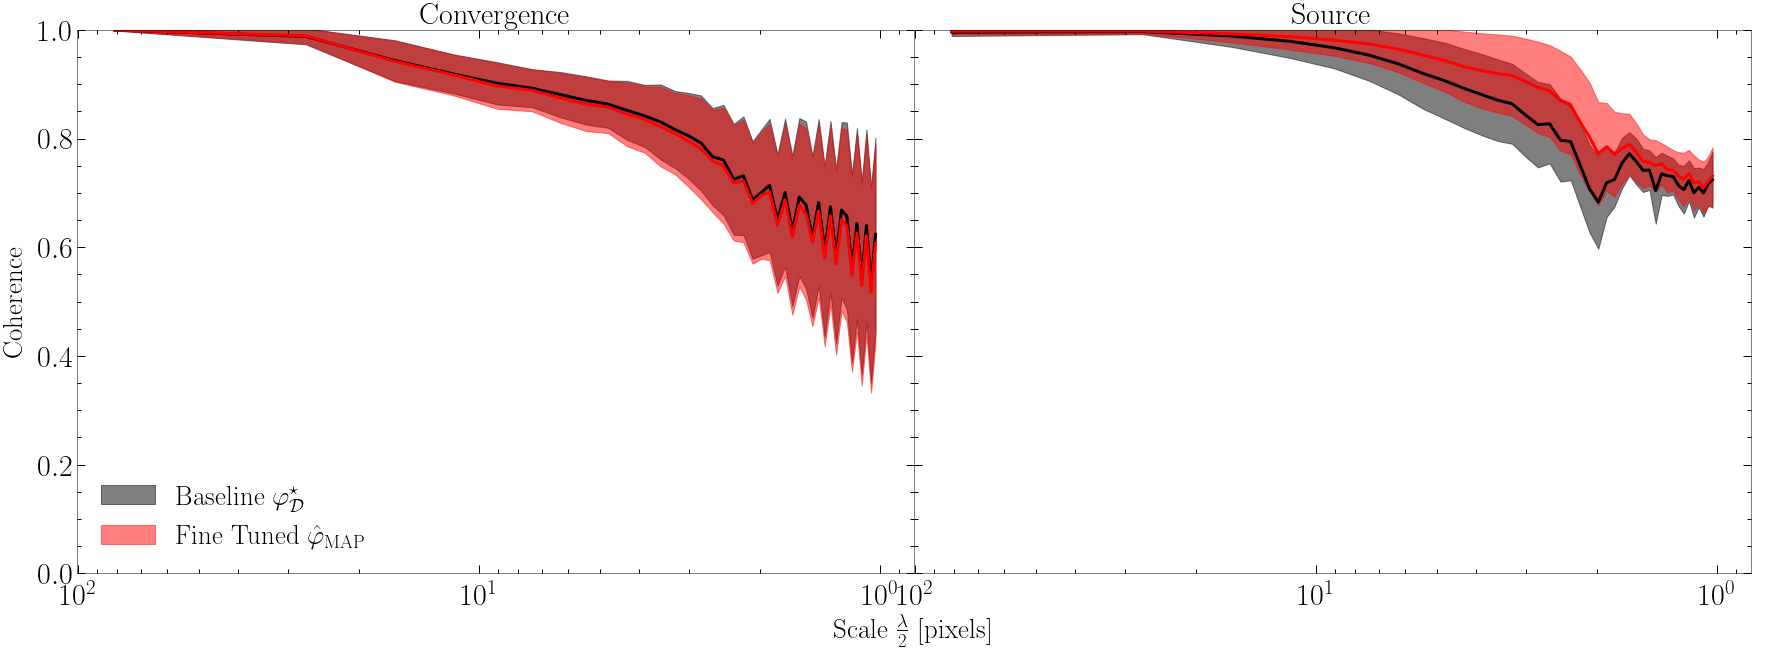
\includegraphics[width=0.8\linewidth]{figures/coherence_spectrum}
        \caption{Statistics of the coherence spectrum on the test set. The solid line is the average 
        coherence. The transparent region is the $68\%$ confidence interval. The fine-tuning 
        procedure yields a noticeable improvement on the coherence of the source at all frequencies.}
        \label{fig:coherence}
\end{figure}


In addition to a visual inspection of the reconstructed sources 
and convergences, we compute 
the coherence spectrum to quantitatively assess the quality of the reconstructions
\begin{equation}\label{eq:coherence} 
        \gamma(k) = \frac{P_{12}(k)}{\sqrt{P_{11}(k) P_{22}(k)}} \, .
\end{equation}

Here, $P_{ij}(k)$ is the cross power spectrum of images $i$ and $j$ at 
the wavenumber $k$. Figure \ref{fig:coherence} shows the mean value and the $68\%$ inclusion interval of $\gamma(k)$ 
for the convergence and source maps in a test set of 3000 examples. 
The fine-tuning 
procedure, shown in red, is able to significantly improve the coherence of the baseline background 
source, shown in black, at all scales. 
The coherence spectrum of the convergence sees a slight improvement due to the fine-tuning procedure.
Still, we note that many examples in the dataset exhibit significant 
improvement, which we illustrate in Figure \ref{fig:main figure}.
%In this case, the observed lensed image exhibits a large deflection in 
%its eastern arc which indicates the presence of a massive object --- in this 
%case a dark matter subhalo. The fine-tuning procedure is able to recover 
%this subhalo because of its strong signal in the lensed image.


\section{Conclusion}\label{sec:conclusion}
The results obtained here demonstrate the effectiveness of machine learning methods, specifically a recurrent inference machine, for inferring pixelated maps of the distribution of mass in lensing galaxies and the distribution of surface brightness in the background galaxies. Since this is a heavily under-constrained problem, stringent priors are needed to avoid overfitting the data, a task that has traditionally been difficult to accomplish with traditional statistical models \citep[e.g., ][]{Saha1997}. The model proposed here can implicitly learn these priors from a set of training data. 

The fine-tuning step that we propose in this work is a general procedure (i.e.\ not specific to our model or problem), which enables us to exploit a diagonal second-order Laplace approximation of the implicit prior learned by a baseline estimator during pre-training. We use fine-tuning in order to significantly improve this baseline estimator (i.e., a better MAP estimate), by using the likelihood of the data and the EWC prior. In the context of our work, we find that fine-tuning has a limiting --- or threshold --- behavior, which we speculate is due to the limited expressivity of the neural network and its inductive biases learned during pre-training.

The flexible and expressive form of the reconstructions shown in this work means that, in principle, any lensing system (e.g., a single simple galaxy or a group of complex galaxies) could be analyzed by this model, without any need for pre-determining the model parameterization. This is of high value given the diversity of observed lensing systems, and their relevance for constraining astrophysical and cosmological parameters. 

Perhaps the most important limitation of the method is the fact that, in its current form, the model only provides point estimates of the parameters of interest. Quantifying the posteriors of such high-dimensional data will require an efficient and accurate generative process \citep[e.g., see ][]{Adam:22a}, which we plan to explore and develop in future works.

\section*{Software and data}
The source code, as well as the various scripts and parameters used to 
produce the model and results is available as open-source software 
under the package \texttt{Censai}\footnote{
\href{https://github.com/AlexandreAdam/Censai}{

\includegraphics[scale=0.25]{figures/GitHub-Mark-32px.png}
https://github.com/AlexandreAdam/Censai}}. 
The model parameters, as well as convergence maps used to train 
these models and the test set examples and reconstructions results are also available as open-source datasets hosted by Zenodo\footnote{\href{https://doi.org/10.5281/zenodo.6555463}
{
\includegraphics[scale=0.1]{figures/zenodo}
https://doi.org/10.5281/zenodo.6555463}}. This research made use of \texttt{Tensorflow} \citep{tensorflow}, 
\texttt{Tensorflow-Probability} \citep{tensorflow-probability}, 
\texttt{Numpy} \citep{numpy}, 
\texttt{Scipy} \citep{scipy}, 
\texttt{Matplotlib} \citep{matplotlib}, 
\texttt{Scikit-image} \citep{scikit-image}, 
\texttt{IPython} \citep{ipython}, 
\texttt{Pandas} \citep{pandas1,pandas2}, 
\texttt{Scikit-learn} \citep{scikit-learn}, 
\texttt{Astropy} \citep{astropy:2013,astropy:2018} 
and \texttt{GalSim} \citep{galsim}.

\section*{Acknowledgements}

This research was made possible by a generous donation by Eric and Wendy Schmidt with the recommendation of the Schmidt Futures Foundation.

We would like to thank Ronan Legin for fruitful discussions and insights about training the neural network. We would also like to thank Max Welling for insightful comments on our work.  The work is in part supported by computational resources provided by Calcul Quebec, Compute Canada and the Digital Research Alliance of Canada. Y.H. and L.P. acknowledge support from the National Sciences and Engineering Council of Canada grant RGPIN-2020-05102, the Fonds de recherche du Québec grant 2022-NC-301305 and 300397, and the Canada Research Chairs Program. A.A. was supported by an IVADO Excellence Scholarship.



	\selectlanguage{french}
  \chapter{Conclusion}
Dans ce mémoire, nous avons exploré deux méthodes statistiques basées sur l'apprentissage machine profond et
utilisées pour la reconstruction d'image dans le contexte des lentilles gravitationnelles de type galaxie-galaxie.
Les auto-encodeurs variationnels sont utilisés pour modéliser la distribution marginale d'un 
ensemble de données. Cette modélisation nous permet non seulement d'augmenter la taille de l'ensemble 
de données d'entraînement d'une machine à inférence récurentielle, mais nous permet aussi d'approximer 
une distribution de probabilité conditionnelle à une reconstruction approximative d'une galaxie 
en arrière-plan ou d'une distribution de masse d'une galaxie en avant-plan par notre modèle d'inférence. 
Cette propriété est utilisée pour le réglage fin de la machine à inférence récurentielle.

Les machines à inférence récurentielle sont utilisées pour apprendre un algorithme d'optimisation avec une convergence 
très rapide ($T \sim 10$ itérations)
en encodant des biais inductifs dans les poids d'un réseau de neurones convolutif récurrent avec une architecture U-net. 
Cette approche nous permet de préserver l'information à différentes échelles spatiales et de contrôler indépendamment 
la reconstruction à ces différentes échelles. Pour le problème inverse étudié dans ce mémoire, cette propriété s'avère cruciale. 
Finalement, pour stabiliser l'entraînement du modèle $g_\varphi$, nous avons trouvé qu'ajouter l'observation 
en entrée au modèle nous permettait d'inclure l'inférence de la valeur initiale dans la relation de récurrence. Étant 
donné le cadre théorique développé en introduction, j'interprète que ce changement permet de mieux contrôler la constante de
Lipschitz de la machine à inférence récurentielle.

Ce travail est à la fois pertinent pour les objectifs scientifiques mentionnés en introduction, soit la recherche et l'étude 
de halos de matière noire froide et l'étude des galaxies jeunes par l'effet de grossissement des lentilles gravitationnelles, 
et aussi opportun étant donné le nombre grandissant de ces objets qu'on anticipe de découvrir dans la prochaine décennie et 
le pouvoir de résolution grandissant des grands observatoires. Mes objectifs de recherche, suivant ces succès initiaux, sont maintenant 
d'améliorer la méthode pour atteindre la résolution de télescopes comme le télescope spatial James Webb ou encore le télescope 
géant européen. Mon second objectif de recherche est de développer un cadre statistique cohérent autour de méthodes 
d'inférences aussi puissantes, c.-à-d. être en mesure de modéliser correctement les incertitudes aléatoriques et épistémiques 
de nos reconstructions. Finalement, mon troisième objectif est d'appliquer les méthodes explorées dans cette thèse à d'autres problèmes 
inverses non linéaires, spécifiquement la reconstruction d'image dans le contexte de l'interférométrie par masque irrégulier, 
pour accélérer l'analyse de données et le processus de découverte scientifique en astronomie.


\begin{figure}[H]
        \centering
        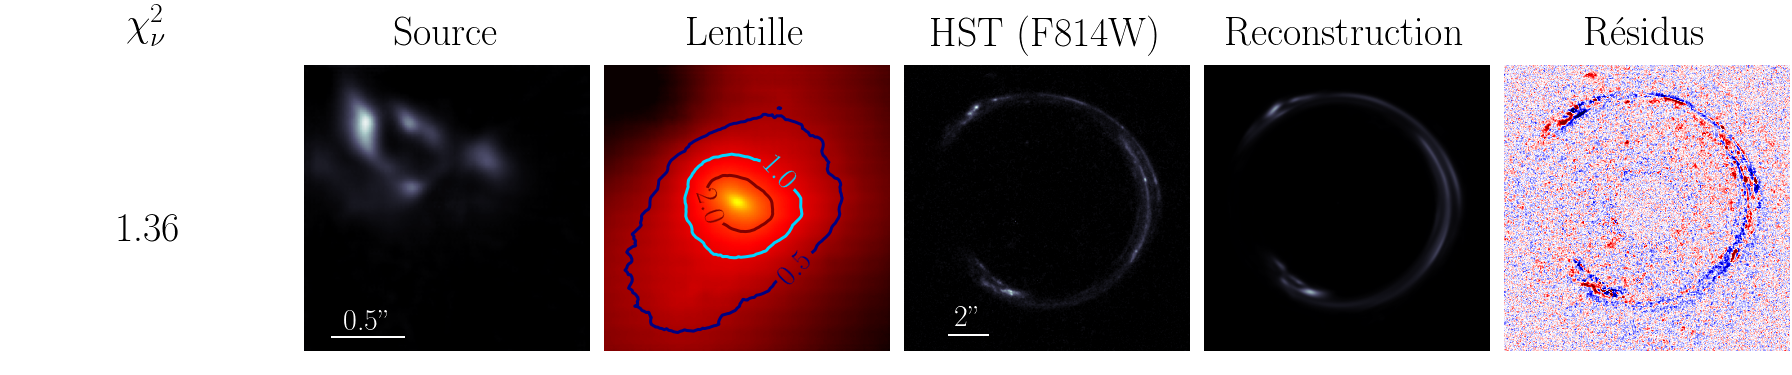
\includegraphics[width=\textwidth]{figures/horseshoe_pred2}
        \caption{Reconstruction du fer à cheval cosmique avec la machine à inférence récurentielle 
        décrite dans le chapitre \ref{chap:censai}.}
        \label{fig:horseshoe}
\end{figure}


        %\selectlanguage{english}
  {\scriptsize
    \bibliography{intro_bib,censai_bib}
  }
  \appendix
  \chapter{$\Lambda$CDM}\label{app:lcdm}

% Décrire la densité critique et d'ou vien Omega here.

\begin{table}[H]
        \centering
        \caption{Paramètres de $\Lambda$CDM ajusté avec les observations du fond diffus cosmologique par le téléscope Planck \citep{PlanckCollaboration2018}}
        \label{tab:cosmos}
        \begin{tabular}{ccc}
                \hline
                Paramètre & Description & Valeur \\\hline \hline
                $\Omega_{r,0}$ & Densité de la radiation & $\sim 10^{-4}$\\
                $\Omega_{m,0}$  &Densité de la matière & 0.3158 \\
                $\Omega_{c,0}h^{2}$  & Densité de la matière noire & 0.12011\\
                $\Omega_{b,0}h^{2}$ & Densité de la matière baryonique & 0.022383\\
                $\Omega_{\Lambda,0}$ &Densité de l'énergie sombre & 0.6842\\
                $\Omega_0$ & Densité totale & $\equiv 1$\\
                $h$ & Constante de Hubble $h \equiv \dfrac{H_0}{100\, \mathrm{km}\,\mathrm{s}^{-1}\, \mathrm{Mpc^{-1}}}$ & $0.6732$ \\
               \hline 
        \end{tabular}
\end{table}


  \selectlanguage{english}
  \chapter{Elastic Weight Consolidation}\label{ap:ewc}

Suppose we are given a training set $\mathcal{D}$ and a test task $\mathcal{T}$. The 
posterior of the RIM parameters $\mathcal{\varphi}$ can be rewritten using the Bayes rule as
\begin{equation}
        p(\varphi \mid \mathcal{D},\, \mathcal{T}) = 
        \frac{p(\mathcal{T} \mid \mathcal{D},\, \varphi) p(\varphi \mid \mathcal{D})}
        {p(\mathcal{T} \mid \mathcal{D})}.
\end{equation} 
We suppose that $\varphi$ encode 
information about $\mathcal{D}$, while $\mathcal{T}$ was unseen by $\varphi$. 
It follows that 
$\mathcal{T}$ and $\mathcal{D}$ are conditionally independent when given $\varphi$. 
We do not make the stronger assumption that $\mathcal{D}$ and $\mathcal{T}$ 
are completely independent. In fact, such an assumption 
would contradict the premiss of our work that building a 
dataset $\mathcal{D}$ can inform a machine (RIM) about
task $\mathcal{T}$ --- or that, more broadly, $\mathcal{D}$ 
contains information about $\mathcal{T}$.

We rewrite the marginal $p(\mathcal{T} \mid \mathcal{D})$ using the Bayes rule
in order to extract $p(\mathcal{D} \mid \mathcal{T})$, 
the sampling distribution used to compute the Fisher diagonal elements
\begin{equation}
        p(\varphi \mid \mathcal{D},\, \mathcal{T}) = 
\frac{p(\mathcal{T} \mid \varphi) p(\varphi \mid \mathcal{D})}
        {p(\mathcal{D} \mid \mathcal{T})}
        \frac{p(\mathcal{D})}{p(\mathcal{T})}.
\end{equation} 
The log-likelihood $\log p(\mathcal{T} \mid \varphi)$ is equivalent to 
the negative of the loss function for the particular task at hand.
In this work, we assign a uniform probability density to $p(\mathcal{T})$ and $p(\mathcal{D})$ 
in order to ignore them.

We now turn to the prior $p(\varphi \mid \mathcal{D})$, which 
appears as a conditional relative to 
the training dataset. 
We use the Laplace approximation around the maxima $\varphi^{\star}_{\mathcal{D}}$ 
to evaluate the prior,
where $\varphi^{\star}_{\mathcal{D}}$ 
are the trained parameters of the RIM that minimize the empirical risk (equation \eqref{eq:Cost}). 
The Taylor expansion of the prior around this maxima yields
\begin{equation}\label{app:prior}
        \log p(\varphi \mid \mathcal{D}) \approx \log p(\varphi^{\star}_{\mathcal{D}} \mid \mathcal{D}) 
        + \frac{1}{2} (\varphi - \varphi^{\star}_{\mathcal{D}})^{T} 
        \underbrace{
        \bigg(
                \frac{\partial^2 \log p(\varphi \mid \mathcal{D})}{\partial^2 \varphi}\bigg|_{\varphi^{\star}_{\mathcal{D}}}
        \bigg)
}_{\displaystyle \mathbf{H}(\varphi^{\star}_{\mathcal{D}})}
        (\varphi - \varphi^{\star}_{\mathcal{D}}).
\end{equation} 
Since $\varphi^{\star}_{\mathcal{D}}$ is an extrema of the prior, the linear term vanishes. 
The empirical estimate of the negative hessian matrix is the observed Fisher information 
matrix which can be written as
\begin{equation}\label{app:fisher}
        \mathcal{I}(\varphi^{\star}_{\mathcal{D}}) = 
        -\EX_{\mathcal{D} \mid \mathcal{T}} [\mathbf{H}(\varphi^{\star}_{\mathcal{D}})] = 
        \EX_{\mathcal{D}\mid \mathcal{T}}
        \Bigg[
                \Bigg(
                \bigg( 
                        \frac{\partial \log p(\varphi \mid \mathcal{D})}{\partial \varphi}
                \bigg) 
                \bigg( 
                        \frac{\partial \log p(\varphi \mid \mathcal{D})}{\partial \varphi}
                \bigg)^{T}
        \Bigg)
\Bigg|_{\varphi^{\star}_{\mathcal{D}}}\Bigg].
\end{equation} 
The expectation is taken over the sample space $p(\mathcal{D} \mid \mathcal{T})$ since 
the network parameters are held fixed during sampling.
In order to compute the Fisher score, 
we apply the Bayes rule to the prior to extract a loss function,
% \begin{equation} 
%         \log p(\varphi \mid \mathcal{D}) = \log p(\mathcal{D}\mid \varphi) 
%         + \log p(\varphi) - \log p(\mathcal{D}).
% \end{equation} 
% $p(\mathcal{D} \mid \varphi)$ is the negative of a loss function, 
which we take to be 
proportional to the training loss (equation \eqref{eq:Loss}) and the $\chi^2$:
\begin{equation}\label{eq:LossFisher}
        \log p\big(\varphi \mid (\mathbf{x}, \mathbf{y}) = \mathcal{D}\big) \propto -\mathcal{L}_{\varphi}(\mathbf{x}, \mathbf{y}) + \frac{1}{T}\sum_{t=1}^{T}\log p(\mathbf{y} \mid \mathbf{\hat{x}}^{(t)}) - \frac{\ell_2}{2}\lVert \varphi \rVert^2_2
\end{equation} 
% The derivative of $\log p(\varphi)$ remains constant when taking 
% the expectation in \eqref{app:fisher}.
We find in practice the the $\ell_2$ term has little effect on the 
Fisher diagonal and our results. Thus, we set $\ell_2 = 0$.

Since the full Fisher matrix is intractable for a neural network, we approximate the 
quadratic term of the prior with the diagonal of the Fisher matrix following \citet{Kirkpatrick2016}. 
For an optimisation problem, the first term of \eqref{app:prior} is constant. Thus,
the posterior becomes proportional to
\begin{equation}
        \log p(\varphi \mid \mathcal{D}, \mathcal{T}) \propto 
        \log p(\mathcal{T} \mid \varphi ) - 
         \frac{\lambda}{2} 
        \sum_{j}\mathrm{diag}(\mathcal{I}(\varphi^{\star}_{\mathcal{D}}))_{j}(\varphi_j - [\varphi^{\star}_{\mathcal{D}}]_j)^2.
\end{equation} 
The Lagrange multiplier $\lambda$ is introduced to tune our uncertainty about the network parameters 
during fine-tuning.

\chapter{VAE Architecture and optimisation}

For the following architectures, we employ the notion of \textit{level} 
to mean layers in the encoder and the decoder with the same resolution. 
In each level, we place a block of convolutional layers 
before downsampling (encoder) or after upsampling (decoder). These operations 
are done with strided convolutions like in the U-net architecture of the RIM.

\begin{table}[H]
%\begin{minipage}{.5\linewidth} 
        \centering
        \caption{Hyperparameters for the background source VAE.}
        \label{tab:Source VAE}
        \begin{tabular}{cc}
                Parameter & Value \\\hline\hline
                Input preprocessing & $\bbone$ \\
                                    & \\

                \textit{Architecture} & \\
                Levels (encoder and decoder) & 3 \\
                Convolutional layer per level & 2 \\
                Latent space dimension & 32\\
                Hidden Activations & Leaky ReLU \\
                Output Activation & Sigmoid \\
                Filters (first level) & 16 \\
                Filters scaling factor (per level) & 2 \\
                Number of parameters & $3\,567\,361$\\

                           & \\
                \textit{Optimization} & \\
                Optimizer & Adam \\
                Initial learning rate & $10^{-4}$ \\
                Learning rate schedule & Exponential Decay \\
                Decay rate & 0.5 \\
                Decay steps & $30\,000$ \\
                Number of steps & $500\,000$ \\
                $\beta_{\mathrm{max}}$ & 0.1 \\
                Batch size & 20\\
                \hline
        \end{tabular}
\end{table}
%\end{minipage}
%\begin{minipage}{.5\linewidth}
\begin{table}[H]
        \centering
        \caption{Hyperparameters for the convergence VAE.}
        \label{tab:Kappa VAE}
        \begin{tabular}{cc}
                Parameter & Value \\\hline\hline
                Input preprocessing & $\log_{10}$ \\
                              & \\

                \textit{Architecture} & \\
                Levels (encoder and decoder) & 4 \\
                Convolutional layer per level & 1 \\
                Latent space dimension & 16\\
                Hidden Activations & Leaky ReLU \\
                Output Activation & $\bbone$ \\
                Filters (first level) & 16 \\
                Filters scaling factor (per level) & 2 \\
                Number of parameters & $1\,980\,033$\\


                           & \\
                \textit{Optimization} & \\
                Optimizer & Adam\\
                Initial learning rate & $10^{-4}$ \\
                Learning rate schedule & Exponential Decay \\
                Decay rate & 0.7 \\
                Decay steps & $20\,000$ \\
                Number of steps & $155\,000$ \\
                $\beta_{\mathrm{max}}$ & 0.2 \\
                Batch size & 32\\
                \hline
        \end{tabular}
%\end{minipage}
\end{table}

\chapter{RIM architecture and optimisation}\label{ap:rim training and opt}

The notion of link function $\Psi: \Xi \rightarrow \mathcal{X}$, 
introduced by \citet{Putzky2017}, is an invertible transformation 
between the network prediction space $\boldsymbol{\xi} \in \Xi$ 
and the forward modelling space $\mathbf{x} \in \mathcal{X}$.
This is a different notion from preprocessing, discussed in section \ref{sec:data}, 
because this transformation is applied inside the recurrent relation \ref{eq:RIM} 
as opposed to before training. In the case where the forward model has some restricted 
support or it is found that some transformation helps the training, then 
the link function chosen must be implemented as part of the network architecture as 
shown in the unrolled computational graph in Figure \ref{fig:unrolled graph}.
Also, the loss $\mathcal{L}_\varphi$ must be computed in the $\Xi$ space in order 
to avoid gradient vanishing problems when $\Psi$ is a non-linear mapping, which 
happens if the non-linear link function is applied in an 
operation recorded for backpropagation through time (BPTT). 
For the convergence, we use an exponential link function with base $10$: 
$\boldsymbol{\hat{\kappa}} = \Psi(\boldsymbol{\xi}) = 10^{\boldsymbol{\xi}}$. 
This $\Psi$ encodes the non-negativity of the convergence. Furthermore, 
it is a power transformation that leaves the linked 
pixel values $\boldsymbol{\xi}_i$ normally distributed, thus improving the 
learning through the non-linearities in the neural network.

The pixel weights $\mathbf{w}_i$ in the loss function \eqref{eq:Loss}
are chosen to encode the fact that the pixel with critical mass density ($\boldsymbol{\kappa}_i > 1$) 
have a stronger effect on the lensing configuration than other pixels. 
We find in practice that the weights 
\begin{equation}\label{eq:convergence weights} 
        \mathbf{w}_i = \frac{\sqrt{\boldsymbol{\kappa}_i}}{ \sum_i \boldsymbol{\kappa}_i}, 
\end{equation} 
encode this knowledge in the loss function and improved both the empirical 
risk and the goodness of fit of the baseline model on early test runs.

For the source, we found that we do not need a link function 
--- the identity is generally better compared to other link function we tried like sigmoid and 
power transforms --- and we found that the pixel weights can be taken to 
be uniform, i.e. $\mathbf{w}_i = \frac{1}{M}$.


\begin{figure}[H]
        \centering
        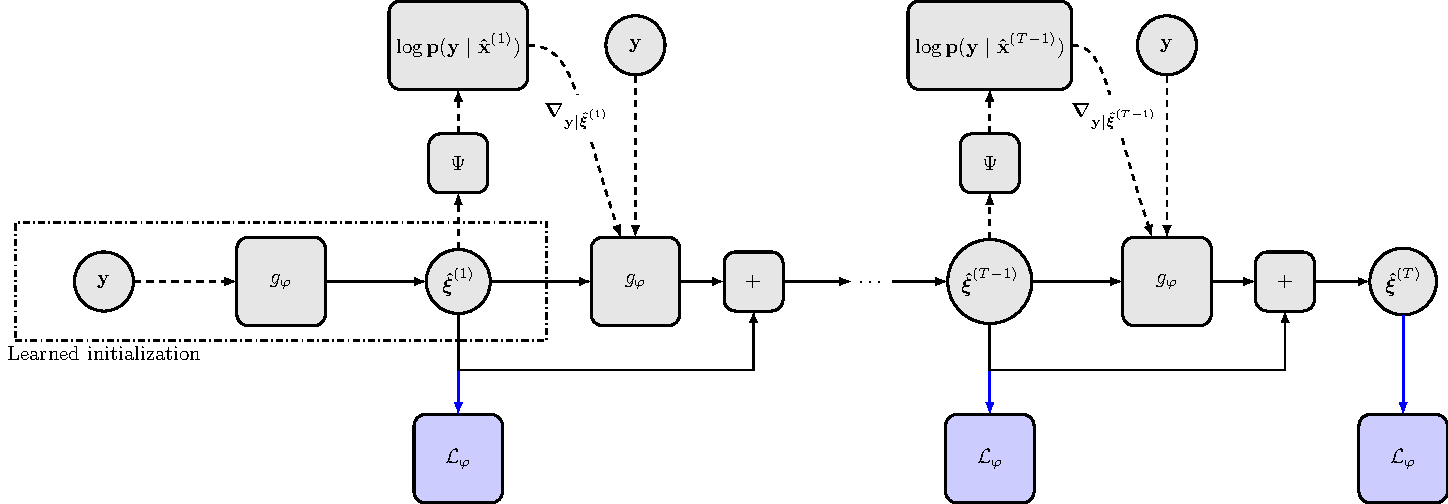
\includegraphics[width=\linewidth]{figures/schematic_rim_unrolled}
        \caption{Unrolled computational graph of the RIM. Operations along solid arrows are being 
        recorded for BPTT, while operations along dashed arrows are not. The blue arrows are only 
        used for optimisation during training. During fine-tuning or testing, the loss is computed only 
        as an oracle metric to validate that our methods can recover the ground truth.}
        \label{fig:unrolled graph}
\end{figure}
\begin{table}[H]
        \centering
        \caption{Hyperparameters for the RIM.}
        \label{tab:baseline hparams}
        \begin{tabular}{cc}
                Parameter & Value \\\hline\hline
                Source link function & $\bbone$ \\
                $\kappa$ link function & $10^{\boldsymbol{\xi}}$ \\
                                       & \\
                \textit{Architecture} & Figure \ref{fig:unet} \\
                Recurrent steps ($T$) & 8 \\
                Number of parameters & $348\,546\,818$ \\
                                      & \\
                \textit{First Stage Optimisation} & \\
                Optimizer & Adamax \\
                Initial learning rate & $10^{-4}$\\
                Learning rate schedule & Exponential Decay \\
                Decay rate & 0.95 \\
                Decay steps & $100\,000$\\
                Number of steps & $610\,000$\\
                Batch size & 1 \\
                           & \\
                \textit{Second Stage Optimisation} & \\
                Optimizer & Adamax \\
                Initial learning rate & $6\times 10^{-5}$\\
                Learning rate schedule & Exponential Decay \\
                Decay rate & 0.9 \\
                Decay steps & $100\,000$\\
                Number of steps & $870\,000$\\
                Batch size & 1 \\
                
                \hline
        \end{tabular}
\end{table}


%\begin{figure}[H]
        %\centering
        %\begin{tikzpicture}
                %\tikzstyle{every node}=[font=\scriptsize]
                %\node at (0, 0) {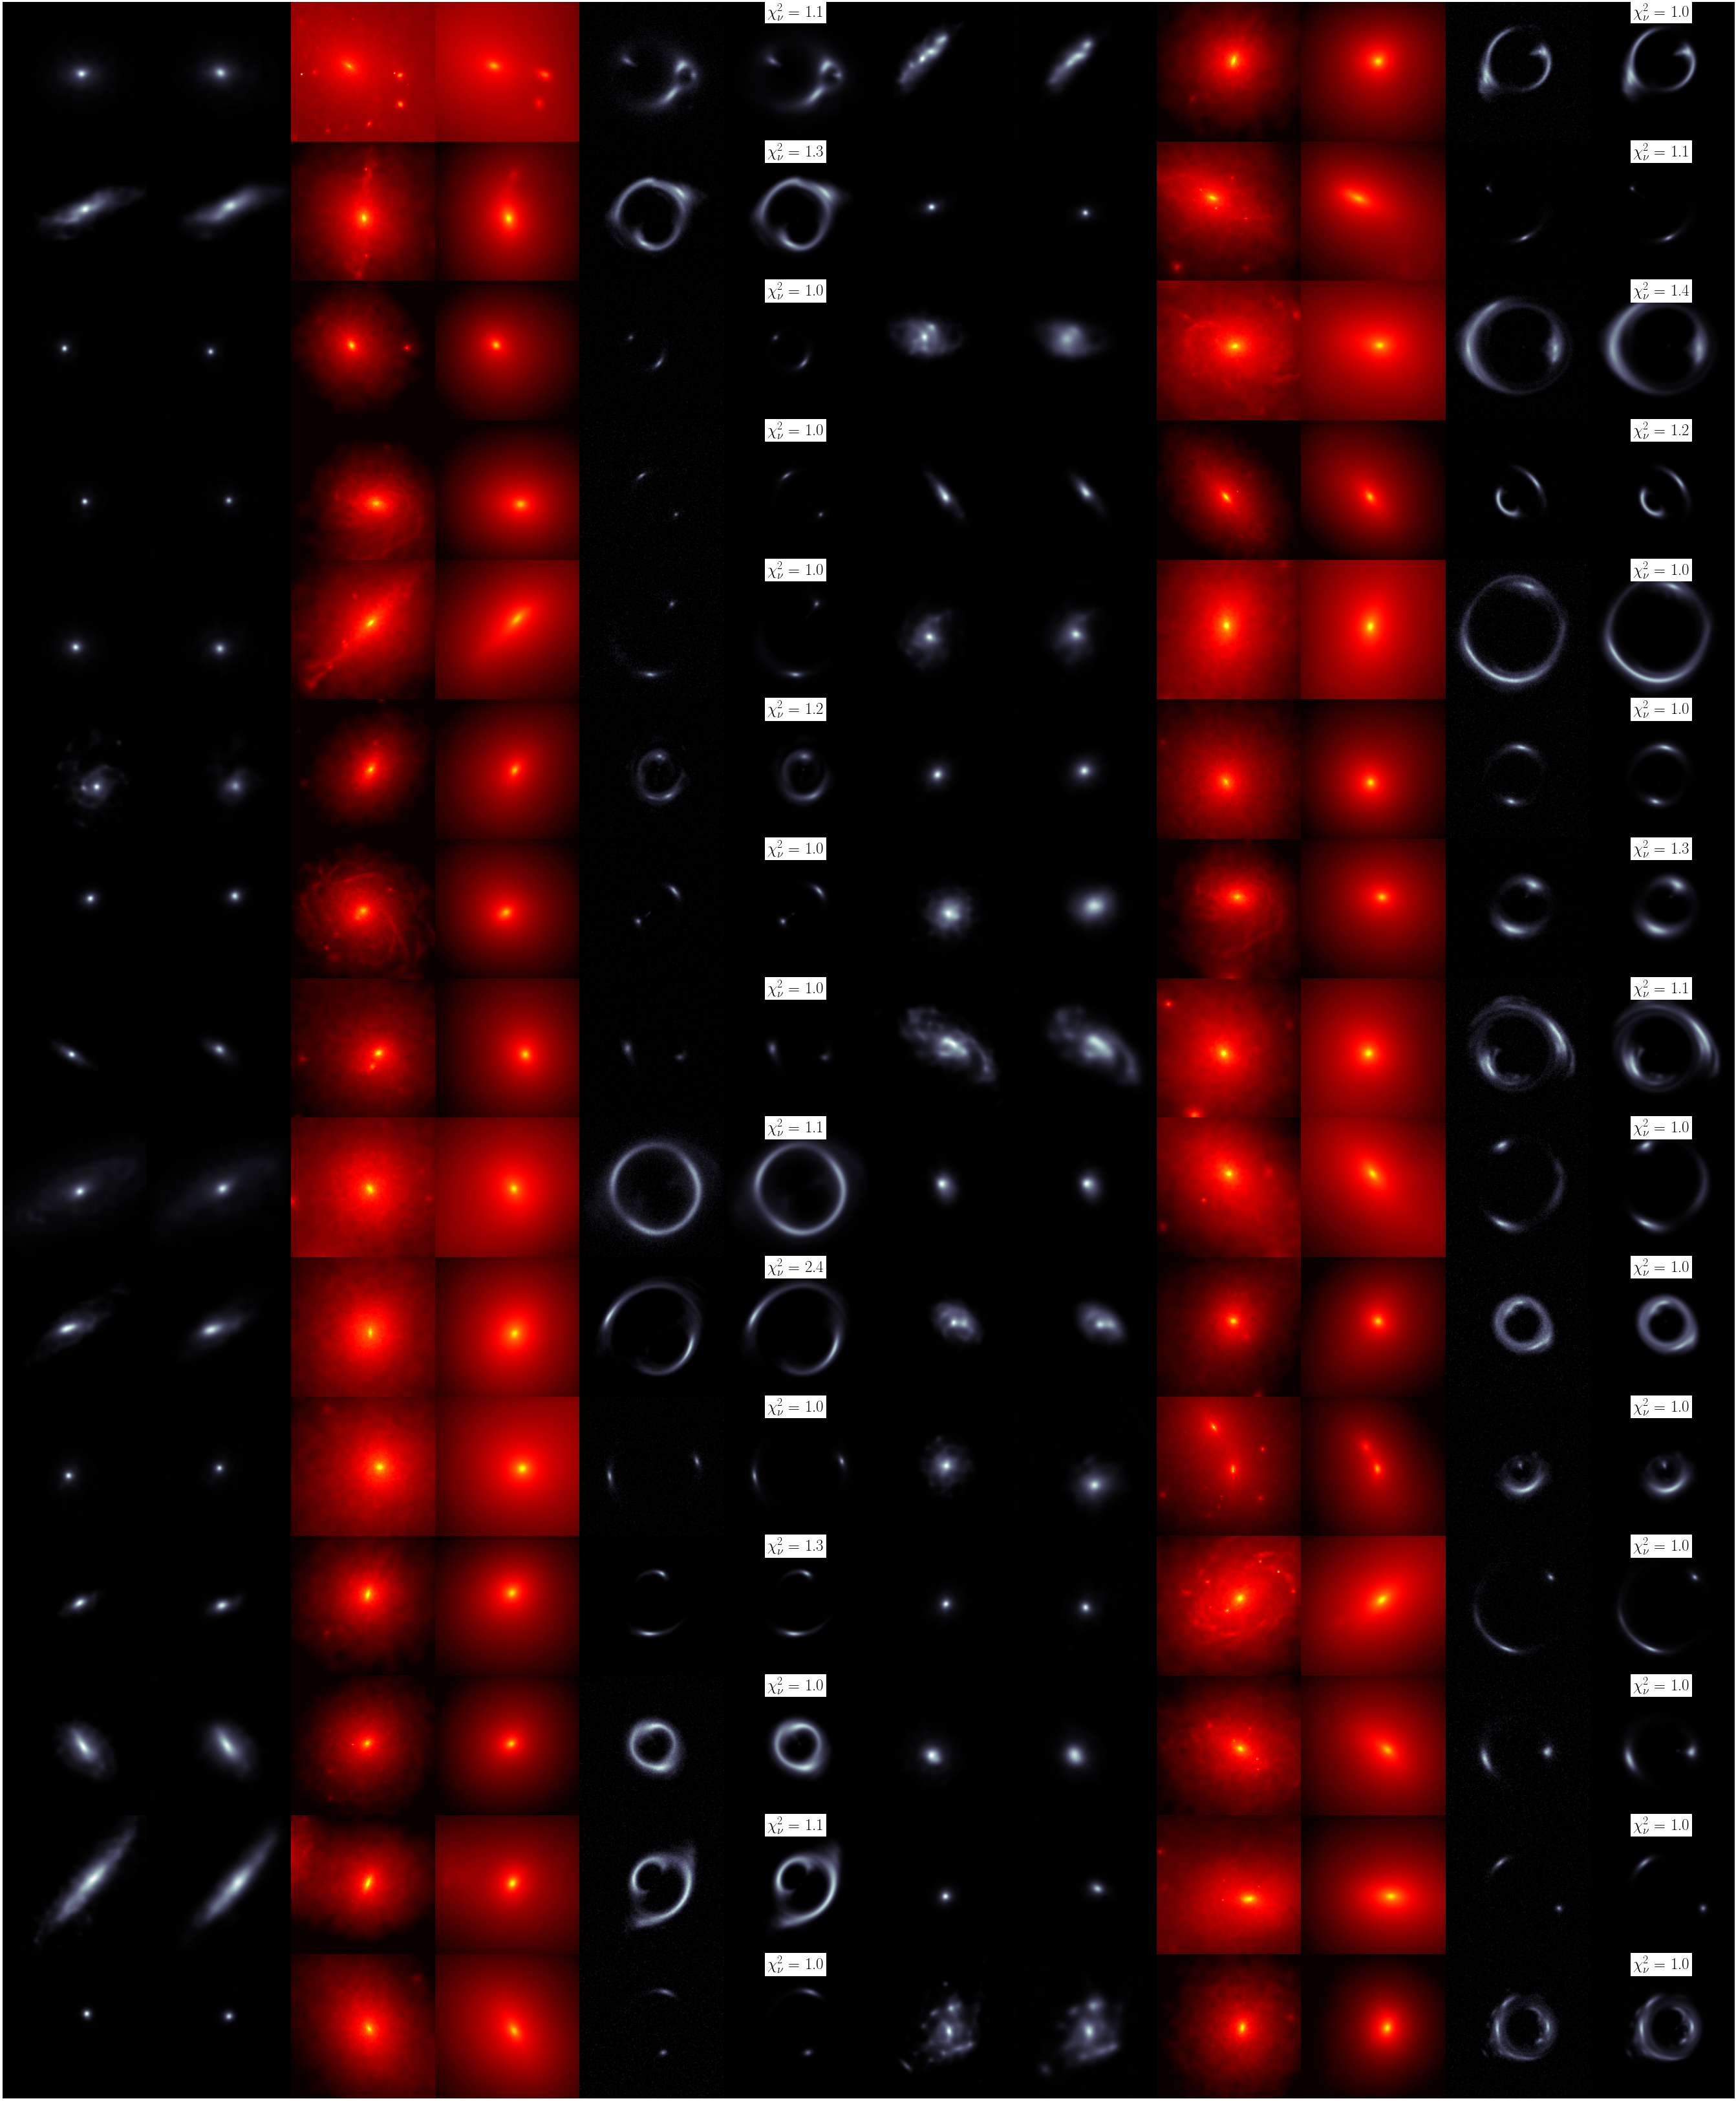
\includegraphics[width=\linewidth]{figures/test_set_no_cherry_pick}};
                %\node at (-8.2, 11) {COSMOS\strut};
                %\node at (-6.8, 11) {RIM+FT\strut};
                %\node at (-5.3, 11) {IllustrisTNG\strut};
                %\node at (-3.7, 11) {RIM+FT\strut};
                %\node at (-2.2, 11) {Observation\strut};
                %\node at (-0.8, 11) {RIM+FT\strut};

                %\node at (0.6, 11) {COSMOS\strut};
                %\node at (2.1, 11) {RIM+FT\strut};
                %\node at (3.7, 11) {IllustrisTNG\strut};
                %\node at (5.2, 11) {RIM+FT\strut};
                %\node at (6.7, 11) {Observation\strut};
                %\node at (8.2, 11) {RIM+FT\strut};

                
                %% \node at (-7.5, 11.2) {COSMOS};
                %% \node at (-4.5, 11.2) {RIM+FT};
                %% \node at (-6, 11.7) {Sources};
                %% \node at (-1.5, 11.2) {Illustris TNG};
                %% \node at (1.5, 11.2) {RIM+FT};
                %% \node at (0, 11.7) {Convergence};
                %% \node at (4.5, 11.2) {Observation};
                %% \node at (7.5, 11.2) {RIM+FT};
        %\end{tikzpicture}
        %\caption{
                %30 reconstructions taken at random from the test set of 3000 examples simulated from COSMOS 
                %and IllustrisTNG data at high SNR.
                %The colorscale are the same as in Figure \ref{fig:main result}.}
        %\label{fig:random sample}
%\end{figure}


\selectlanguage{french}
  \chapter{GRU}\label{ap:gru}
Une unité récurrente à porte convolutionnelles est décrite par les opérations
\begin{align}
		\tilde{\mathbf{x}} &= S\bigg( \mathbf{w}_o * (\mathbf{h}^{(t-1)} \oplus \mathbf{x}^{(t)}) + \mathbf{b}_o\bigg) &\{\text{Porte d'oubli}\} \\
		\mathbf{z} &= S\bigg( \mathbf{w}_z * (\mathbf{h}^{(t-1)} \oplus \mathbf{x}^{(t)}) + \mathbf{b}_{z}\bigg)&\{\text{Porte de mise à jour}\} \\
		\tilde{\mathbf{h}} &= \tanh\bigg( \mathbf{w}_h * \big((\mathbf{h}^{(t-1)}\odot \tilde{\mathbf{x}}) \oplus \mathbf{x}^{(t)})\big) + \mathbf{b}_{h}\bigg)&\{\text{État candidat}\} \\
	\label{eq:nouvel etat}
		\mathbf{h}^{(t)} &=\mathbf{h}^{(t-1)} \odot \mathbf{z} + \tilde{\mathbf{h}} \odot (1 - \mathbf{z}) &\{\text{Nouvel état}\} 
\end{align}
où $S(x) = \frac{1}{1 + e^{-x}}$ est une fonction sigmoïde et $\mathbf{x}^{(t)}$ est un tenseur à l'entrée de l'unité. 
Les noyaux de convolution $\mathbf{w}$ et les vecteurs de biais $\mathbf{b}$  
sont des paramètres libres appris par descente de gradient stochastique. $\oplus$ symbolise l'opération 
de concatenation. Le tenseur de sortie de cette unité, soit le nouvel état latent $\mathbf{h}^{(t)}$, 
est une combinaison de l'état latent précédent $\mathbf{h}^{(t-1)}$ et de l'état candidat 
$\tilde{\mathbf{h}}$, pesée élément par élément par le vecteur à la sortie de la porte de mise à jour $\mathbf{z}$.


  \chapter{Congrès où l'étudiant à présenté ses résultats}

\section*{IVADO Digital October}
\textbf{Médium}: Présentateur \\
\textbf{Titre}: Pixelated Reconstruction of Gravitational Lenses using Recurrent Inference Machine \\
\textbf{Lieu}: En ligne\\
\textbf{Année}: 2021\\
\textbf{Auteurs}: A. Adam, L Perreault-Levasseur et Y. Hezaveh


\section*{Likelihood-free in Paris}
\textbf{Médium}: Affiche\\
\textbf{Titre}: Pixelated Reconstruction of Gravitational Lenses using Recurrent Inference Machine \\
\textbf{Lieu}: Paris, France\\
\textbf{Année}: 2022\\
\textbf{Auteurs}: A. Adam, L Perreault-Levasseur et Y. Hezaveh

\section*{CRAQ Annual Meeting}
\textbf{Médium}: Présentateur\\
\textbf{Titre}: Pixelated Reconstruction of Gravitational Lenses using Recurrent Inference Machine \\
\textbf{Lieu}: Orford, Qc\\
\textbf{Année}: 2022\\
\textbf{Auteurs}: A. Adam, L Perreault-Levasseur et Y. Hezaveh

\section*{CASCA Annual Meeting}
\textbf{Médium}: Affiche\\
\textbf{Titre}: Pixelated Reconstruction of Gravitational Lenses using Recurrent Inference Machine \\
\textbf{Lieu}: En ligne\\
\textbf{Année}: 2022\\
\textbf{Auteurs}: A. Adam, L Perreault-Levasseur et Y. Hezaveh

\section*{Machine Learning for Astrophysics
Workshop at the Thirty-ninth International Conference on Machine Learning (ICML 2022)}
\textbf{Médium}: Affiche\\
\textbf{Titre}: Pixelated Reconstruction of Gravitational Lenses using Recurrent Inference Machine \\
\textbf{Lieu}: Baltimore, MD\\
\textbf{Année}: 2022\\
\textbf{Auteurs}: A. Adam, L Perreault-Levasseur et Y. Hezaveh

\section*{IAIFI Summer School \& Workshop}
\textbf{Médium}: Affiche\\
\textbf{Titre}: Pixelated Reconstruction of Gravitational Lenses using Recurrent Inference Machine \\
\textbf{Lieu}: Boston, MA\\
\textbf{Année}: 2022\\
\textbf{Auteurs}: A. Adam, L Perreault-Levasseur et Y. Hezaveh



\end{document}

